\chapter{Results}
The FD solver and the embedding of the FV solver into FINN were done from scratch. Therefore, in the following part, results will be presented step by step, which will build on each other. Through this approach, we tried to minimize methodological and technical errors to point out deviations and anomalies.
\section{Validation}
Solutions of the FD solver were checked for plausibility using various input conditions and were compared with Hydrus solutions to evaluate its correctness.
\subsection{Plausibility Check}
Based on an initial point concentration at $x=28 cm$ advection processes without dispersion and any sorption processes were simulated. It is plausible that at a set effective velocity of $78.9 \frac{cm}{d}$ the first PFOS reaches the outflow after about $t = 0.3d$ and the mass or concentration of PFOS remains approximately constant over the time before it flows out (Fig. \ref{fig:sol_basic_adv}).
\begin{figure}[h!]
	\centering
	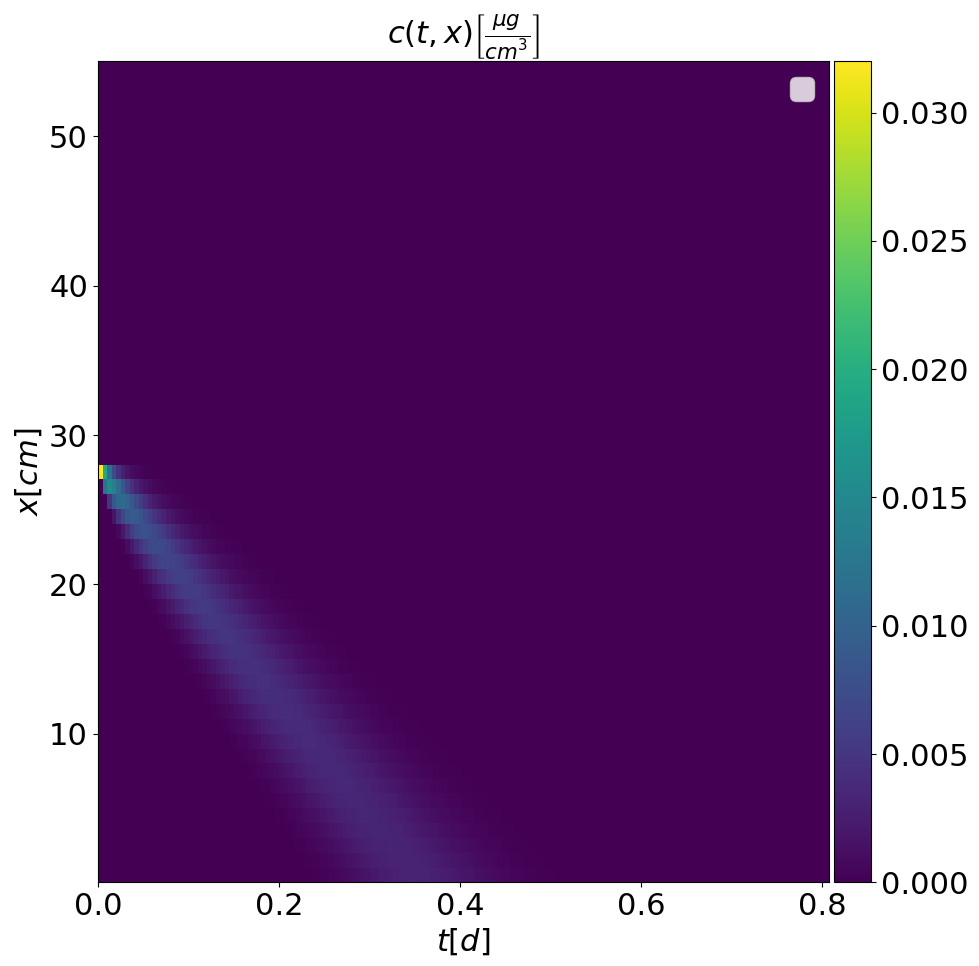
\includegraphics[scale=0.55]{images/sol_basic_adv.png}
\caption[Plausibility check: Advection]{Advection process of initial point concentration without sorption processes.}
\label{fig:sol_basic_adv}
\end{figure}
Without effective velocity but with sorption and diffusion terms respectively, the funnel-shaped concentration spreading of $c$ and $s_k$ can be expected (Fig. \ref{fig:sol_basic_disp}). The kinetically sorbed concentration increases at the beginning, so with eq. \ref{eq:rate_process} we have $(1-f)k_dc^{\beta} > s_k$, which is plausible too.
\begin{figure}[h!]
	\centering
	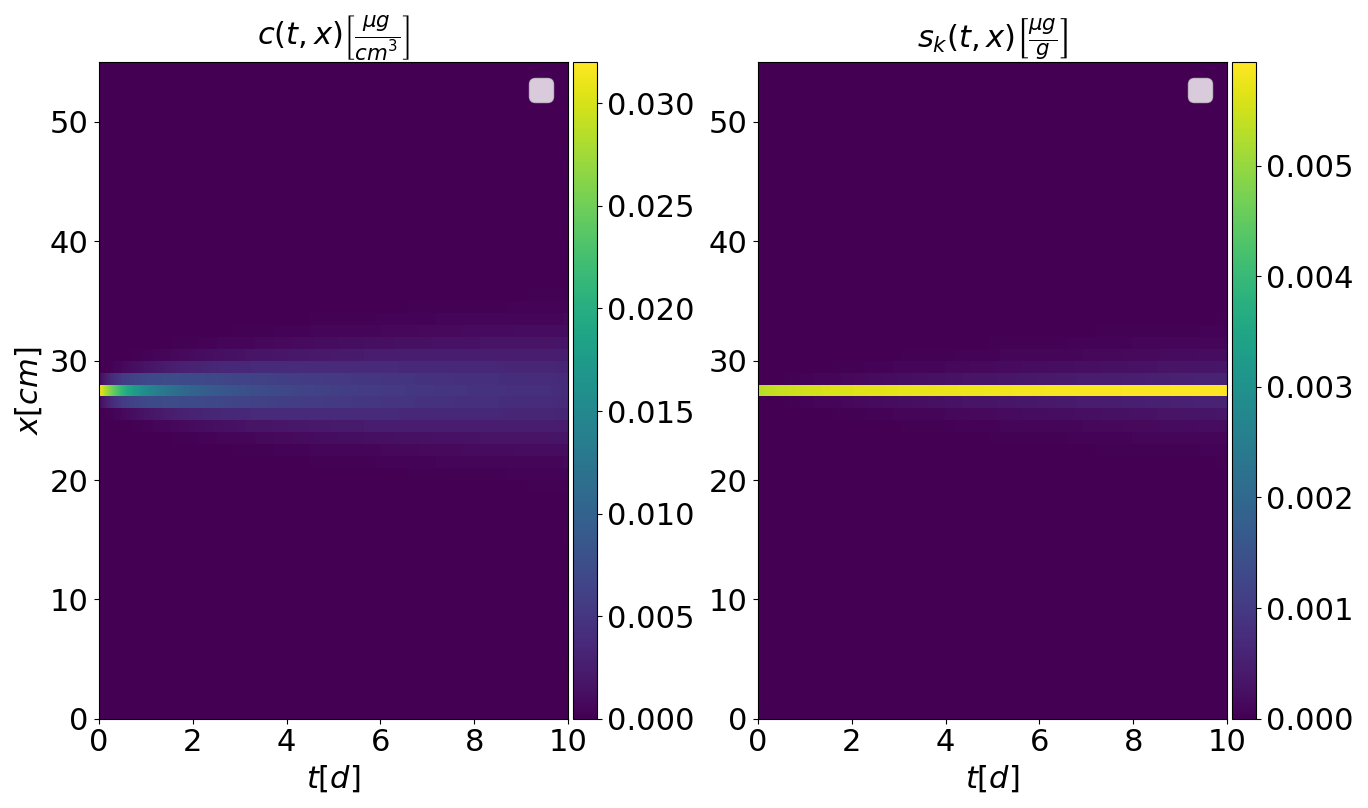
\includegraphics[scale=0.4]{images/sol_basic_disp.png}
\caption[Plausibility check: Dispersion and Sorption]{Diffusion process of initial point concentration with sorption processes.}
\label{fig:sol_basic_disp}
\end{figure}
\FloatBarrier
\subsection{Validation with Hydrus}
A solution of the FD solver (Fig. \ref{fig:sol_ov_hyd_fd}, top left, bottom left) with corresponding parameters (Material parameters: Table \ref{tab:mat_hyd}, Model parameters: Table \ref{tab:mod_hyd}, Discretization parameters: Table \ref{tab:disc_hyd}) was used for validation with Hydrus.
\begin{table}[h!]
    \centering
    \begin{tabular}{ccccccc}
         $n_{e} \left[-\right]$ & $\rho \left[\frac{g}{cm^3}\right]$ & $D_e \left[\frac{cm^2}{d}\right]$ & $\alpha_l \left[cm\right]$ & $c_{init} \left[\frac{\mu g}{cm^3}\right]$ & $s_{k, init} \left[\frac{\mu g}{g}\right]$ & $q \left[\frac{cm}{d}\right]$  \\ [0.2 cm] \hline
         0.4 & 1.58 & 2.5 & 10 & 0.032 & 0.0053 & 20 \\
    \end{tabular}
    \caption{Material parameters used for validation of the solution with Hydrus.}
    \label{tab:mat_hyd}
\end{table}
\begin{table}[h!]
    \centering
\begin{tabular}{ccccc}
     $k_d \left[\frac{cm^3}{d}\right]$ & $\beta \left[-\right]$ & $f \left[-\right]$ & $\alpha_k \left[\frac{1}{d}\right]$ \\ [0.2 cm] \hline
     4.5 & 0.98 & 0.5 & 0.005
\end{tabular}
    \caption{Model parameters used for validation of the solution with Hydrus.}
    \label{tab:mod_hyd}
\end{table}
\begin{table}[h!]
    \centering
    \begin{tabular}{cccccc}
      $T_{MAX} \left[d\right]$ & $T_{STEPS} \left[-\right]$ & $X_{LENGTH} \left[cm\right]$ & $X_{STEPS} \left[-\right]$ \\ [0.2 cm] \hline
      200 & 200000 & 40 & 80
\end{tabular}
    \caption{Discretization parameters used for validation of the solution with Hydrus.}
    \label{tab:disc_hyd}
\end{table}\\
The kinetic sorption process has not yet reached its equilibrium, the large changes in $c$ affect the kinetic sorption behavior. As expected in the solution of the rate process eq. \ref{eq:sol_rate_process}, for large $t$ an exponential decrease was observable (Fig. \ref{fig:hyd_fd_btc}, right).\\
In order to asses the quality of the FD solver a Hydrus solution (Fig. \ref{fig:sol_ov_hyd_fd}, top right, bottom right) with the same parameters was produced. To receive a Darcy flux of $20\frac{cm}{d}$ a vertical flow with column length $L=40cm$, $k_f = 20\frac{cm}{d}$, $h_b = 100cm$ and $h_c = 140cm$ with constant pressure head as boundary condition was chosen.\\
Hydrus values of $c$ and $s_k$ in the last row at given times ($t=0d, ..., 199d$) resulted in a MSE = $4.31 \times 10^{-9}$ for $c$ and MSE = $4.52 \times 10^{-10}$ for $s_k$, with respect to corresponding points in the FD solution (Fig. \ref{fig:hyd_fd_btc}). The MSE complies with the different orders of magnitude of $c$ and $s_k$.
\begin{figure}[h!]
	\centering
	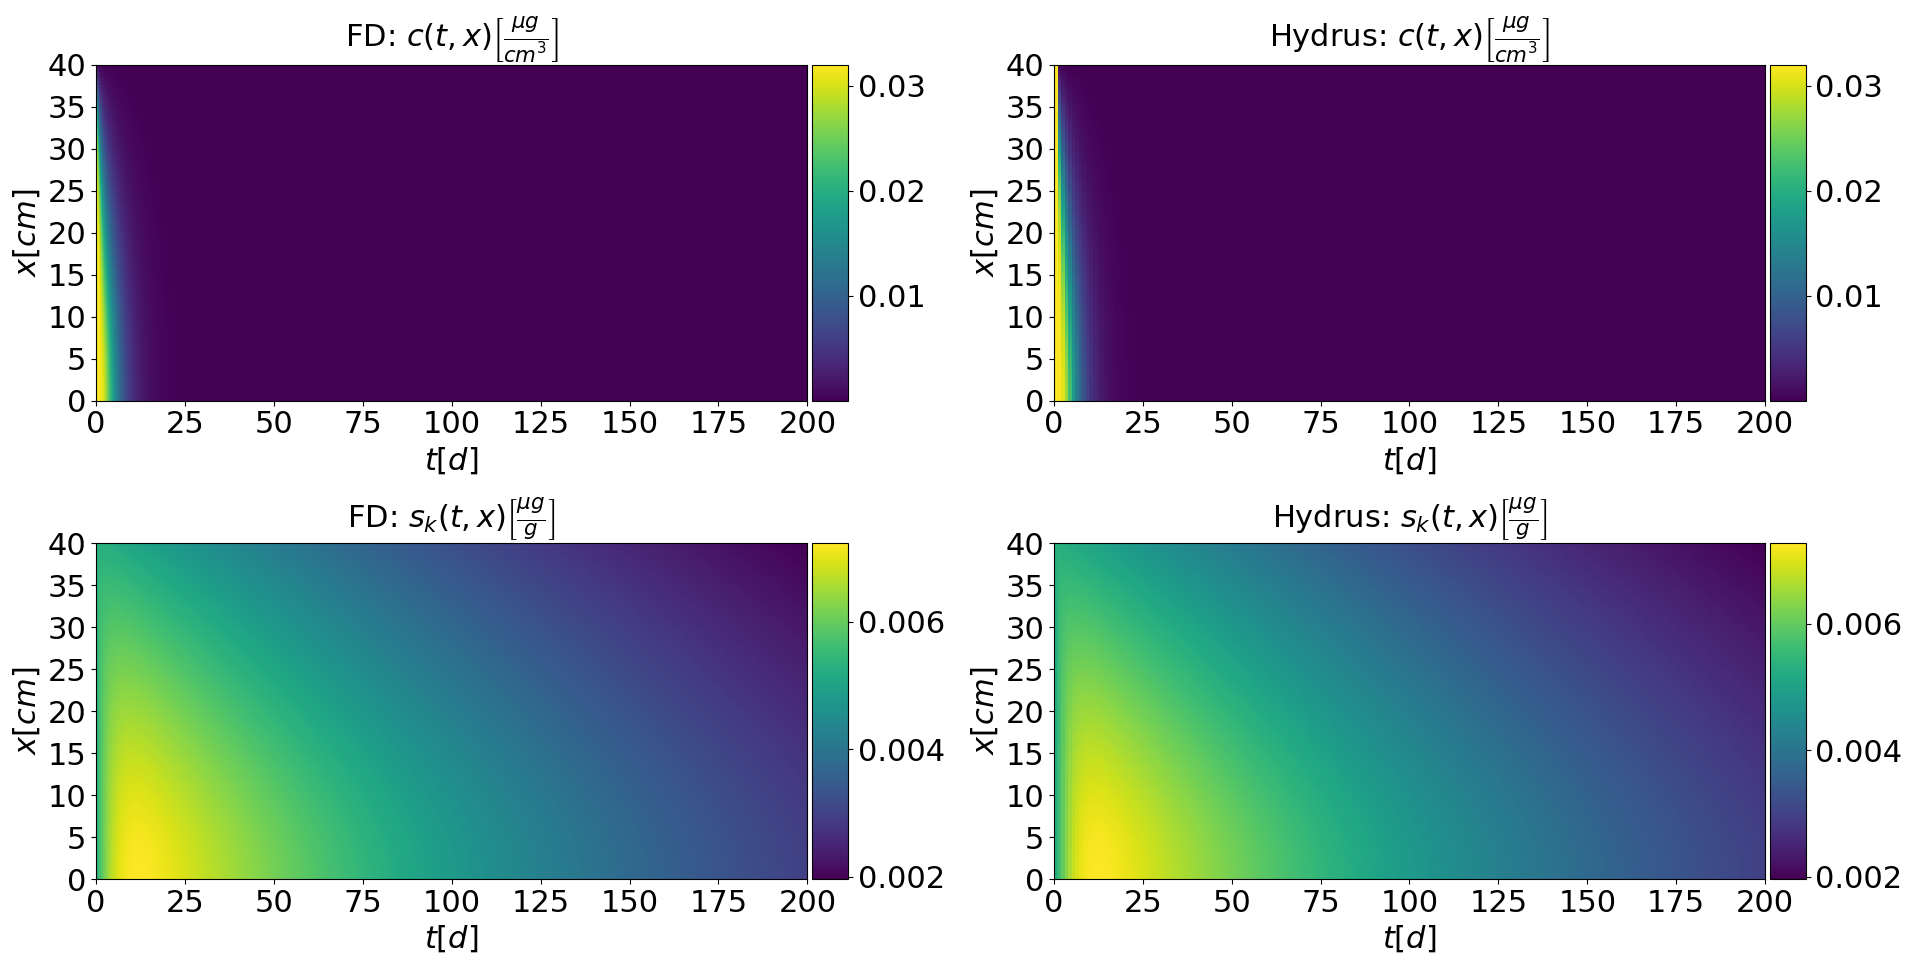
\includegraphics[scale=0.3]{images/sol_ov_hyd_fd.png}
\caption{Comparison of Hydrus and FD solution without sand.}
\label{fig:sol_ov_hyd_fd}
\end{figure}
\begin{figure}[h!]
	\centering
	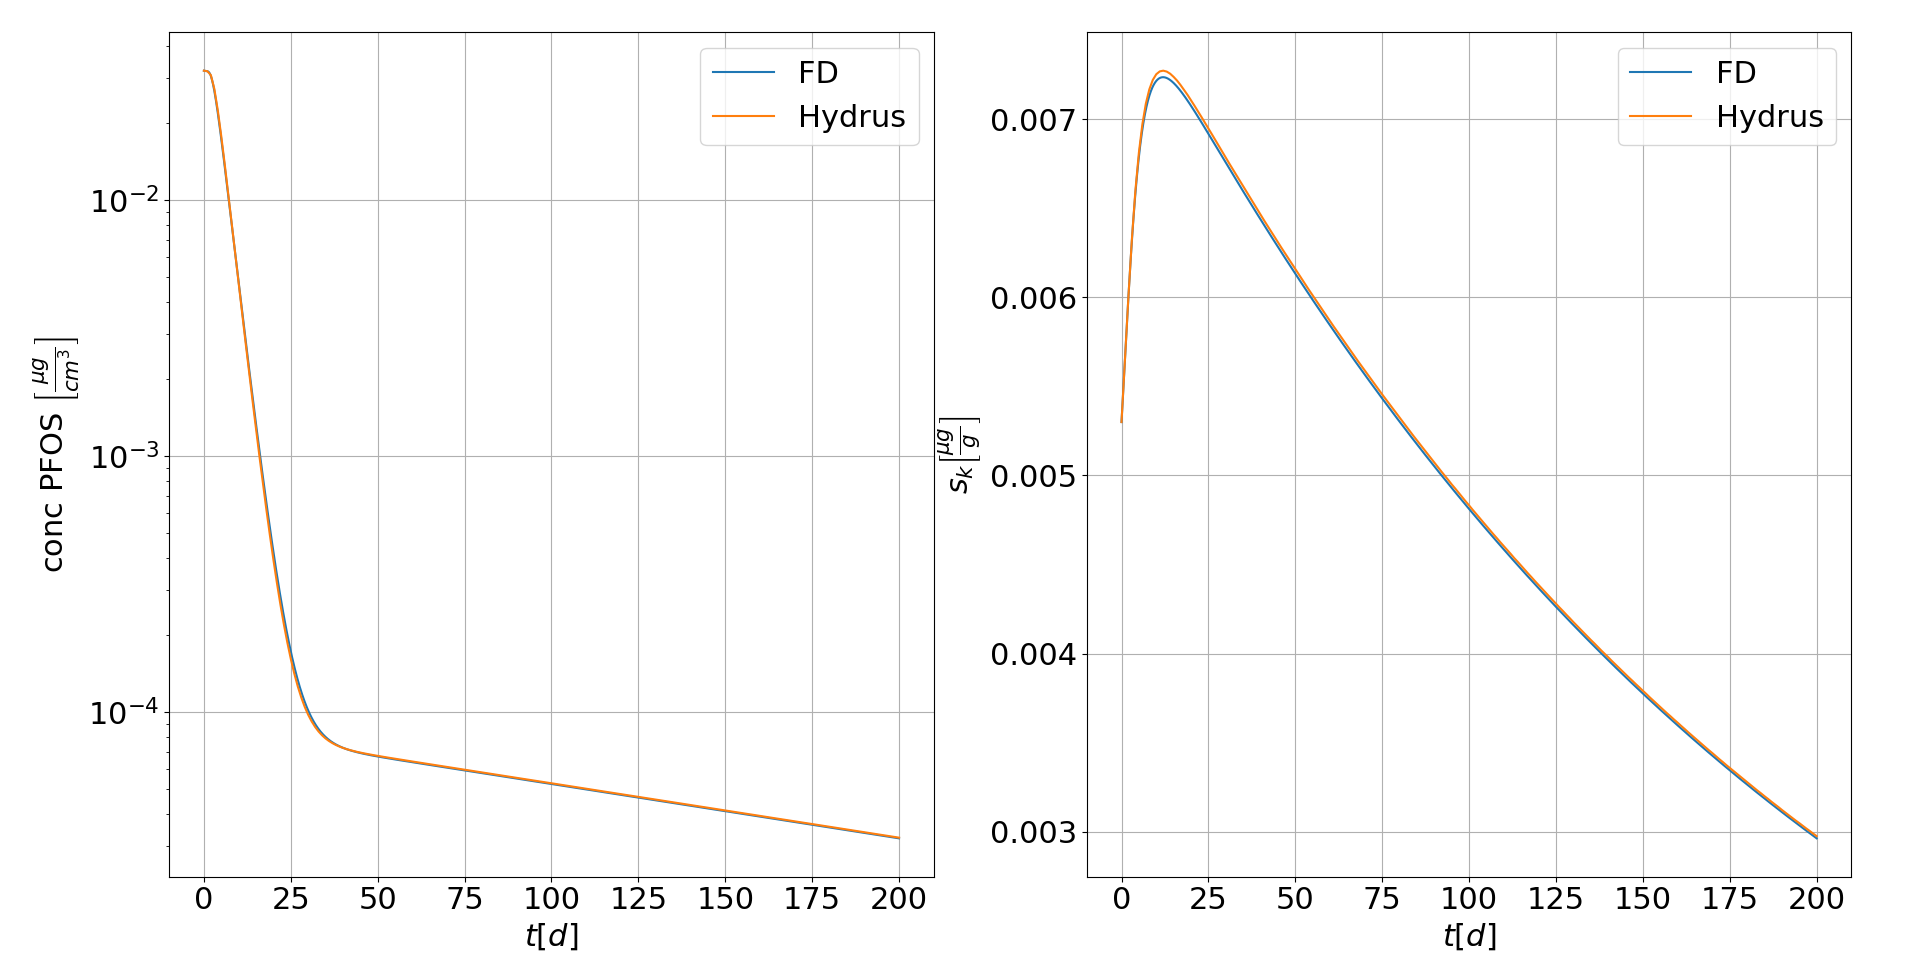
\includegraphics[width=\textwidth]{images/hyd_fd_last_cell.png}
\caption[Comparison of Hydrus and BTC without sand]{Comparison of Hydrus and FD solution without sand: $c$ in bottom row (left), $s_k$ in bottom row (right).}
\label{fig:hyd_fd_btc}
\end{figure}\\
\\
In a next step, the FD solution including sand layers was compared with a corresponding solution generated by Hydrus (Fig. \ref{fig:sol_ov_hyd_fd_sand}). Parameters above were adopted and some were added to describe properties of the sand (Tab. \ref{tab:sand_params}).
\begin{table}[h!]
    \centering
\begin{tabular}{cccc}
     $n_{e, sand} \left[-\right]$&$\alpha_{l, sand} \left[cm\right]$ & top & bot  \\ [0.2 cm] \hline
     0.31 & 5 & 10 & 70 \\
\end{tabular}
    \caption{Sand parameters used for Hydrus validation}
    \label{tab:sand_params}
\end{table}
Using the assumption that no sorption processes occured in the sand layers, sorption parameters or the density of sand were not needed. Molecular diffusion was also neglected in the sand layers.\\
Comparing the BTCs and $s_k$ of the bottom non-sand cell ($x_{bot}$) of the two solutions resulted in larger deviations: $c$: MSE = $1.90 \times 10^{-5}$, $s_k$: MSE = $2.71 \times 10^{-6}$.\\
At times close to $t=0d$ PFOS has not yet flown out of the column, since it must first be transported through the lower sand layer (Fig. \ref{fig:hyd_fd_last_cell_sand}).\\
\\
Further comparisons with other parameters can be found in the appendix (Figs. \ref{fig:hyd_app_1}, \ref{fig:hyd_app_2}, \ref{fig:hyd_app_4}, \ref{fig:hyd_app_5}, \ref{fig:hyd_pde_exp_0.4}, \ref{fig:hyd_pde_exp_0.93},  \ref{fig:hyd_pde_exp_0.99}). As already mentioned, corresponding Hydrus files are available on GitHub \cite{Hydrus_BA}.
\begin{figure}[h!]
	\centering
	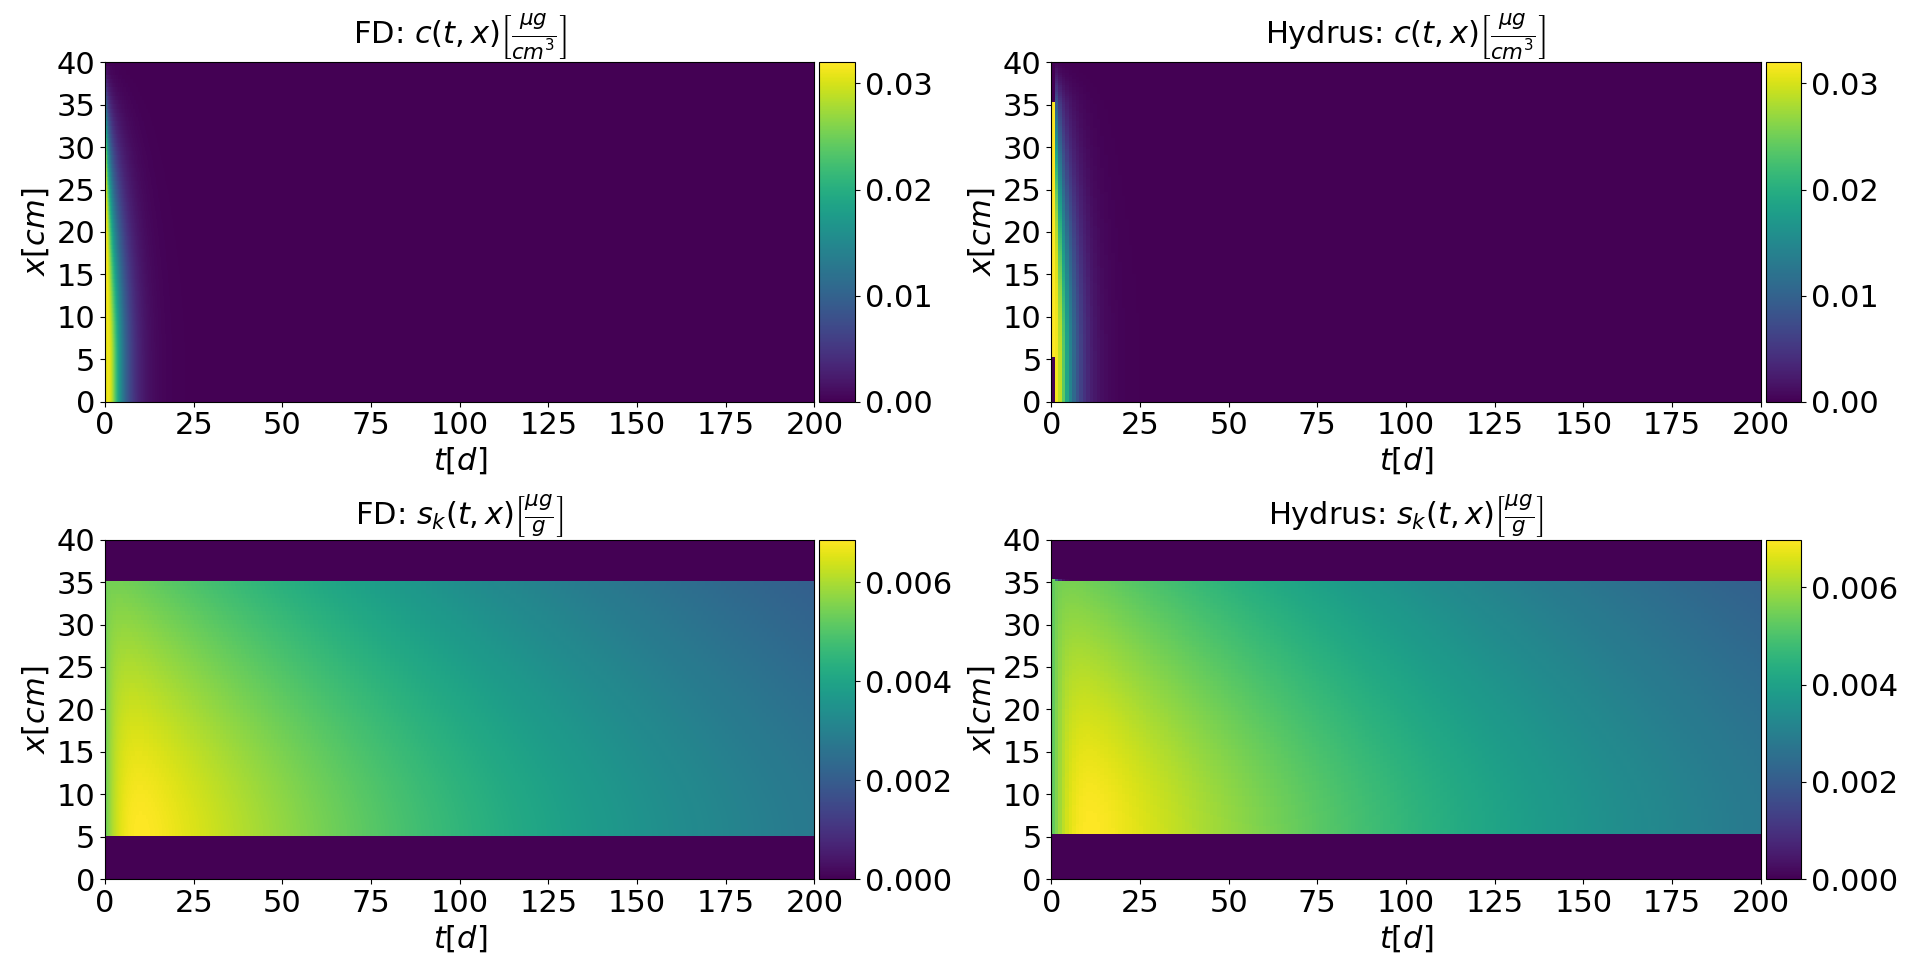
\includegraphics[width=\textwidth]{images/sol_ov_hyd_fd_sand.png}
\caption[Comparison of Hydrus and FD solution with sand]{Comparison of Hydrus and FD solution of $c$ and $s_k$ with 2 sand layers.}
\label{fig:sol_ov_hyd_fd_sand}
\end{figure}
\begin{figure}[h!]
\centering
	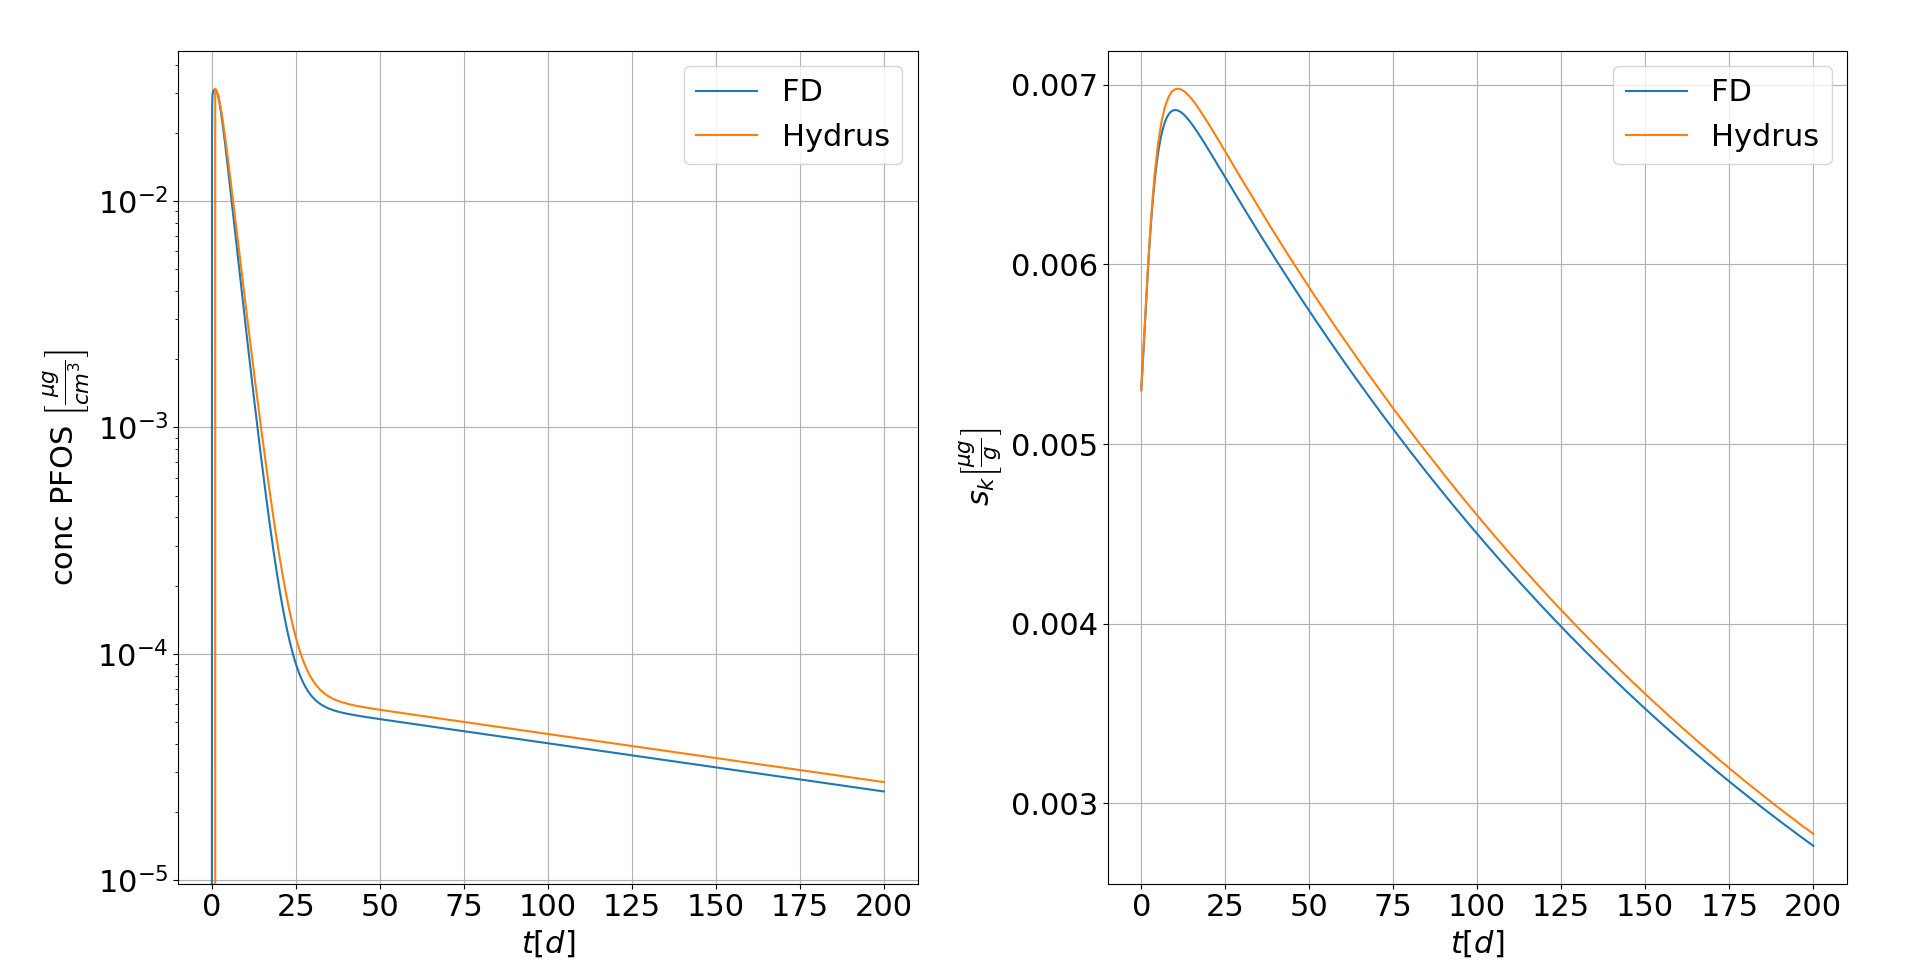
\includegraphics[width=\textwidth]{images/hyd_fd_last_cell_sand.png}
\caption[Comparison of Hydrus and FD BTC with sand]{Comparison of Hydrus and FD solution with sand: $c$ in bottom row (left), $s_k$ in bottom contaminated soil row (right), setting with two sand layers.}
\label{fig:hyd_fd_last_cell_sand}
\end{figure}
\FloatBarrier
\section{Learning from Synthetic Data}
With previously, with the FD solver generated synthetic data of $c$ and $s_k$, the learning capability of FINN was demonstrated. The material parameters (Table \ref{tab:mat_pams}) were inspired by work of Bierbaum et al. The model parameters (Table \ref{tab:mod_pams}) were chosen to maximize effects of both instantaneous and kinetic sorption, as well as effects of the Freundlich isotherm, in order to accurately measure FINN's learning ability. Only two days and a relatively rough spatial discretization was chosen to save computational effort (Table \ref{tab:disc_pams}). The number of time steps used, depended on the CFL condition in the sand, was calculated with eq. \ref{eq:CFL}
\begin{equation}
    T_{STEPS} \geq 2 \cdot T_{MAX} \cdot \frac{\alpha_L \cdot \frac{q}{n_e}}{R^*} \cdot \frac{1}{(\frac{X_{LENGTH}}{X_{STEPS}-1})^2} + 1 = 2 \cdot 2 \cdot \frac{5 \cdot \frac{31.56}{0.31}}{1} \cdot \frac{1}{(\frac{55}{28-1})^2} + 1 \approx 492,
\end{equation}
and was chosen with a corresponding margin.
\begin{table}[h!]
    \centering
    \begin{tabular}{h|ccccccc}
     \quad & $n_{e} \left[-\right]$ & $\rho \left[\frac{g}{cm^3}\right]$ & $D_e \left[\frac{cm^2}{d}\right]$ & $\alpha_l \left[cm\right]$ & $c_{init} \left[\frac{\mu g}{cm^3}\right]$ & $s_{k, init} \left[\frac{\mu g}{g}\right]$ & $q \left[\frac{cm}{d}\right]$  \\ [0.2 cm] \hline
     sand & 0.31 & NaN & 0 & 5 & 0 & 0 & 31.56 \\
     soil & 0.4 & 1.58 & 2.5 & 9 & 0.032 & 0.0053 & 31.56 \\
    \end{tabular}
    \caption[Initial material parameters of FINN, learning from synthetic data]{Initial material parameters of FINN, used for learning from synthetic data.}
    \label{tab:mat_pams}
\end{table}
\begin{table}[h!]
    \centering
\begin{tabular}{h|ccccc}
     \quad & $k_d \left[\frac{cm^3}{d}\right]$ & $\beta \left[-\right]$ & $f \left[-\right]$ & $\alpha_k \left[\frac{1}{d}\right]$ \\ [0.2 cm] \hline
     soil & 1.5 & 0.7 & 0.3 & 0.1
\end{tabular}
    \caption[Initial model parameters of FINN, learning from synthetic data]{Initial model parameters of FINN, used for learning from synthetic data.}
    \label{tab:mod_pams}
\end{table}
\begin{table}[h!]
    \centering
\begin{tabular}{cccccc}
      $T_{MAX} \left[d\right]$ & $T_{STEPS} \left[-\right]$ & $X_{LENGTH} \left[cm\right]$ & $X_{STEPS} \left[-\right]$ & top & bot \\ [0.2 cm] \hline
      2 & 600 & 55 & 28 & 4 & 24
\end{tabular}
    \caption[Initial discretization parameters of FINN, learning from synthetic data]{Initial discretization parameters of FINN, used for learning from synthetic data.}
    \label{tab:disc_pams}
\end{table}
\FloatBarrier
\subsection{Learning Parameters}
\textbf{Run a: Learn Dummy Parameter}\\
In order to validate the FV method added to FINN, all parameters and functional relations are first known and correspond to those from the FD solver. Technically, in order to not receive error messages in the optimizer in Pytorch, a dummy parameter must be added, that does not change the solution, but is considered in the dynamic computational graph. Here, a parameter with value 0 was added in the \texttt{flux\_kernel} when calculating $\mathcal{R}(\varphi_{\mathcal{A}}(c_i))$ on $f_{i+}$, since this is also always 0 due to the positive $v$.\\
The MSE of the entire FINN solution with respect to the entire FD solution was used to calculate the loss (Tab. \ref{table:dummy}, Fig.  \ref{fig:res_ov_synt_dummy}). Deviations only occured at specific points, but in its entirety the differences of $c_{FD}$ and $c_{FINN}$, and $s_{k, FD}$ and $s_{k, FINN}$ fluctuated around zero (Fig. \ref{fig:res_diff_synt_dummy}). The MSE corresponds to machine accuracy. The FV method added to FINN thus produces the same results as the FD solver.
\begin{table}[]
    \centering
    \begin{tabular}{c|ccc|cc|c}
    run a & \multicolumn{3}{c}{Parameters}& \multicolumn{3}{c}{Learning schedule}\\
          learn & ref & init & predicted & epochs & lr & MSE \\[0.2 cm] \hline
         dummy & 0 & 0 & 0 & 1 & 0.1 & $5.2 \times 10^{-19}$\\
    \end{tabular}
    \caption{FINN pass with dummy parameter, run a.}
    \label{table:dummy}
\end{table}
\begin{figure}[]
	\centering
	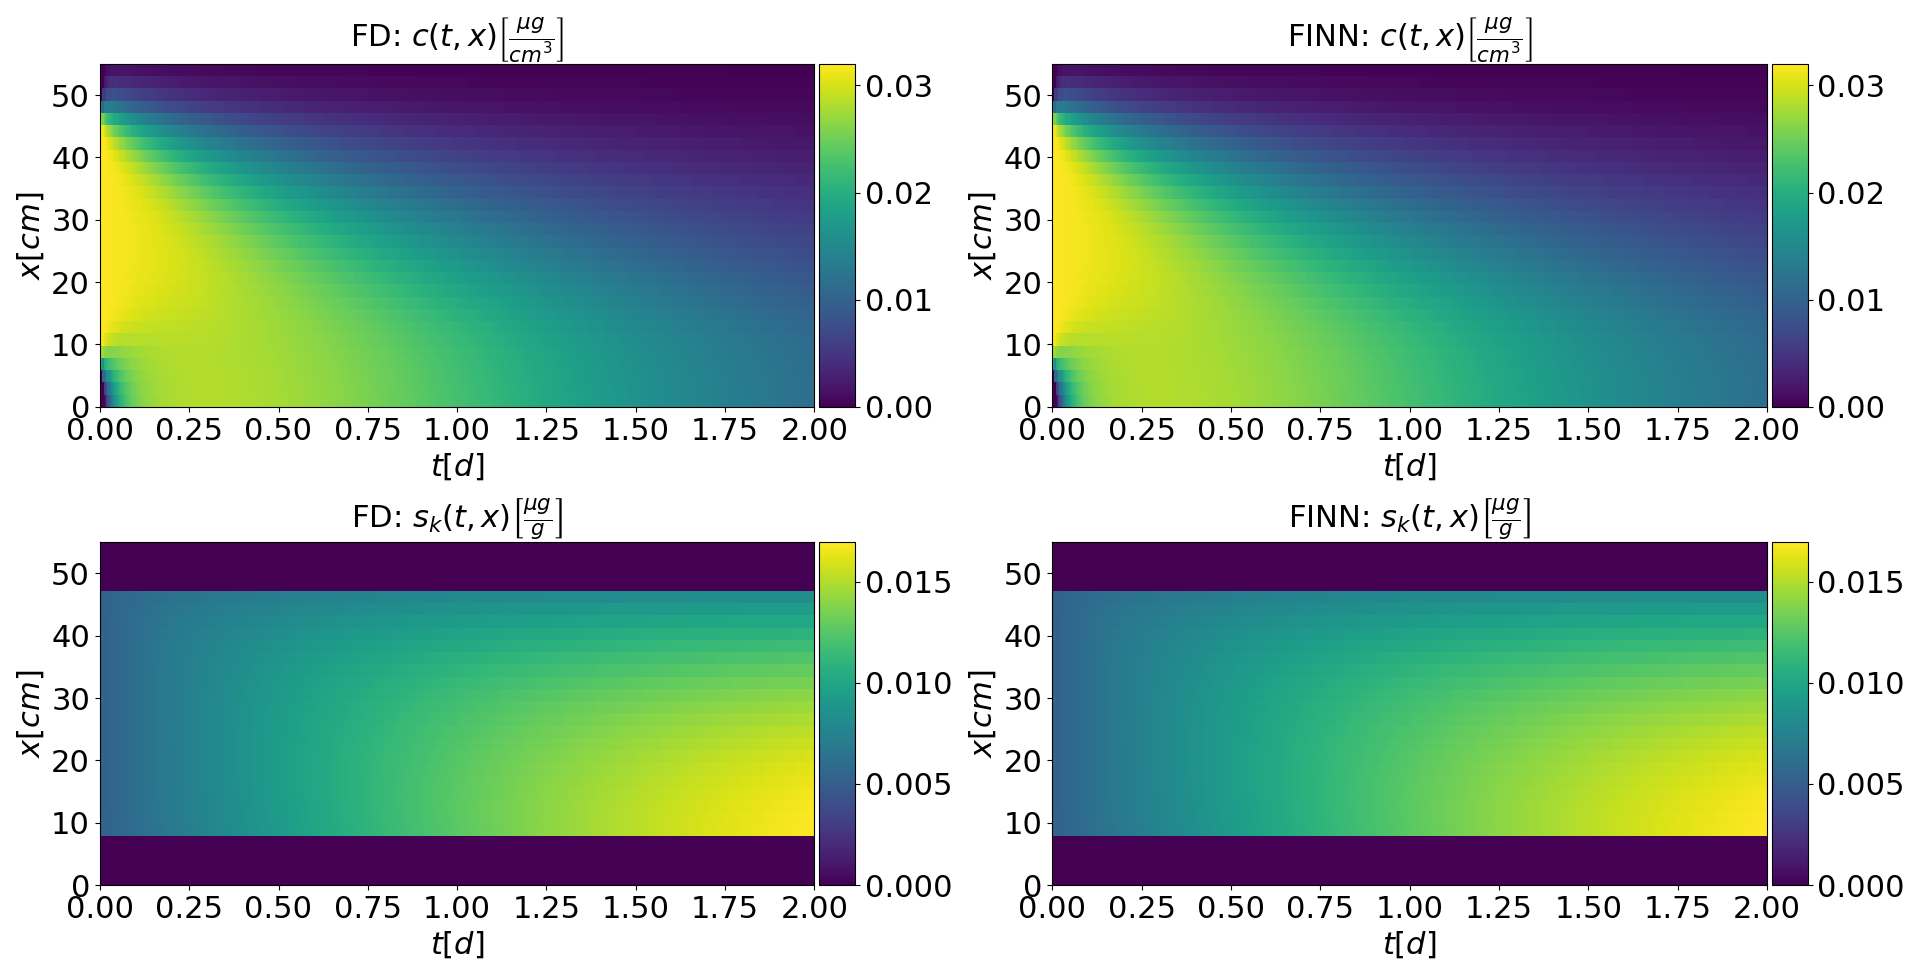
\includegraphics[width=\textwidth]{images/res_ov_synt_dummy.png}
\caption[Comparison of FD and FINN solution, run a]{Comparison of FD and FINN solution, run a.}
\label{fig:res_ov_synt_dummy}
\end{figure}
\begin{figure}[]
	\centering
	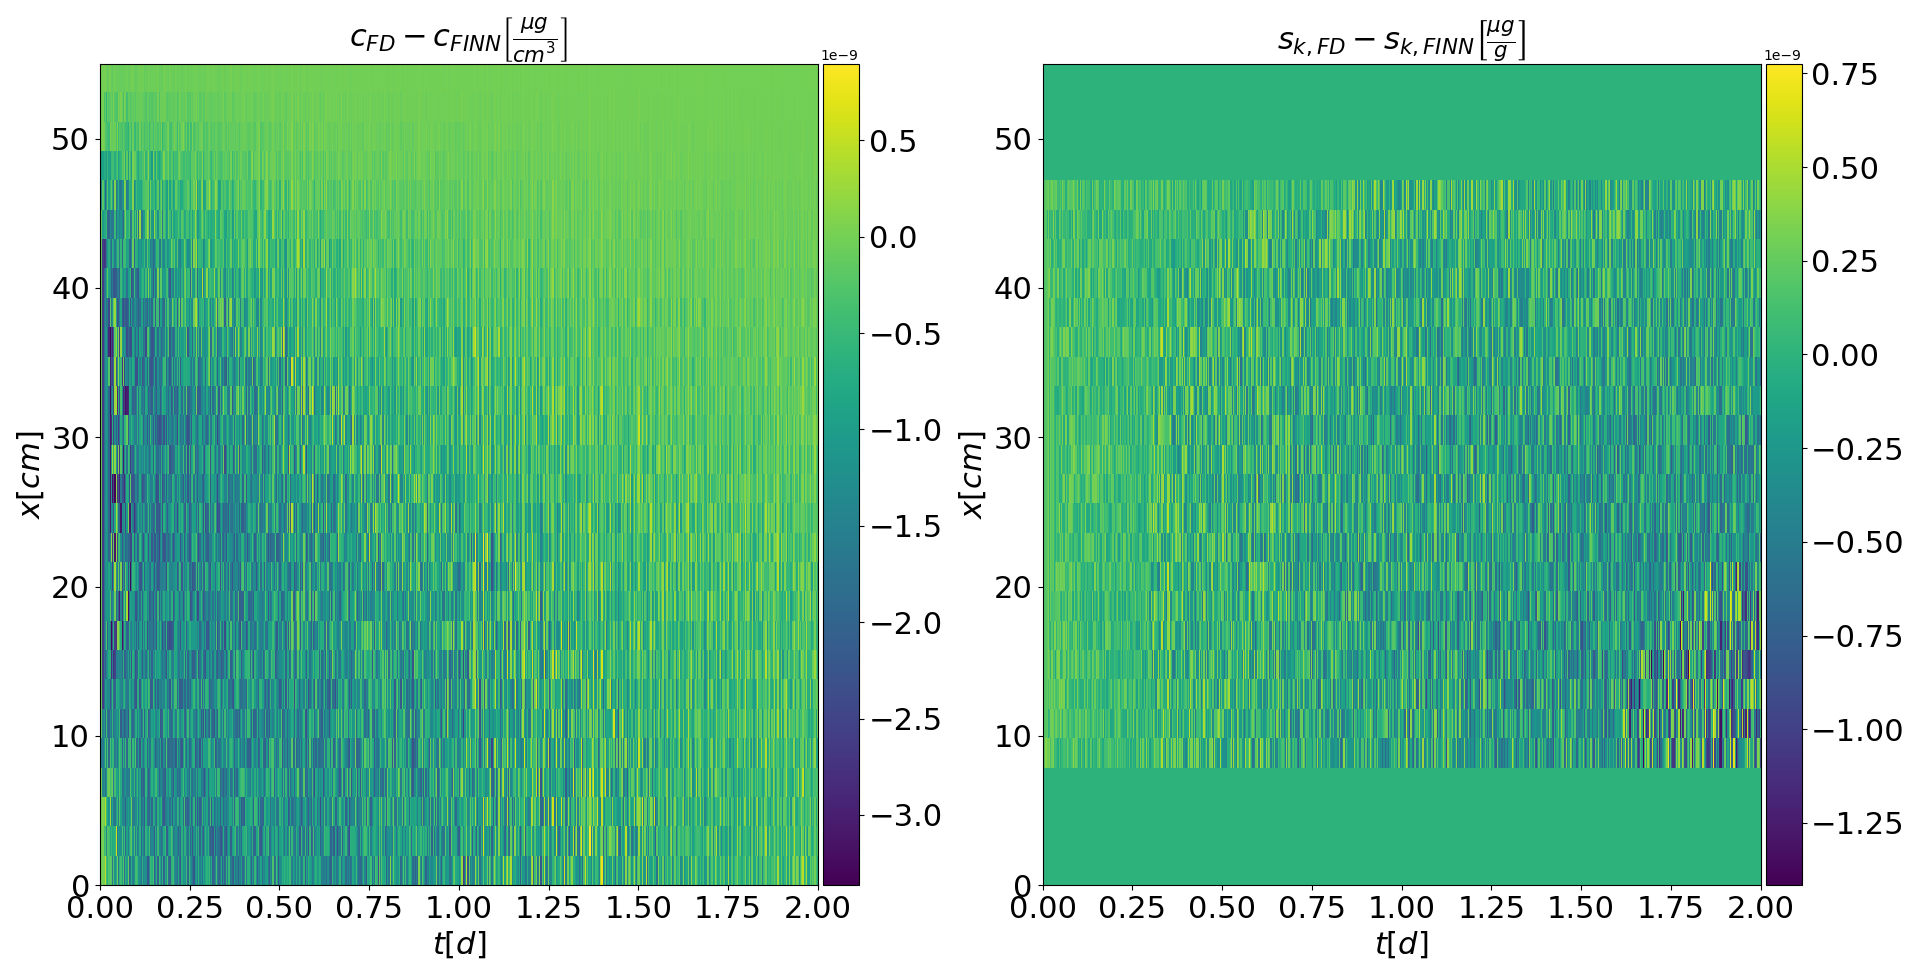
\includegraphics[width=\textwidth]{images/res_diff_synt_dummy.png}
\caption[Difference of FD and FINN solution, run a]{Differences of FD and FINN solution, run a.}
\label{fig:res_diff_synt_dummy}
\end{figure}
\FloatBarrier
\\
\\
\textbf{Run b: Learn $f$}
\\
In order to test FINN's optimization ability the parameter $f$ was included by an initial guess and set as learnable (Tab. \ref{table:learn_f}, Figs. \ref{fig:res_ov_synt_pf}, \ref{fig:res_diff_synt_pf}, \ref{fig:res_btc_synt_pf}, \ref{fig:res_sorp_synt_pf}). With the described learning schedule $f$ was approximated exactly. The MSE corresponds again to machine accuracy.
\begin{table}[h!]
    \centering
    \begin{tabular}{c|ccc||ccc}
         run b& \multicolumn{3}{c}{Parameters}& \multicolumn{3}{c}{Learning schedule} \\
          learn & ref & init & predicted & epochs & lr & MSE \\[0.2 cm] \hline
         $f[-]$ & 0.3 & 0.7 & 0.3 & 20 & 0.1 & $4.18 \times 10^{-7}$ \\
         \quad & \quad & \quad & \quad & 20 & 0.01 & $2.61 \times 10^{-10}$\\
         \quad & \quad & \quad & \quad & 10 & 0.001 & $2.02 \times 10^{-13}$\\
         \quad & \quad & \quad & \quad & 10 & 0.0001 & $6.79 \times 10^{-18}$\\
    \end{tabular}
    \caption[FINN pass with unknown $f$, run b]{FINN pass with unknown $f$, ref denotes the $f$ used in the FD solver which was used to obtain the synthetic training data, init denotes the initial guess for $f$ of FINN, predicted denotes the value of $f$ after optimization. In total 60 epochs were executed with the described learning schedule, run b.}
    \label{table:learn_f}
\end{table}
\FloatBarrier
\\
\\
\textbf{Run c: Learn $f$, $k_d$, $\beta$, $\alpha_k$}
\\
All model parameters $f$, $k_d$, $\beta$ and $\alpha_k$ were learnable in run c and included by initial guesses (Tab. \ref{tab:learn_f_k_d_beta_alpha_k}, Fig. \ref{fig:res_ov_synt_pparam}). With the described learning schedule the parameters were approximated well. Using the high amount of epochs the MSE is again close to machine accuracy. Deviations in the differences occured because the approximated parameters did not yet correspond exactly to the initial parameters (Fig. \ref{fig:res_diff_synt_pparam}). In order to visualize the deviations between the FINN and FD solution at fixed time steps, $c$ and $s_k$ of the entire contaminated soil layer were plotted.  These $c$ - $s_k$ sorption isotherms were approximated well (Fig. \ref{fig:res_sorp_synt_pparam}). Additionaly the BTC (Fig. \ref{fig:res_btc_synt_pparam}, left) and $s_k$ at $t=2.0d$ over the column length (Fig. \ref{fig:res_btc_synt_pparam}, right) were visualized. Because of very close approximation of the parameters to the reference values, these courses were approximated well too. As expected with decreasing column length $s_k$ is increasing. $s_k$ accumulates at the bottom of the contaminated soil layer. Thus, for the entire simulation period $(1-f)k_dc^\beta > s_k$.
\begin{table}[h!]
    \centering
    \begin{tabular}{c|ccc||cc|c}
    run c & \multicolumn{3}{c}{Parameters}& \multicolumn{3}{c}{Learning schedule}\\
          learn & ref & init & predicted(*) & epochs & lr & MSE \\[0.2 cm] \hline
         $f[-]$ & 0.3 & 0.8 & 0.300096 & 10 & 0.1 & $5.13 \times 10^{-5}$\\
         $k_d \left[\frac{cm^3}{d}\right]$ & 1.5 & 2 & 1.499331 & 300 & 0.01 & $2.99 \times 10^{-8}$\\
          $\beta \left[-\right]$ & 0.7 & 0.5 & 0.699951 & 8000 & 0.001 & $7.52 \times 10^{-15}$\\
         $\alpha_k \left[\frac{cm}{d}\right]$ & 0.1 & 0.6 & 0.100046 & & & \\
    \end{tabular}
    \caption[FINN pass with learnable $f$, $k_d$, $\alpha_k$, $\beta$, run c]{FINN pass with learnable $f$, $k_d$, $\alpha_k$, $\beta$, (*) values rounded at 6th digit after decimal point, run c.}
    \label{tab:learn_f_k_d_beta_alpha_k}
\end{table}
\begin{figure}[h!]
    \centering
    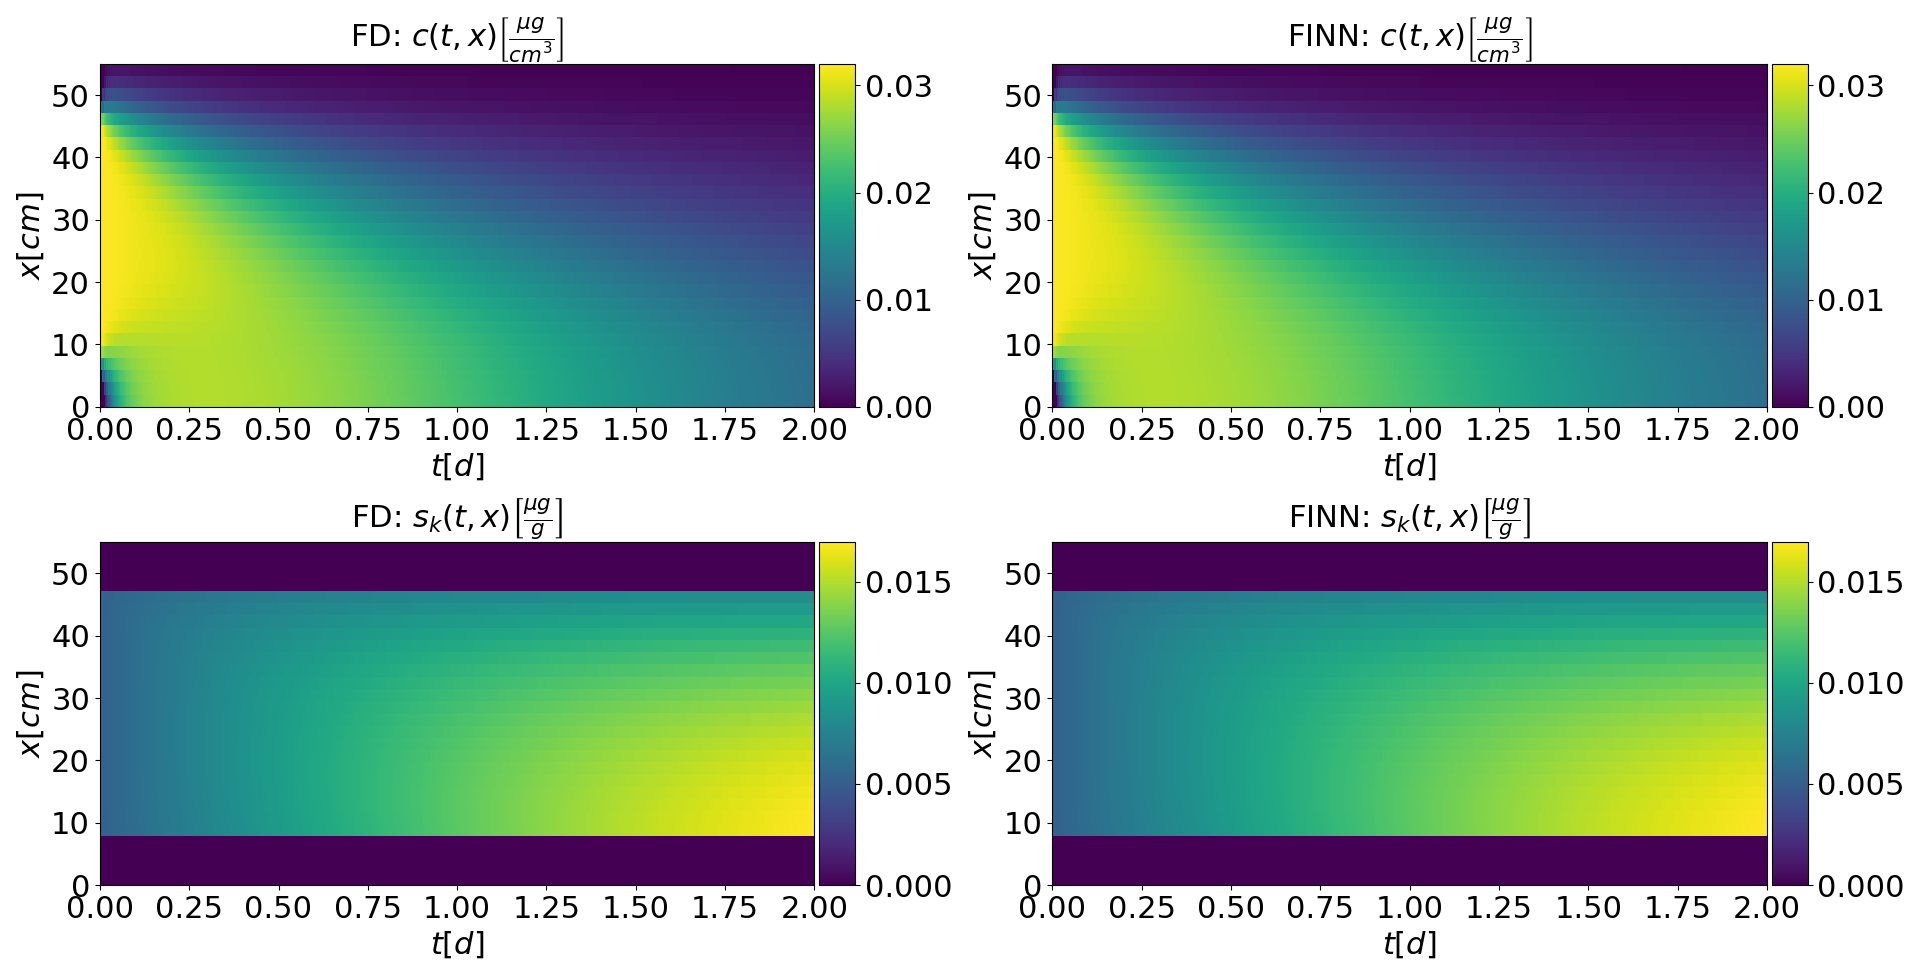
\includegraphics[width=\textwidth]{images/res_ov_synt_pparam.png}
    \caption[Comparison of FD and FINN solution, run c]{Comparison of FD and FINN solution, run c.}
    \label{fig:res_ov_synt_pparam}
\end{figure}
\begin{figure}[h!]
    \centering
    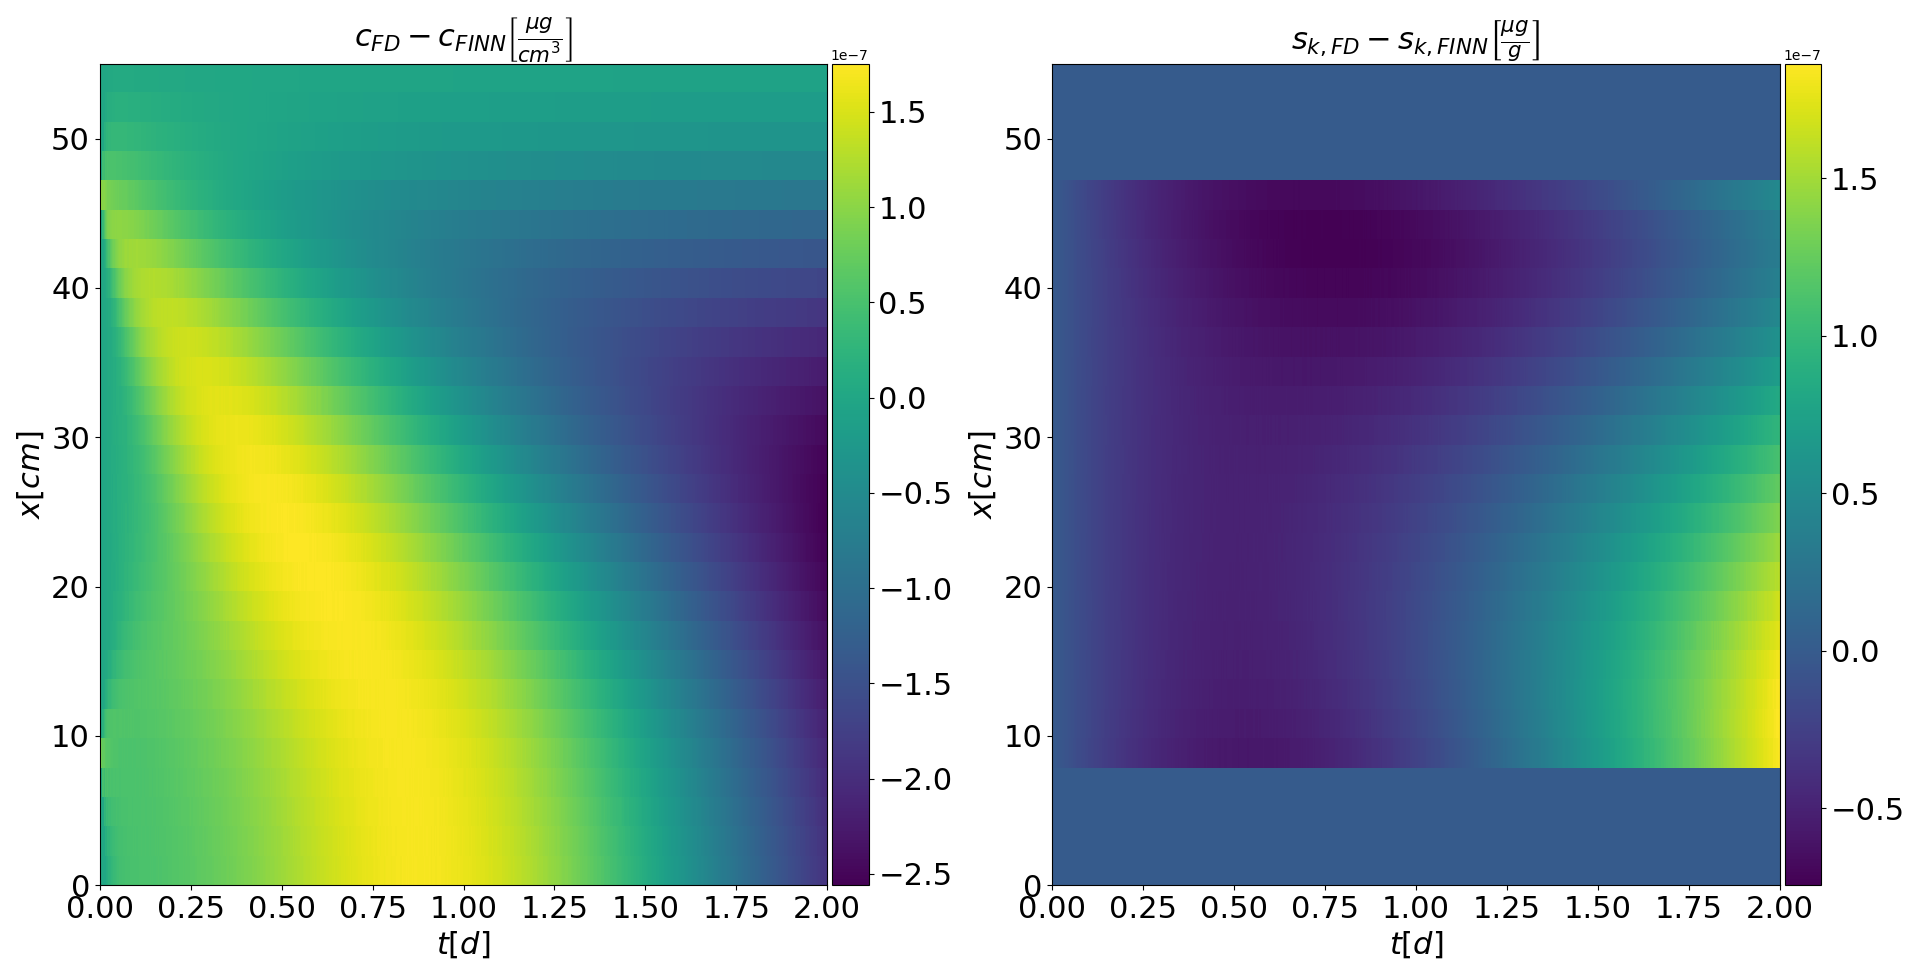
\includegraphics[width=\textwidth]{images/res_diff_synt_pparam.png}
    \caption[Difference of FD and FINN solution, run c]{Difference of FD and FINN solution, run c.}
    \label{fig:res_diff_synt_pparam}
\end{figure}
\begin{figure}[h!]
    \centering
    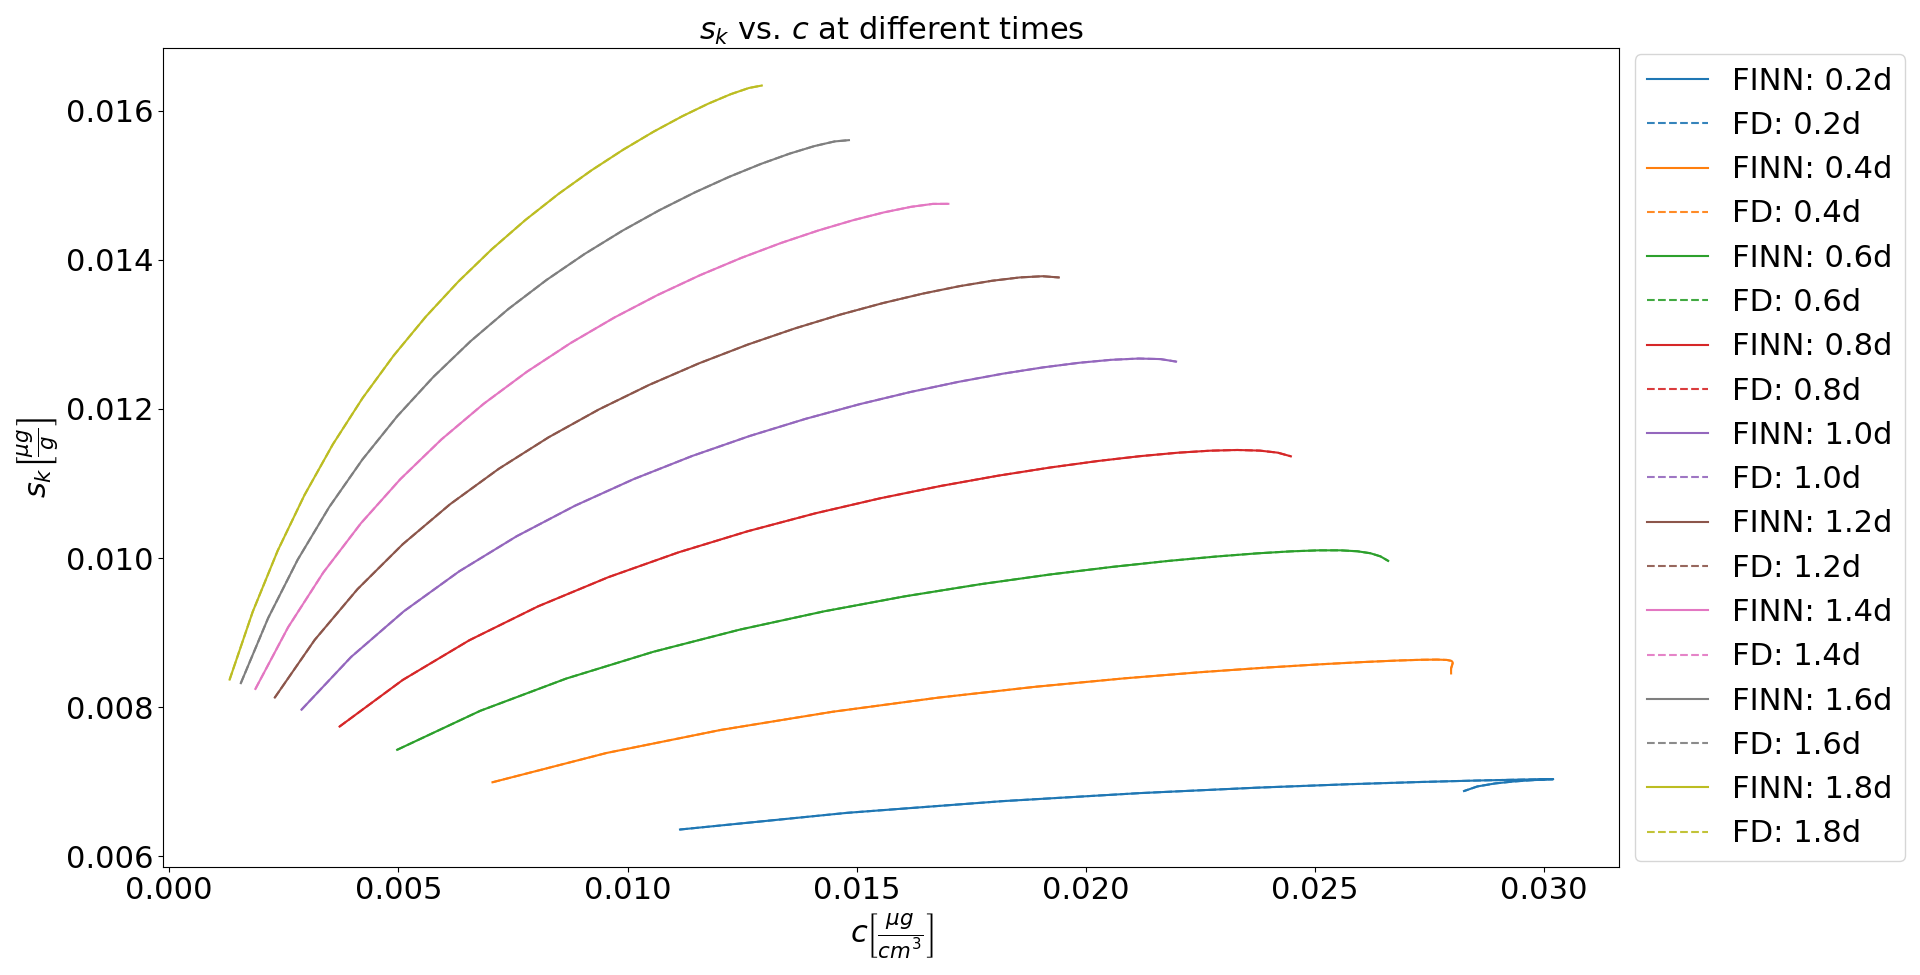
\includegraphics[width=\textwidth]{images/res_sorp_synt_pparam.png}
    \caption[Comparison of FD and FINN sorption behavior, run c]{Comparison of FD and FINN solution: The unknowns $s_k$ and $c$ plotted at fixed time steps, run c.}
    \label{fig:res_sorp_synt_pparam}
\end{figure}
\begin{figure}[h!]
    \centering
    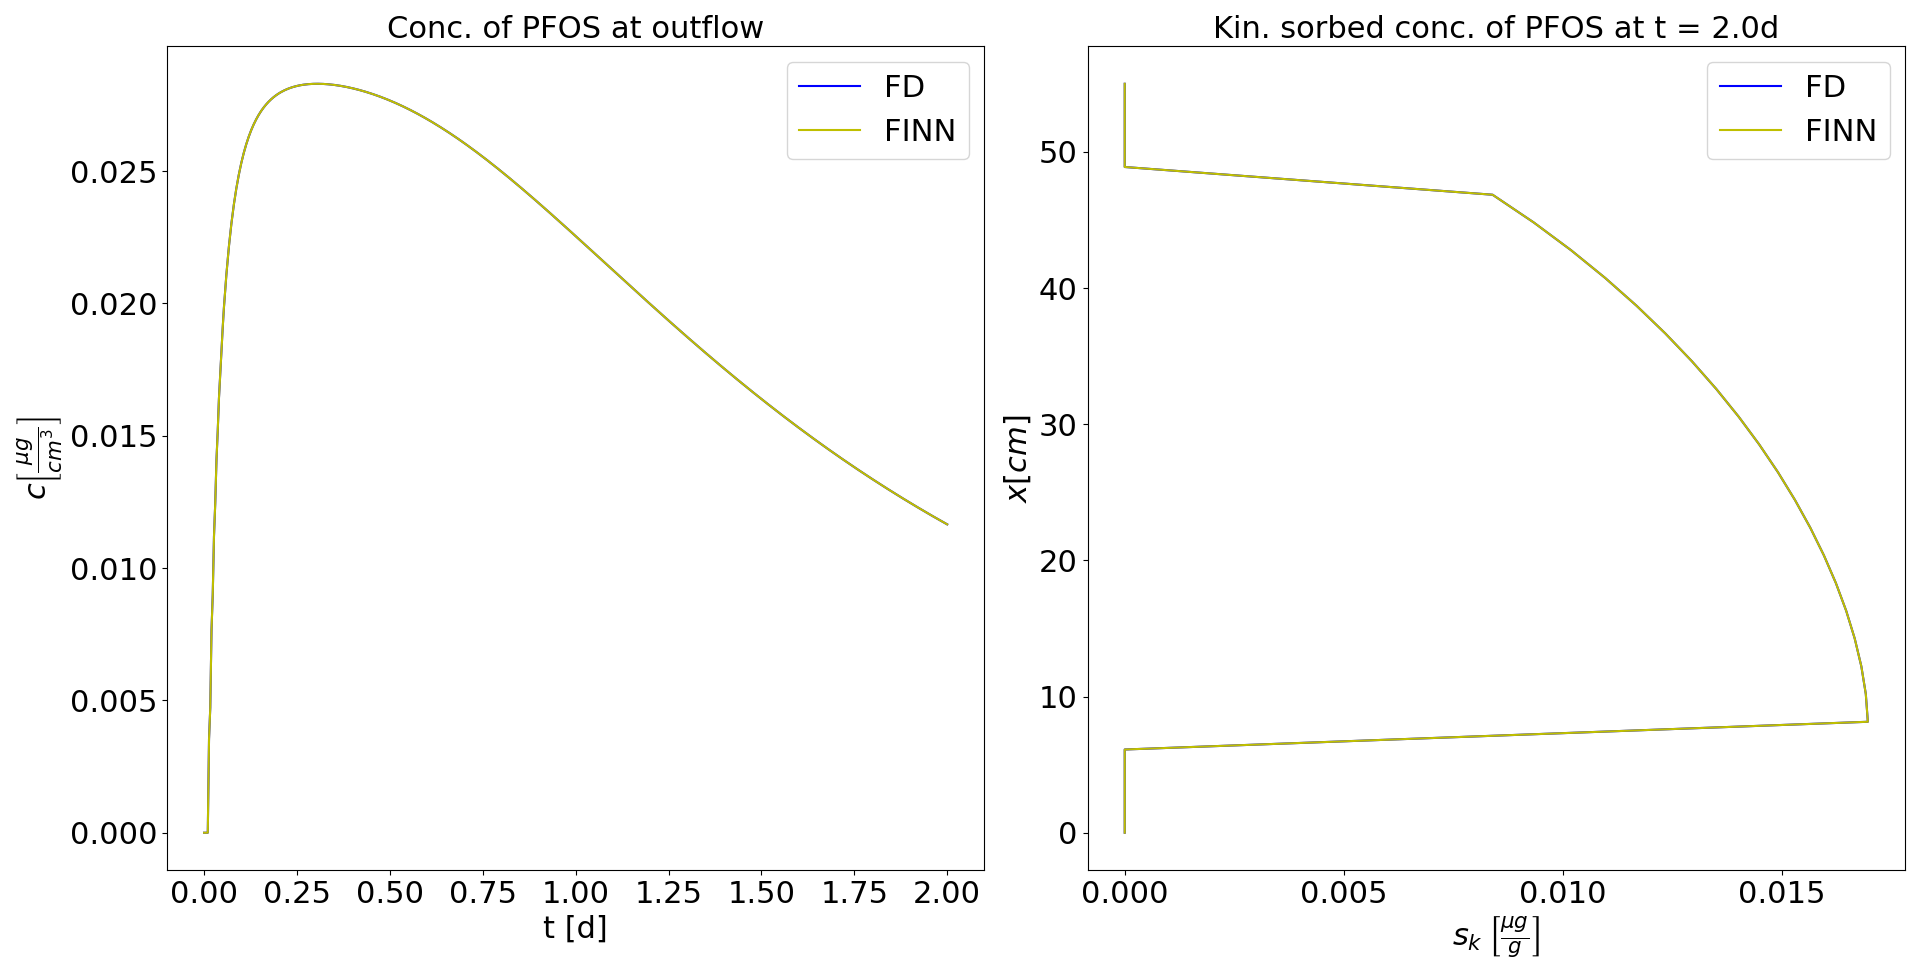
\includegraphics[width=\textwidth]{images/res_btc_synt_pparam.png}
    \caption[Comparison of FD and FINN BTC, run c]{Comparison of FD and FINN solution: BTC of PFOS given by FD and approximated by FINN (left), $s_k$ of PFOS at $t_{end}$ (right), run c.}
    \label{fig:res_btc_synt_pparam}
\end{figure}
\FloatBarrier
\subsection{Learning Functional Relations}
FINN was trained based on synthetic data for $0.5d$ and then tested with the remaining $t = 1.5d$, which is an \textit{in-dis-test}. Each function $F$, $G$ and $R$ was approximated by a time-dependent DNN with two input features, one output feature, and three hidden layers with 20-40-20 neurons respectively. Thus, with biases and scaling term
\begin{equation}
   \#\theta = \underbrace{2 \cdot 20 + 20 \cdot 40 + 40 \cdot 20 + 20 \cdot 1}_{weights} + \underbrace{20 + 40 + 20 + 1}_{biases} + \underbrace{1}_{scale} = 1742
\end{equation}
parameters were used per function.
\\
\\
\textbf{Run d: Learn Time-dependent $F$}
\\
FINN produced good results learning only the function $F$ described in eq. \ref{eq:F}, (Tab. \ref{tab:learn_F}, Fig. \ref{fig:res_ov_synt_F_m}). The loss value after training was two orders of magnitude smaller than the loss value of the test. At time points greater than $t = 0.5d$, the difference between the FD solution and the FINN prediction increased. $s_{k,FD}$ is greater than $s_{k,FINN}$ for the entire simulation time, thus $c_{FD}$ is smaller than $c_{FINN}$, since more PFOS is in kinetically sorbed phase (Fig. \ref{fig:res_diff_synt_F_m}).
\begin{table}[h!]
    \centering
    \begin{tabular}{c|c|cccc}
    run d & init & \multicolumn{4}{c}{Learning schedule} \\
          learn & scalings & epochs & lr & $MSE_{train}$ & $MSE_{test}$\\[0.2 cm] \hline
         $F$ & $f_{sc} = 0.1$ & 300 & 0.01 & $4.42 \times 10^{-9}$ & $1.94 \times 10^{-7}$
        \end{tabular}
    \caption[FINN training and testing with unknown $F$, run d]{FINN training and testing with unknown $F$, run d.}
    \label{tab:learn_F}
\end{table}
\begin{figure}[h!]
	\centering
	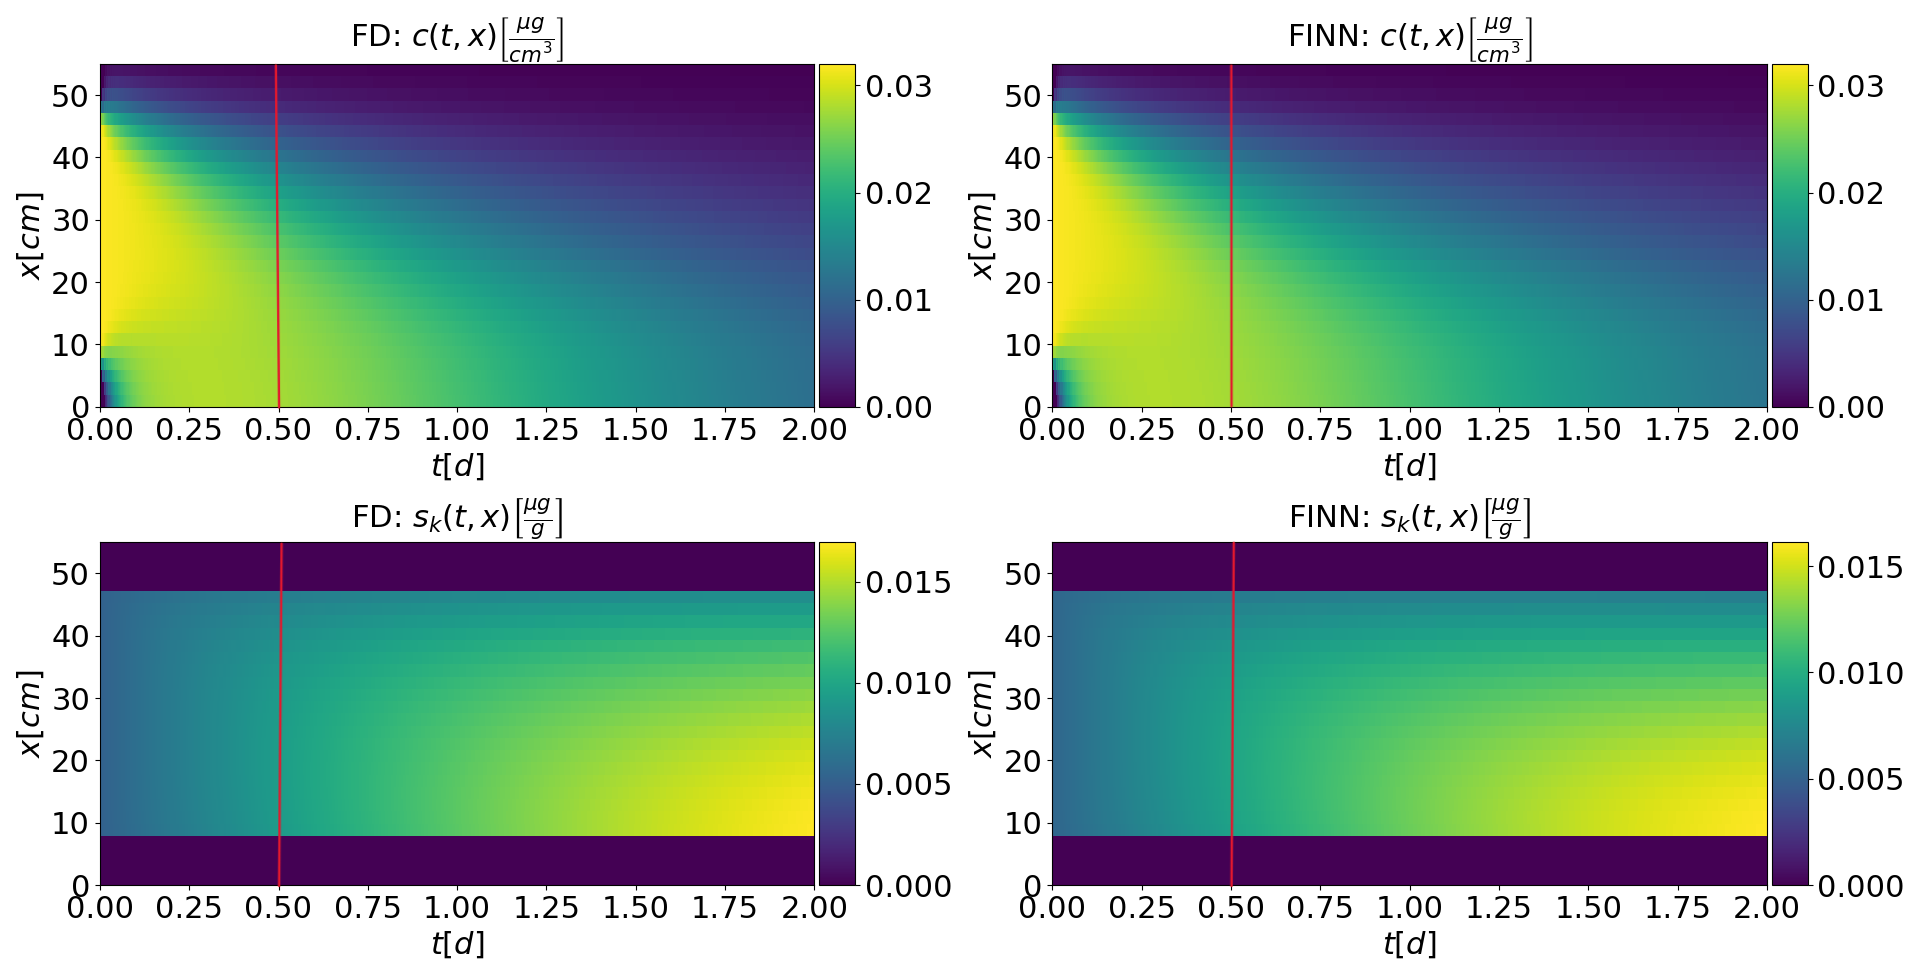
\includegraphics[width=\textwidth]{images/res_ov_synt_F_m.png}
\caption[Comparison of FD and FINN solution, run d]{Comparison of FD and FINN solution: Red line marks the end of the training data set, run d.}
\label{fig:res_ov_synt_F_m}
\end{figure}
\begin{figure}[h!]
	\centering
	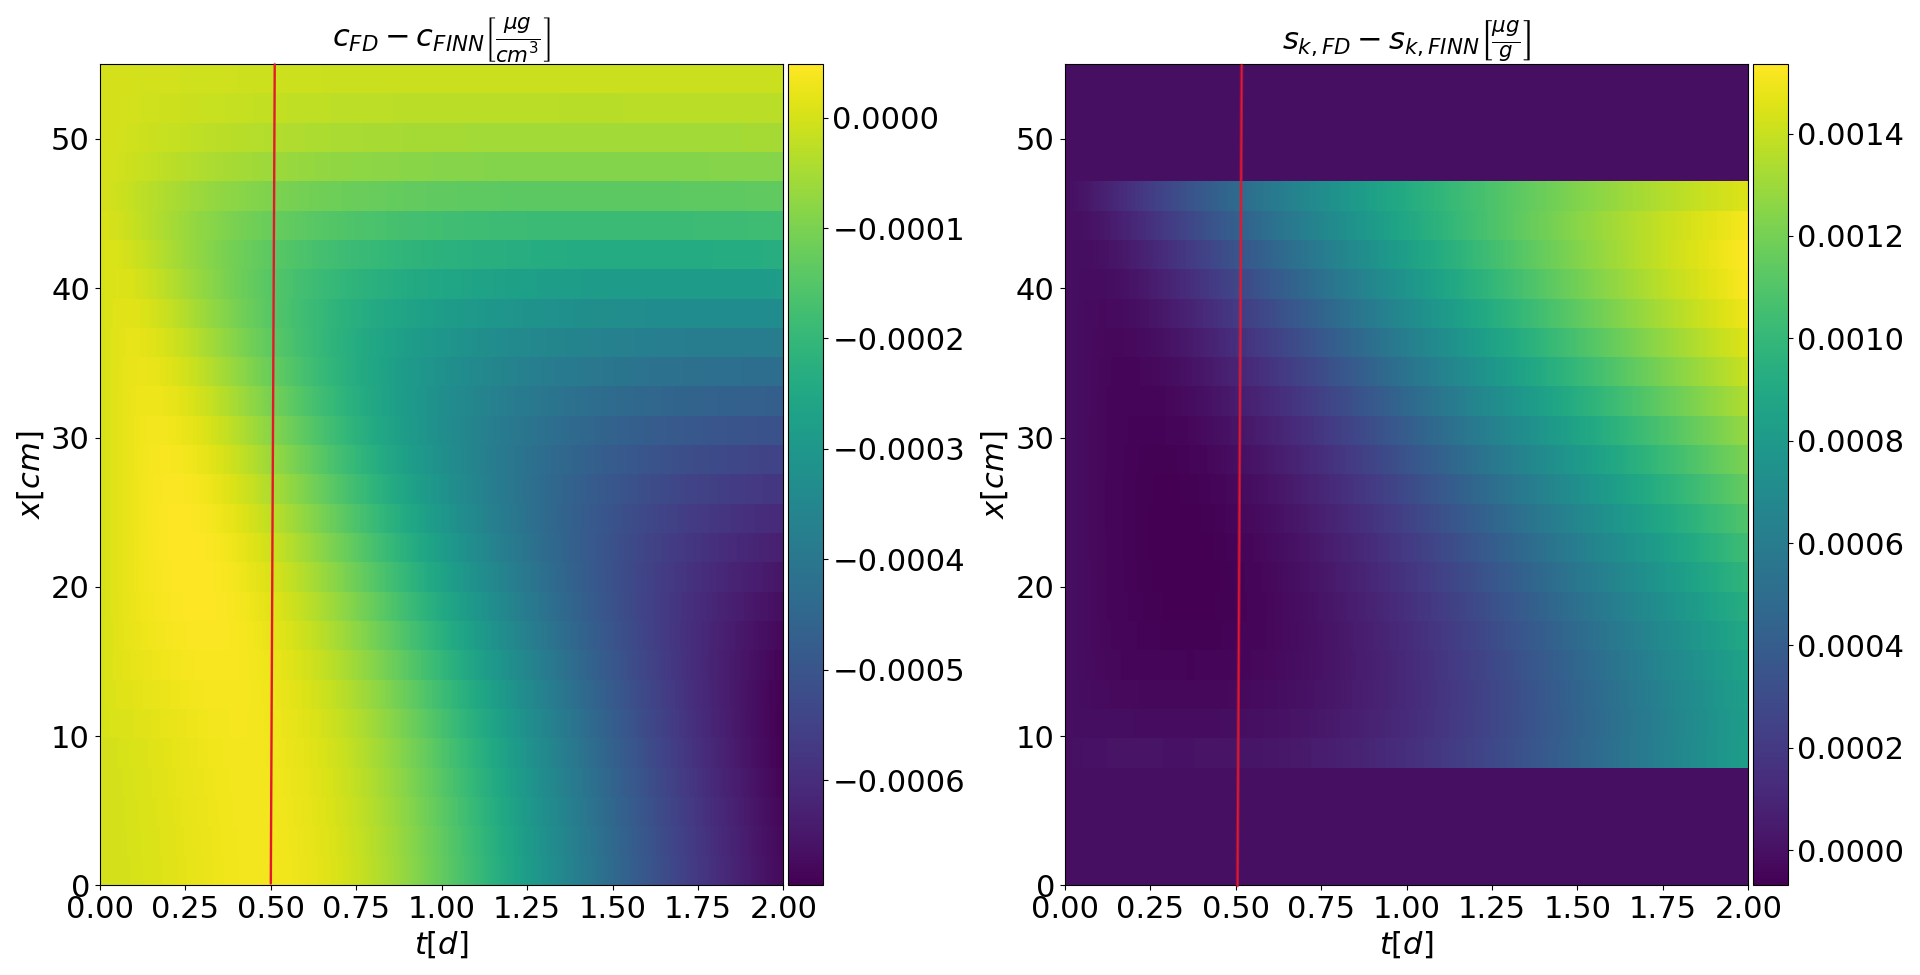
\includegraphics[width=\textwidth]{images/res_diff_synt_F_m.png}
\caption[Difference of FD and FINN solution, run d]{Difference of FD and FINN solution: Red line marks the end of the training data set, run d.}
\label{fig:res_diff_synt_F_m}
\end{figure}\\
The BTC was approximated better in training than in testing. The tested model overestimates $c$ at the outflow. Mass conservation seems to be plausible: In the FINN solution $c$ is larger compared to the FD solution. Thus also the instantaneously sorbed concentration, calculated by the Freundlich sorption isotherm eq. \ref{eq:freundlich} is larger. Hence, $s_k$ predicted by FINN is smaller compared to the FD solution (Fig. \ref{fig:res_btc_synt_F_m}).
\begin{figure}[h!]
	\centering
	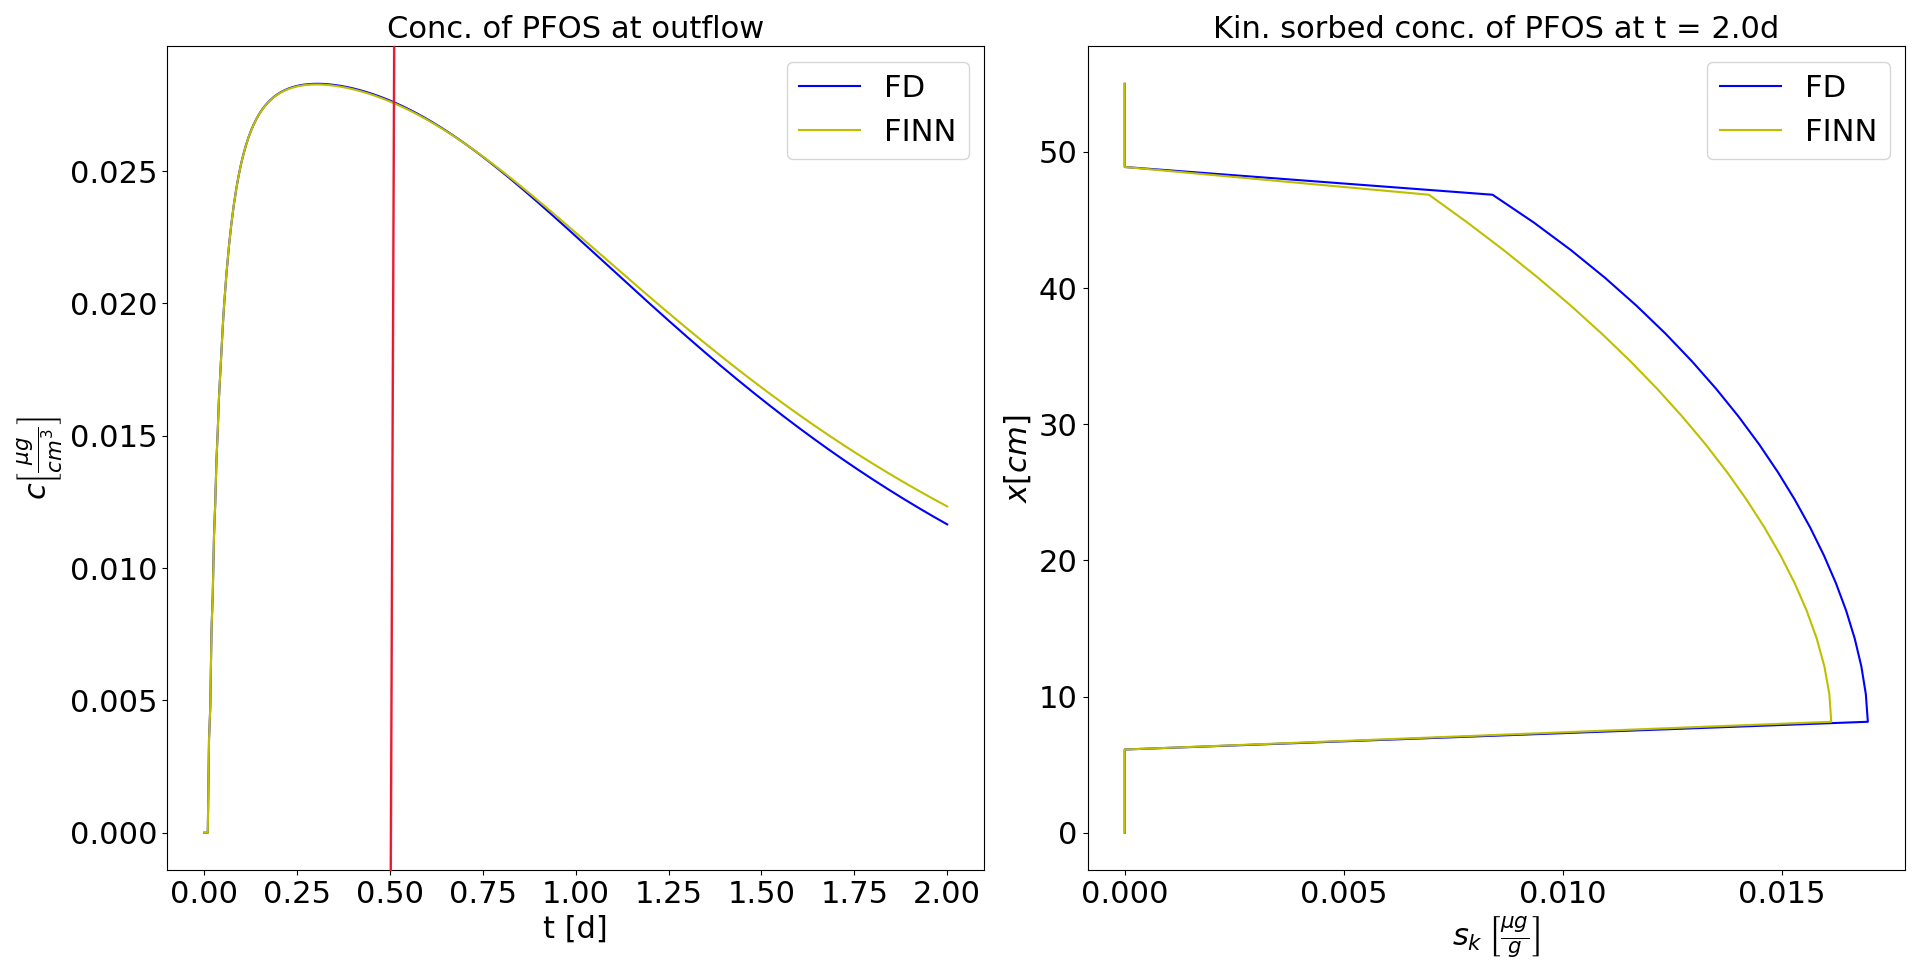
\includegraphics[width=\textwidth]{images/res_btc_synt_F_m.png}
\caption[Comparison of FD and FINN BTC, run d]{Comparison of FD and FINN solution: BTC of PFOS given by FD and approximated by FINN (left), $s_k$ of PFOS at $t_{end}$ (right), run d.}
\label{fig:res_btc_synt_F_m}
\end{figure}\\
The concave course of the $c$ - $s_k$ sorption isotherms in the FD solution was also reproduced by FINN. The sharp edge at $t=0.2d$ is caused by the non-monotonous course of $s_k$ and $c$ over contaminated soil cells. With increasing time, especially at testing time these $c$ - $s_k$ sorption isotherms are predicted worse, due to less $s_k$ in the FINN predicted solution (Fig. \ref{fig:res_sorp_synt_F}).
\begin{figure}
	\centering
	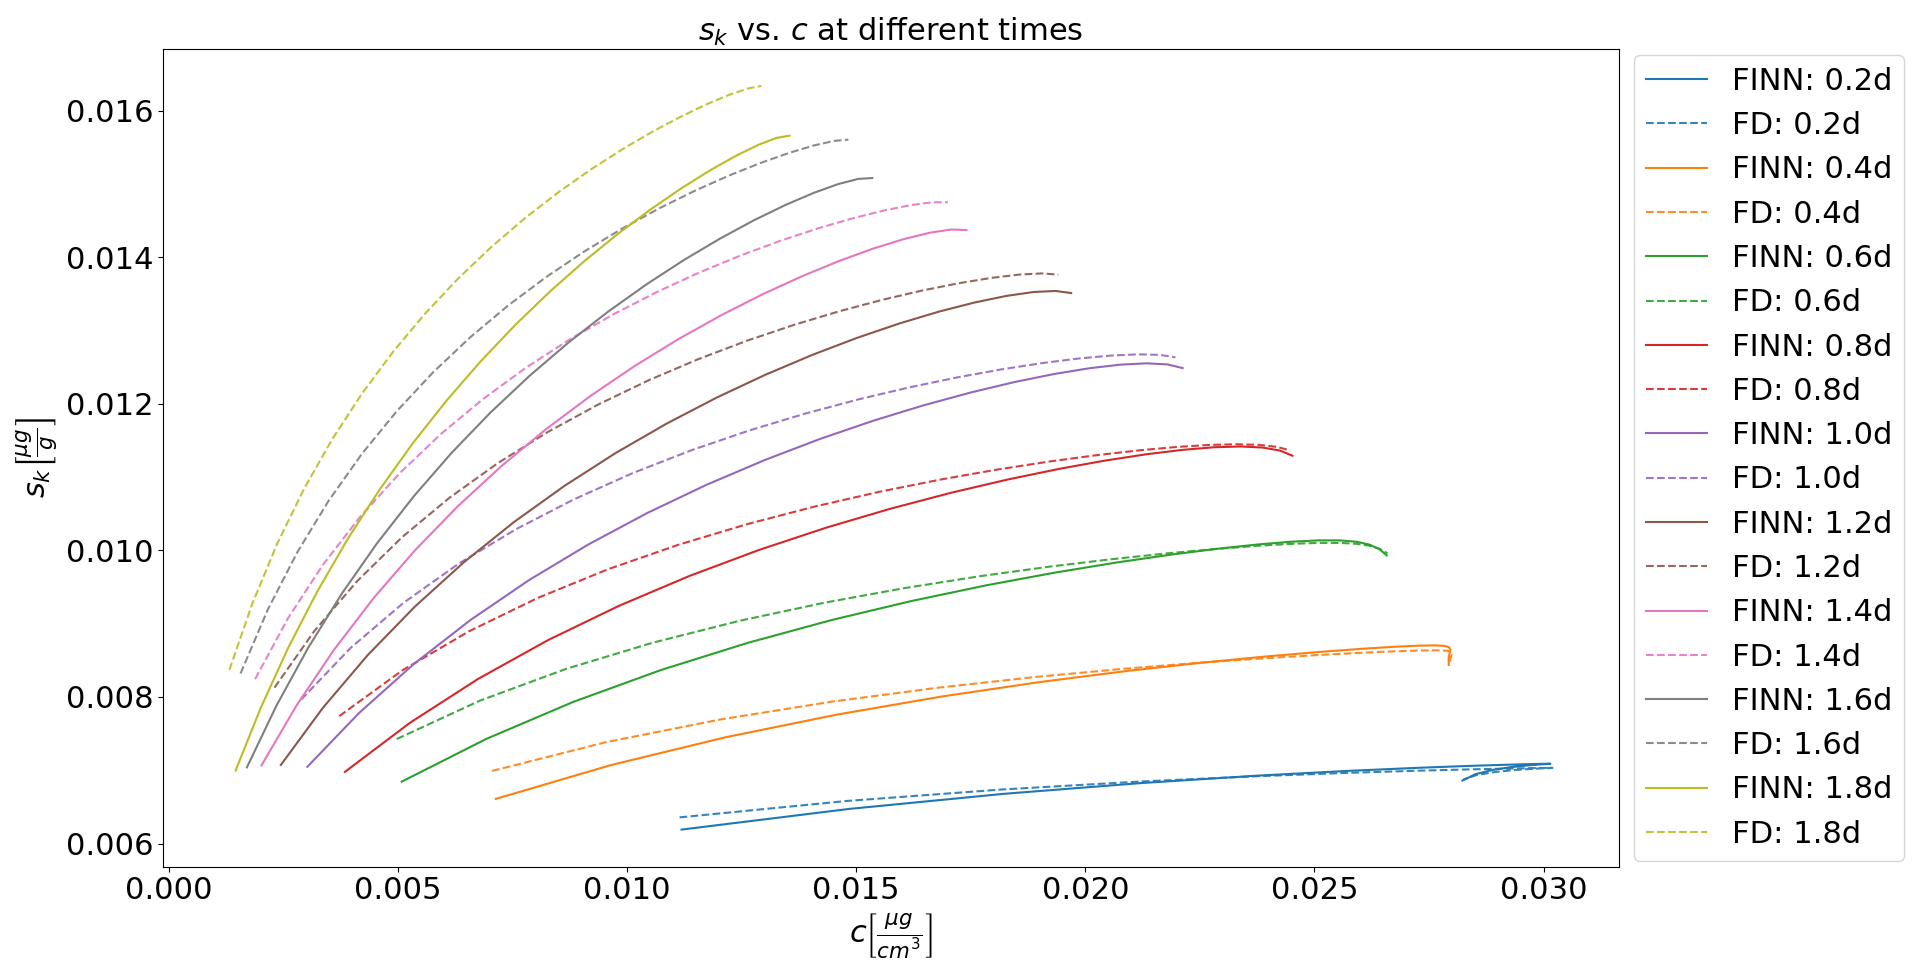
\includegraphics[width=\textwidth]{images/res_sorp_synt_F.png}
\caption[Comparison of FD and FINN sorption behavior, run d]{Comparison of FD and FINN solution: The unknowns $s_k$ and $c$ plotted at fixed time steps, run d.}
\label{fig:res_sorp_synt_F}
\end{figure}
\FloatBarrier
\\
\\
\textbf{Run e: Learn Time-dependent $F$, $G$ and $R$}
\\
In a next step $F$ eq. \ref{eq:F}, $G$ eq. \ref{eq:G} and $R$ eq. \ref{eq:R}, thus the entire sorption process were learned as explicitly time-dependent functions (Tab. \ref{tab:FGR_500}, Fig. \ref{fig:res_ov_synt_FGR_500_m}). The loss values for training and testing were in the same orders of magnitude. Compared to run d the loss after training is two orders of magnitude larger. Probably the model in run d overfitted the data.
\begin{table}[h!]
    \centering
    \begin{tabular}{c|c|cccc}
    run e & init & \multicolumn{3}{c}{Learning schedule}& \\
          learn & scalings & epochs & lr & $MSE_{train}$ & $MSE_{test}$ \\[0.2 cm] \hline
          $F$ & $f_{sc} = 0.1$ & 500 & 0.01 & $5.66 \times 10^{-7}$& \\
          $G$ & $g_{sc} = 0.0001$ & 100&0.001 & $5.49 \times 10^{-7}$ & $8.57 \times 10^{-7}$ \\
          $R$ & $r_{sc} = 1$ & & & & 
        \end{tabular}
    \caption[FINN training with unknown time-dependent functions $F$, $G$, $R$, run e]{FINN training with unknown time-dependent functions $F$, $G$, $R$, run e.}
    \label{tab:FGR_500}
\end{table}
\begin{figure}[h]
	\centering
	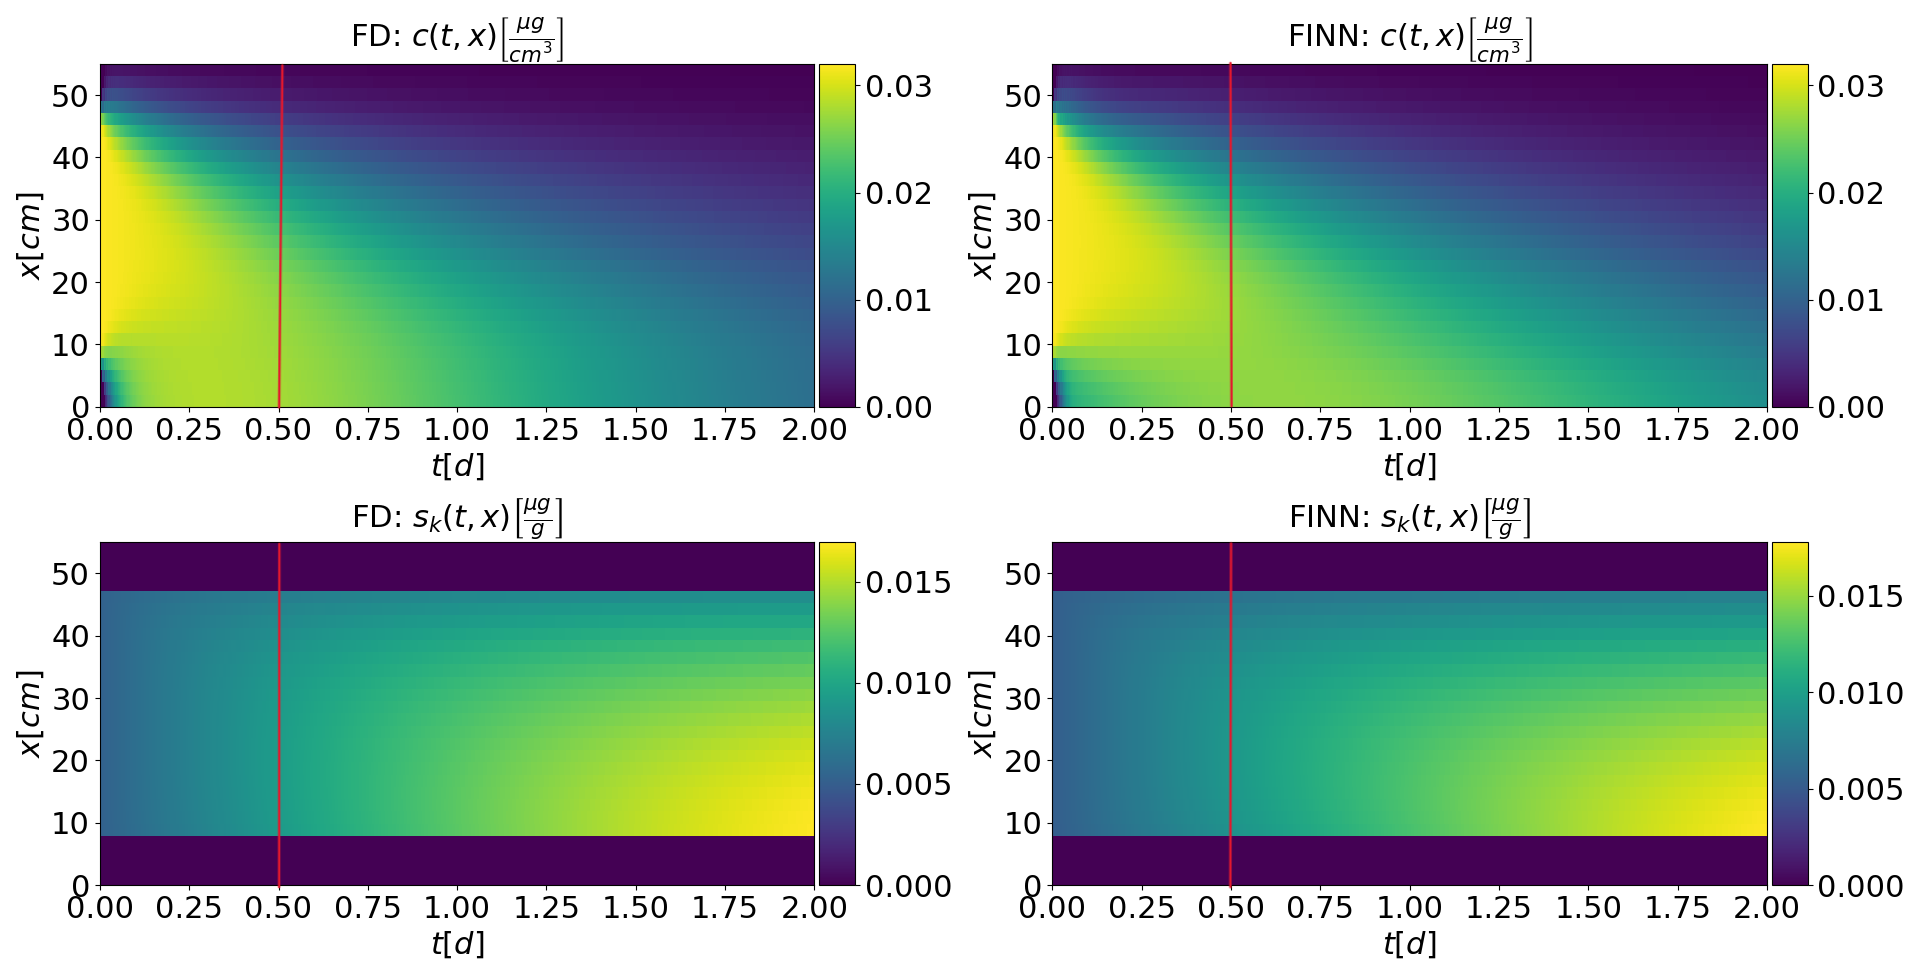
\includegraphics[width=\textwidth]{images/res_ov_synt_FGR_500_m.png}
\caption[Comparison of FD and FINN solution, run e]{Comparison of FD and FINN solution: Red line marks end of the training data set, run e.}
\label{fig:res_ov_synt_FGR_500_m}
\end{figure}
\begin{figure}[h]
	\centering
	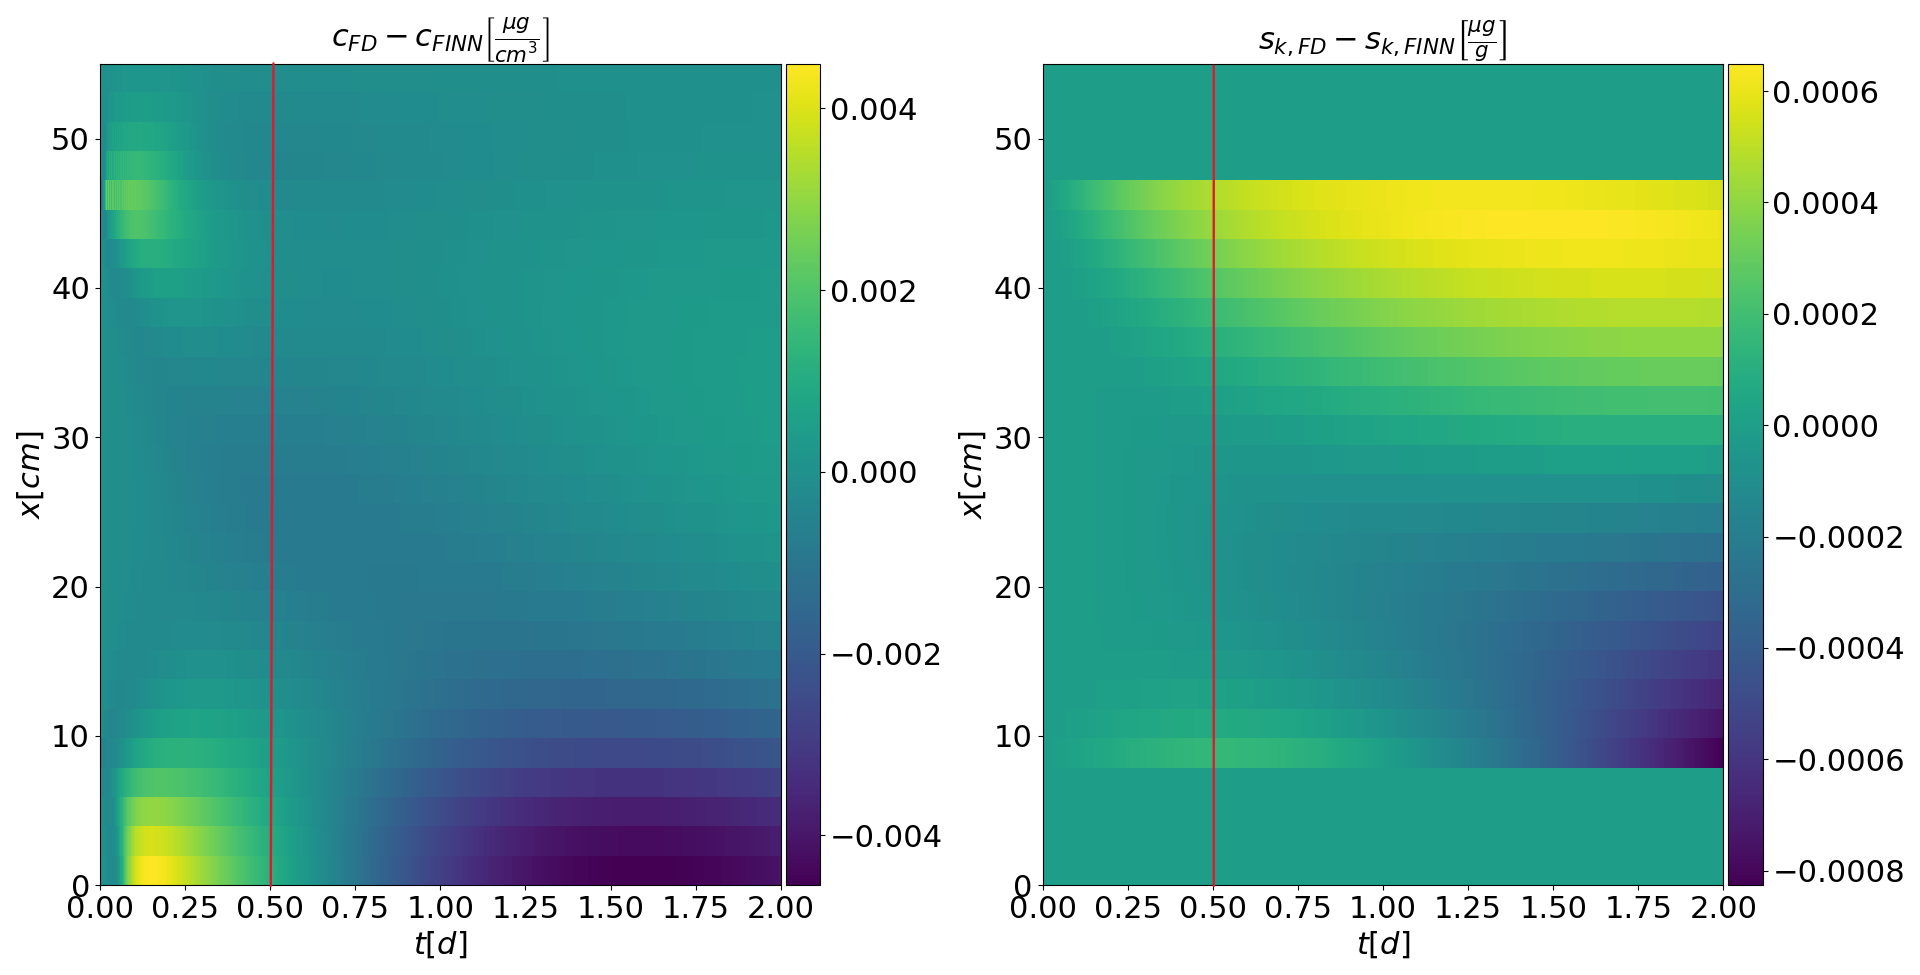
\includegraphics[width=\textwidth]{images/res_diff_synt_FGR_500_m.png}
\caption[Difference of FD and FINN solution, run e]{Difference of FD and FINN solution: Red line marks the end of the training data set, run e.}
\label{fig:res_diff_synt_FGR_500_m}
\end{figure}
\begin{figure}[h]
	\centering
	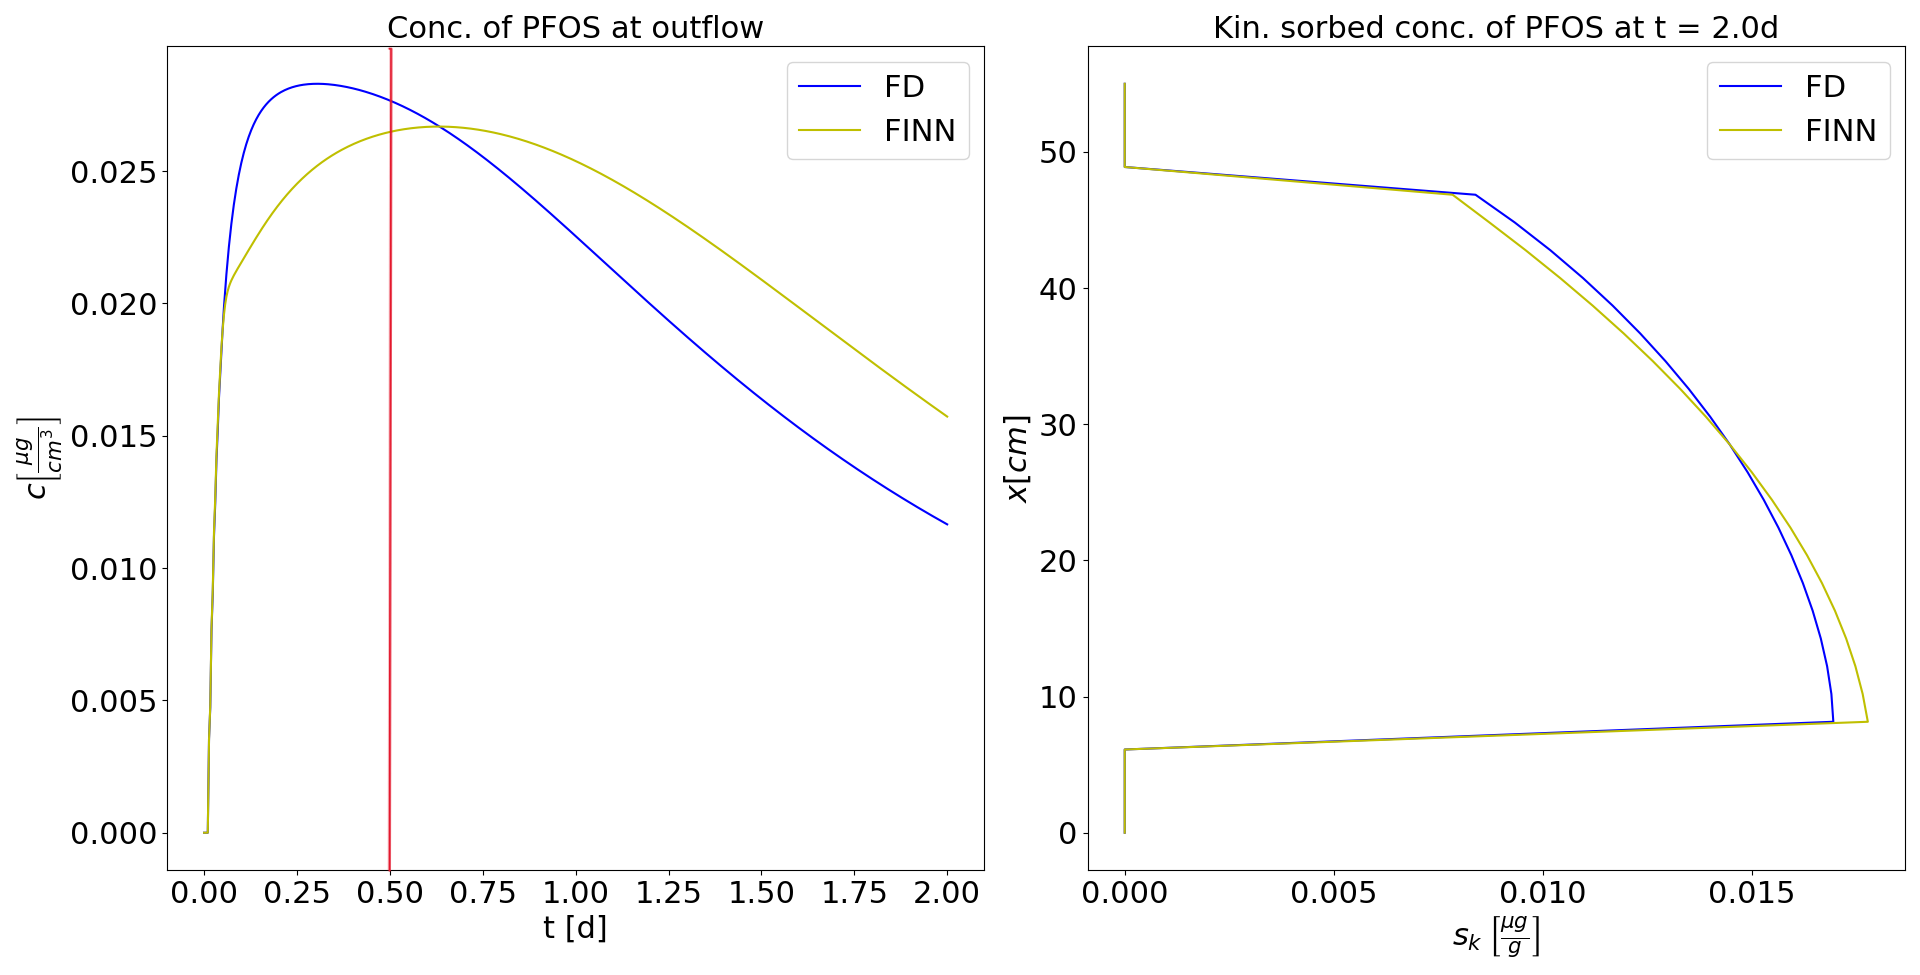
\includegraphics[width=\textwidth]{images/res_btc_synt_FGR_500_m.png}
\caption[Comparison of FD and FINN BTC, run e]{Comparison of FD and FINN solution: BTC of PFOS given by FD and approximated by FINN. Red line marks end of the training data set (left). Kin. sorbed concentration of PFOS at $t_{end}$ (right), run e.}
\label{fig:res_btc_synt_FGR_500_m}
\end{figure}
\begin{figure}[h]
	\centering
	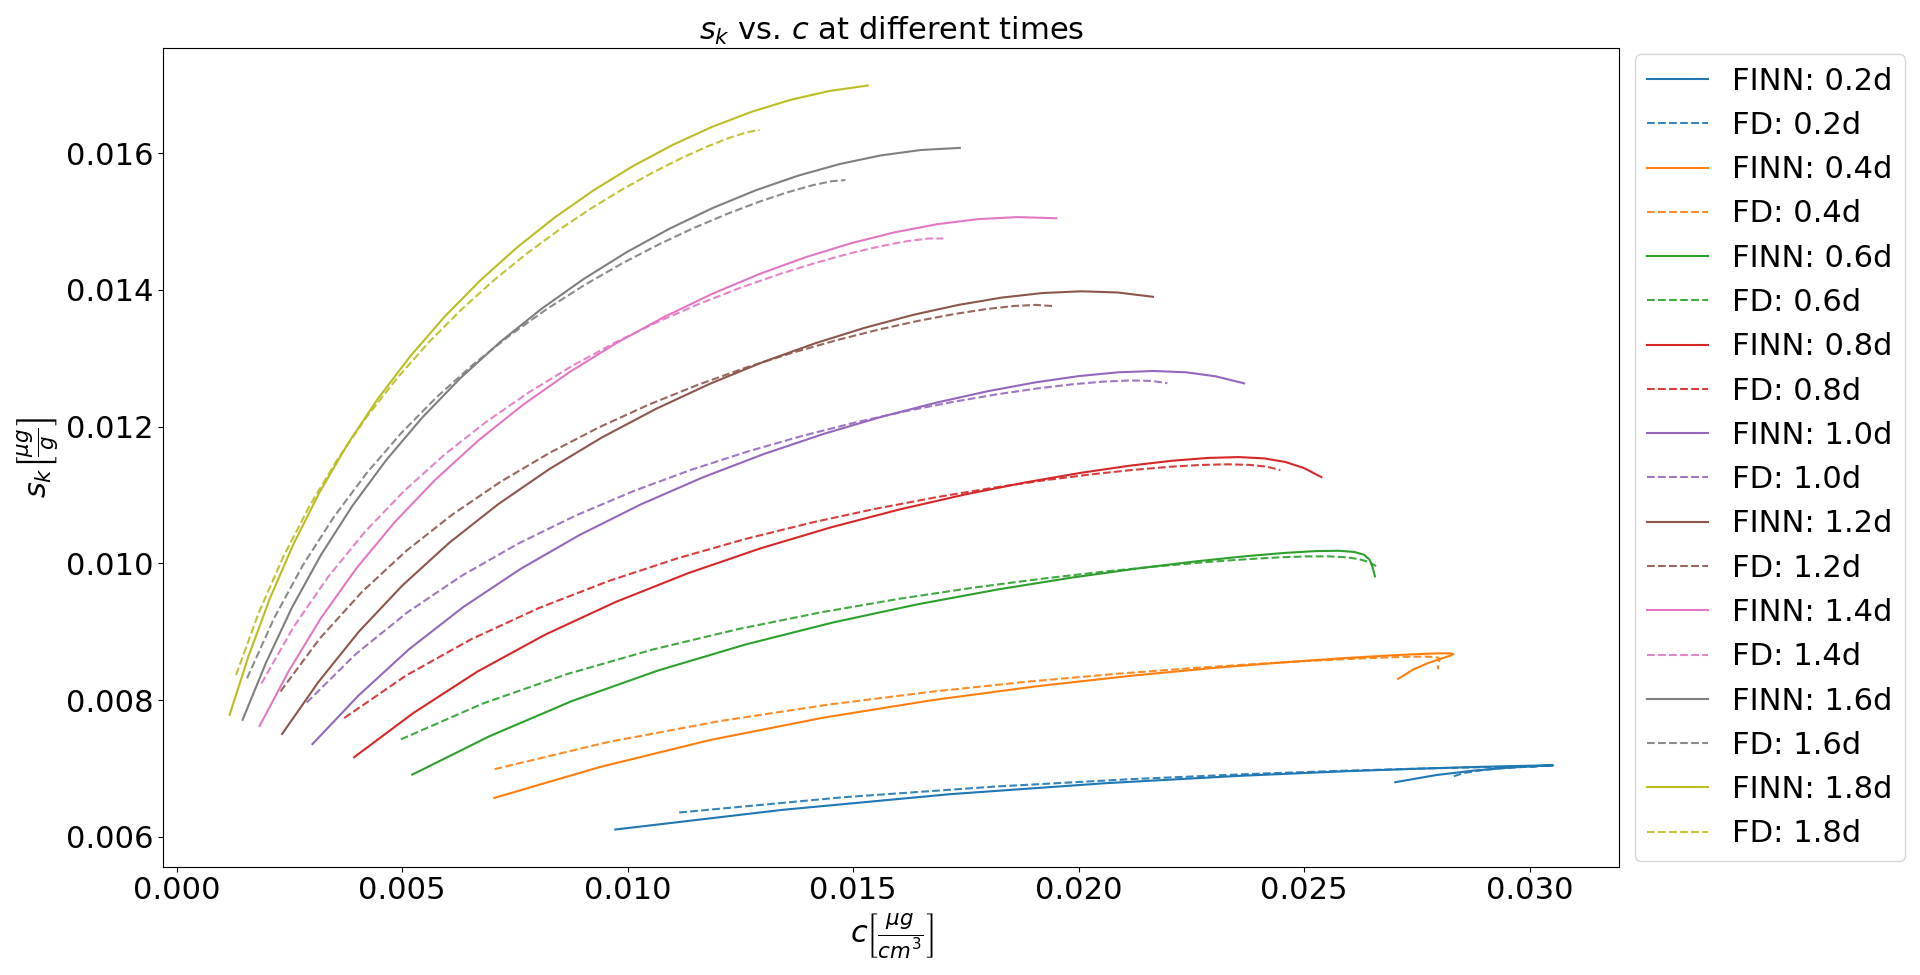
\includegraphics[width=\textwidth]{images/res_sorp_synt_FGR_500.png}
\caption[Comparison of FD and FINN sorption behavior, run e]{Comparison of FD and FINN solution: The unknowns $s_k$ and $c$ plotted at fixed time steps, run e.}
\label{fig:res_sorp_synt_FGR_500}
\end{figure}\\
The model has difficulties at regions near the outflow and thus also in approximating the BTC (Fig. \ref{fig:res_diff_synt_FGR_500_m}, left and Fig. \ref{fig:res_btc_synt_FGR_500_m}, left). Using only the BTC data for loss calculation could improve this issue, which is done in the next steps for experimental data.\\
Interestingly we received for run d (Fig. \ref{fig:res_diff_synt_F_m}, right)
\begin{equation}
    |s_{k,FD} - s_{k, FINN}| \leq 0.0015 \qquad \forall (x, t) \in \Omega_x \times \Omega_t,
\end{equation}
and for run e (Fig. \ref{fig:res_diff_synt_FGR_500_m}, right)
\begin{equation}
    |s_{k,FD} - s_{k, FINN}| \leq 0.0008 \qquad \forall (x, t) \in \Omega_x \times \Omega_t.
\end{equation}
The absolute difference of $s_{k,FD}$ and $s_{k, FINN}$ is, compared to the model of run d smaller. The high loss value is mainly due to difficulties of the model in regions close to the outflow. Within the contaminated soil layer the model approximates the FD solution very well and better than in run d. Thus the $c$ - $s_k$ sorption isotherms are learned with higher accuracy in run e (Fig. \ref{fig:res_sorp_synt_FGR_500}).\\
\\
There was also performed a run that learns functional relations with only 300 training epochs. Corresponding results are available in the appendix (Figs. \ref{fig:res_ov_synt_FGR_300_m}, \ref{fig:res_diff_synt_FGR_300_m}, \ref{fig:res_btc_synt_FGR_300_m}, \ref{fig:res_sorp_synt_FGR_300}). Interestingly, at constant epoch numbers and learning rates, FINN seemed to perform better when all 3 functional relations $F$, $G$, and $R$ and not only $F$ were learned.
\FloatBarrier
\section{Learning from Experimental Data}
Performing loss calculation with data of experiment N1\_1 or N1\_3 of Bierbaum et al. also enabled training and testing of FINN models. In contrast to the experiment, the Darcy flux was assumed to be constant and averaged over the entire simulation time. Used material parameters for experiment N1\_1 are described in Table \ref{table:meta_run_exp} and discretization parameters in Table \ref{tab:disc_run_exp}.
\begin{table}[h!]
    \centering
    \begin{tabular}{h|ccccccc}
     \quad & $n_{e} \left[-\right]$ & $\rho \left[\frac{g}{cm^3}\right]$ & $D_e \left[\frac{cm^2}{d}\right]$ & $\alpha_l \left[cm\right]$ & $c_{init} \left[\frac{\mu g}{cm^3}\right]$ & $s_{k, init} \left[\frac{\mu g}{g}\right]$ & $q \left[\frac{cm}{d}\right]$  \\ [0.2 cm] \hline
     sand & 0.31 & NaN & 0 & 5 & 0 & 0 & 31.68 \\
     soil & 0.4 & 1.58 & 2.5 & 9 & 0.032 & 0.0053 & 31.68 \\
    \end{tabular}
    \caption{Material parameters of N1\_1 for FINN.}
    \label{table:meta_run_exp}
\end{table}
\begin{table}[h!]
    \centering
    \begin{tabular}{cccccc}
      $T_{MAX} \left[d\right]$ & $T_{STEPS} \left[-\right]$ & $X_{LENGTH} \left[cm\right]$ & $X_{STEPS} \left[-\right]$ & top & bot \\ [0.2 cm] \hline
      141.76 & 38000 & 55 & 28 & 4 & 24
    \end{tabular}
    \caption{Discretization parameters for FINN.}
    \label{tab:disc_run_exp}
\end{table}

\subsection{Learning Parameters}
In order to reproduce work of Bierbaum et al. with FINN, the parameter $f$ as ratio between kinetically sorbed and instantaneously sorbed concentration was investigated. The remaining non-learnable model parameters are given in Table \ref{table:model_run_f}.
\begin{table}[h!]
    \centering
    \begin{tabular}{h|cccc}
         \quad & $k_d \left[\frac{cm^3}{d}\right]$ & $\beta \left[-\right]$ & $\alpha_k \left[\frac{1}{d}\right]$ \\ [0.2 cm] \hline
         soil & 4.5 & 0.98 & 0.005
    \end{tabular}
    \caption{Model parameters for FINN, run f.}
    \label{table:model_run_f}
\end{table}
\FloatBarrier
\\
\\
\textbf{Run f - Learn $f$}\\
As initial guess the optimized $f_{init}$ of Bierbaum et al. was used. Using the $L_{I}$ loss function, an optimal $\hat{f}$ was assumed after 99 of 100 epochs (Tab. \ref{table:learn_exp_f}, Figs \ref{fig:res_ov_exp_pf}, \ref{fig:res_loss_exp_pf}). However, the values found for f were very similar.
\begin{table}[h!]
    \centering
    \begin{tabular}{c|cccc}
         run f& value &epochs& lr& $L_{I}$ \\[0.2 cm] \hline
         $f_{init}[-]$ & 0.93 & / & /& $2.64 \times 10^{-1}$ \\
         $\hat{f}[-]$ & 0.9161 & 100 & 0.1 & $2.63 \times 10^{-1}$\\
    \end{tabular}
    \caption[Learning $f$ using experimental data, run f]{Comparison of optimal $f$ of Bierbaum et al. ($f_{init}$) with FINN predicted ($\hat{f}$). $L_{I}$ is the loss for $f_{init}$ and $\hat{f}$ respectively, run f.}
    \label{table:learn_exp_f}
\end{table}
\begin{figure}[h!]
	\centering
	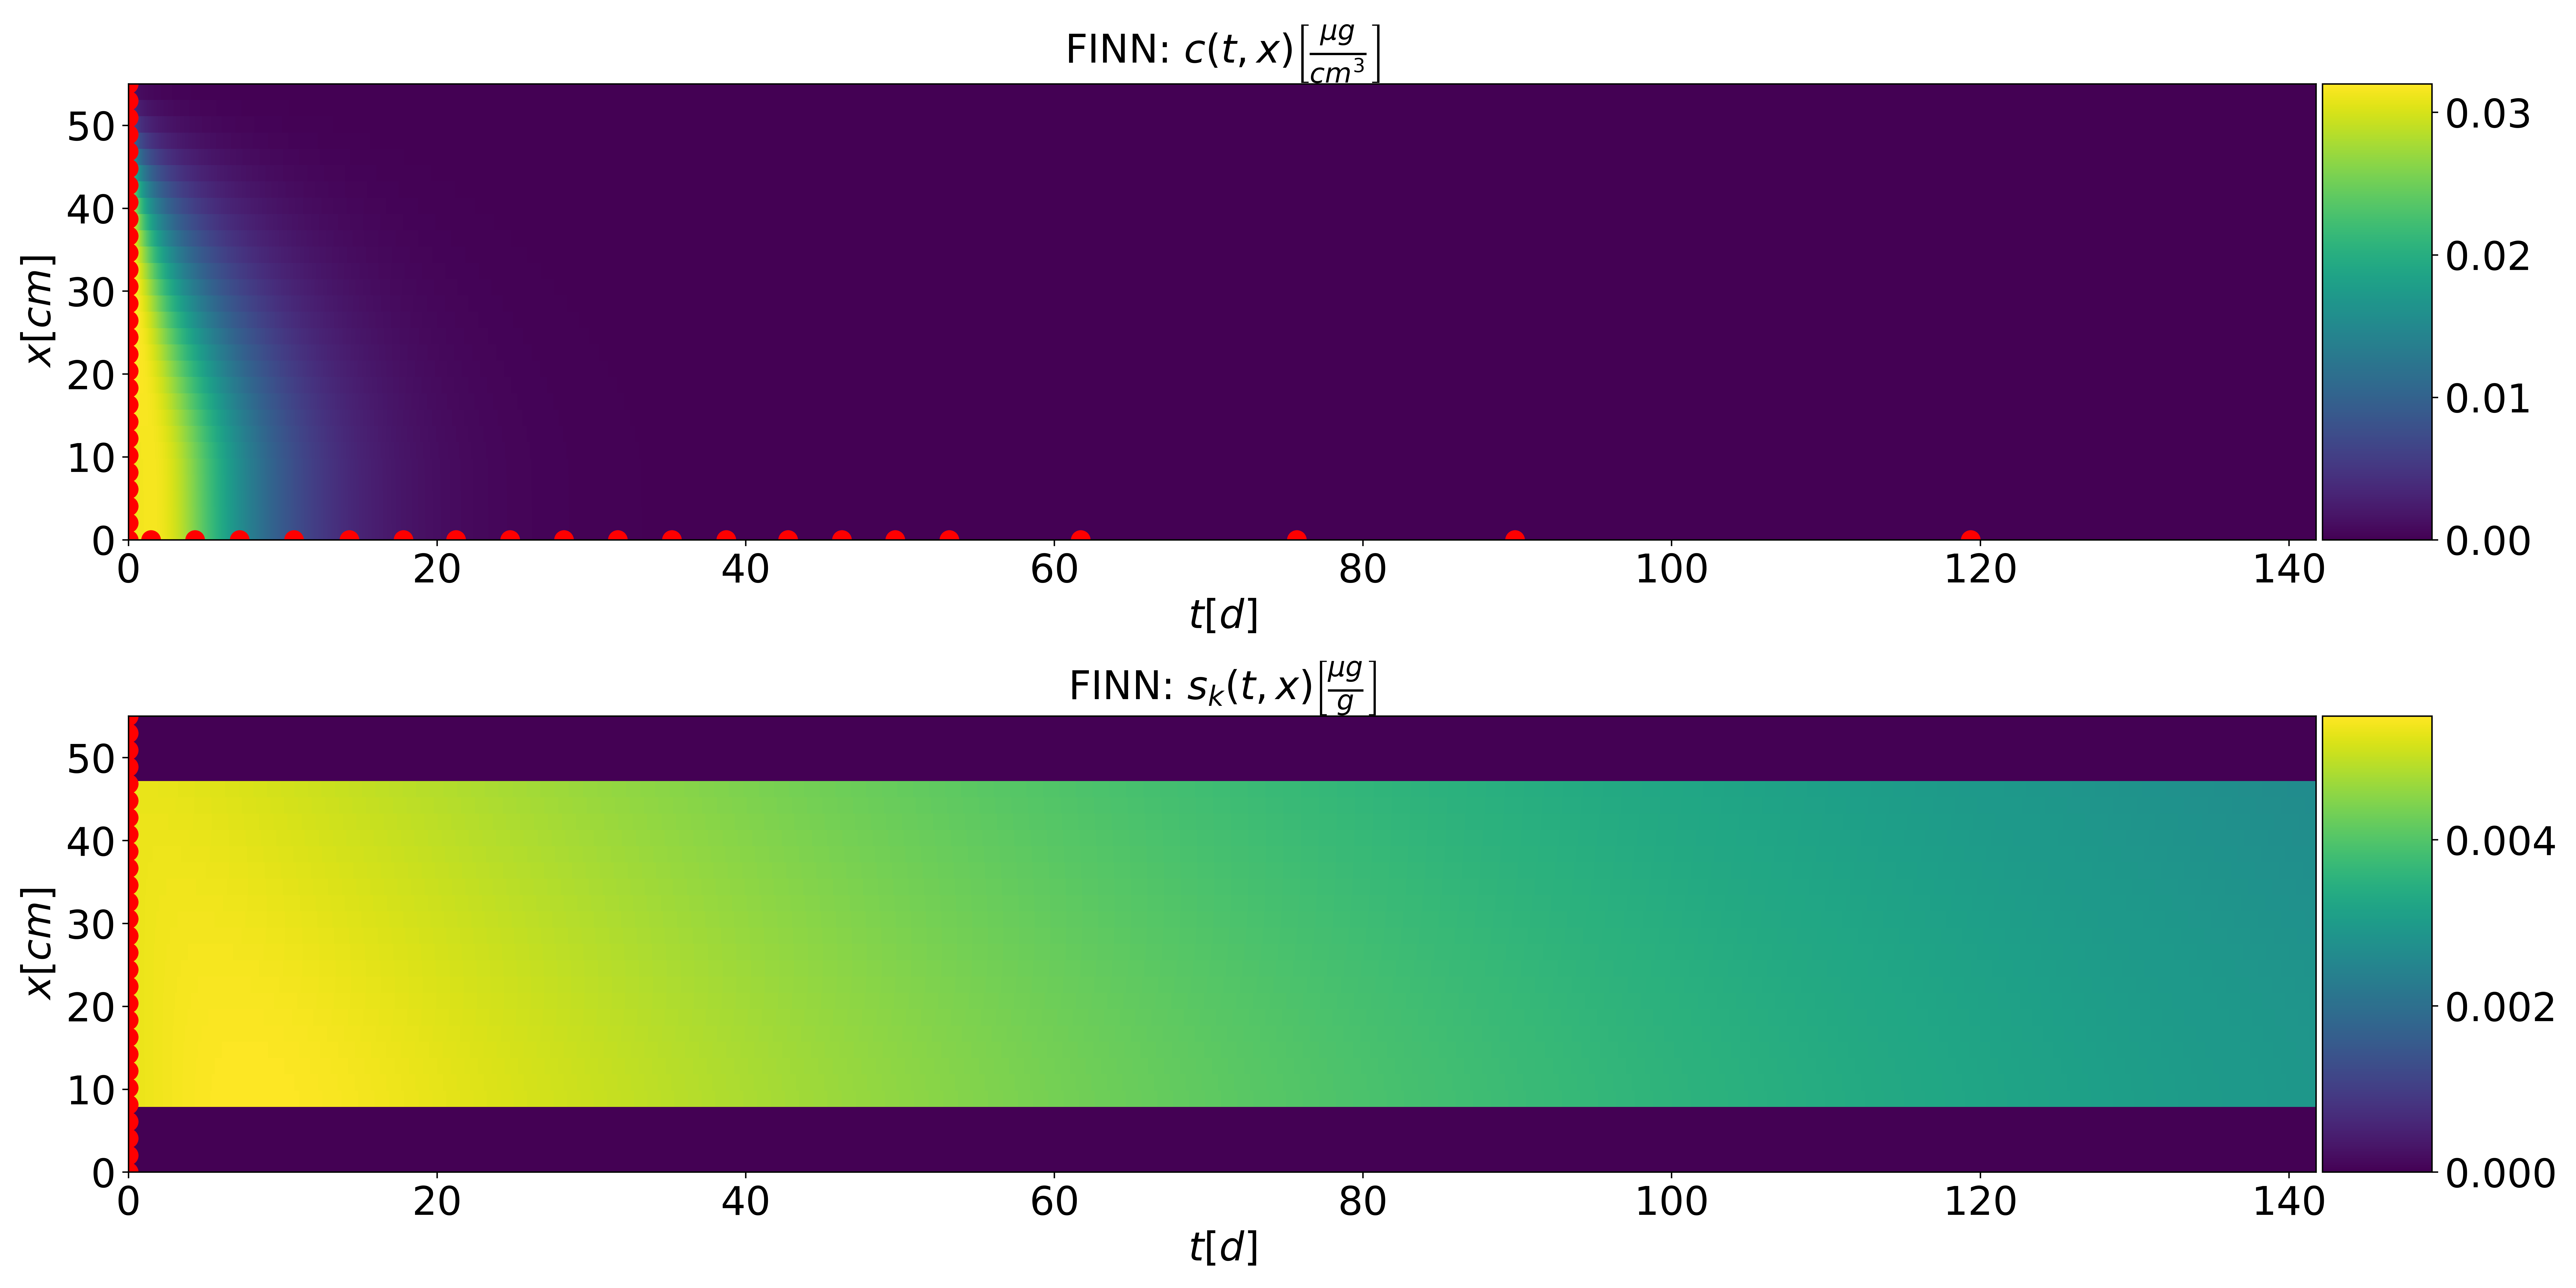
\includegraphics[scale=0.29]{images/res_ov_exp_pf.png}
\caption[FINN predicted solution after training, run f]{FINN prediction of $c$ (top) and $s_k$ (bottom) after training. Red points describe initial conditions and BTC concentrations of experiment N1\_1 data, which were used for the loss calculation, run f.}
\label{fig:res_ov_exp_pf}
\end{figure}
\begin{figure}[h!]
	\centering
	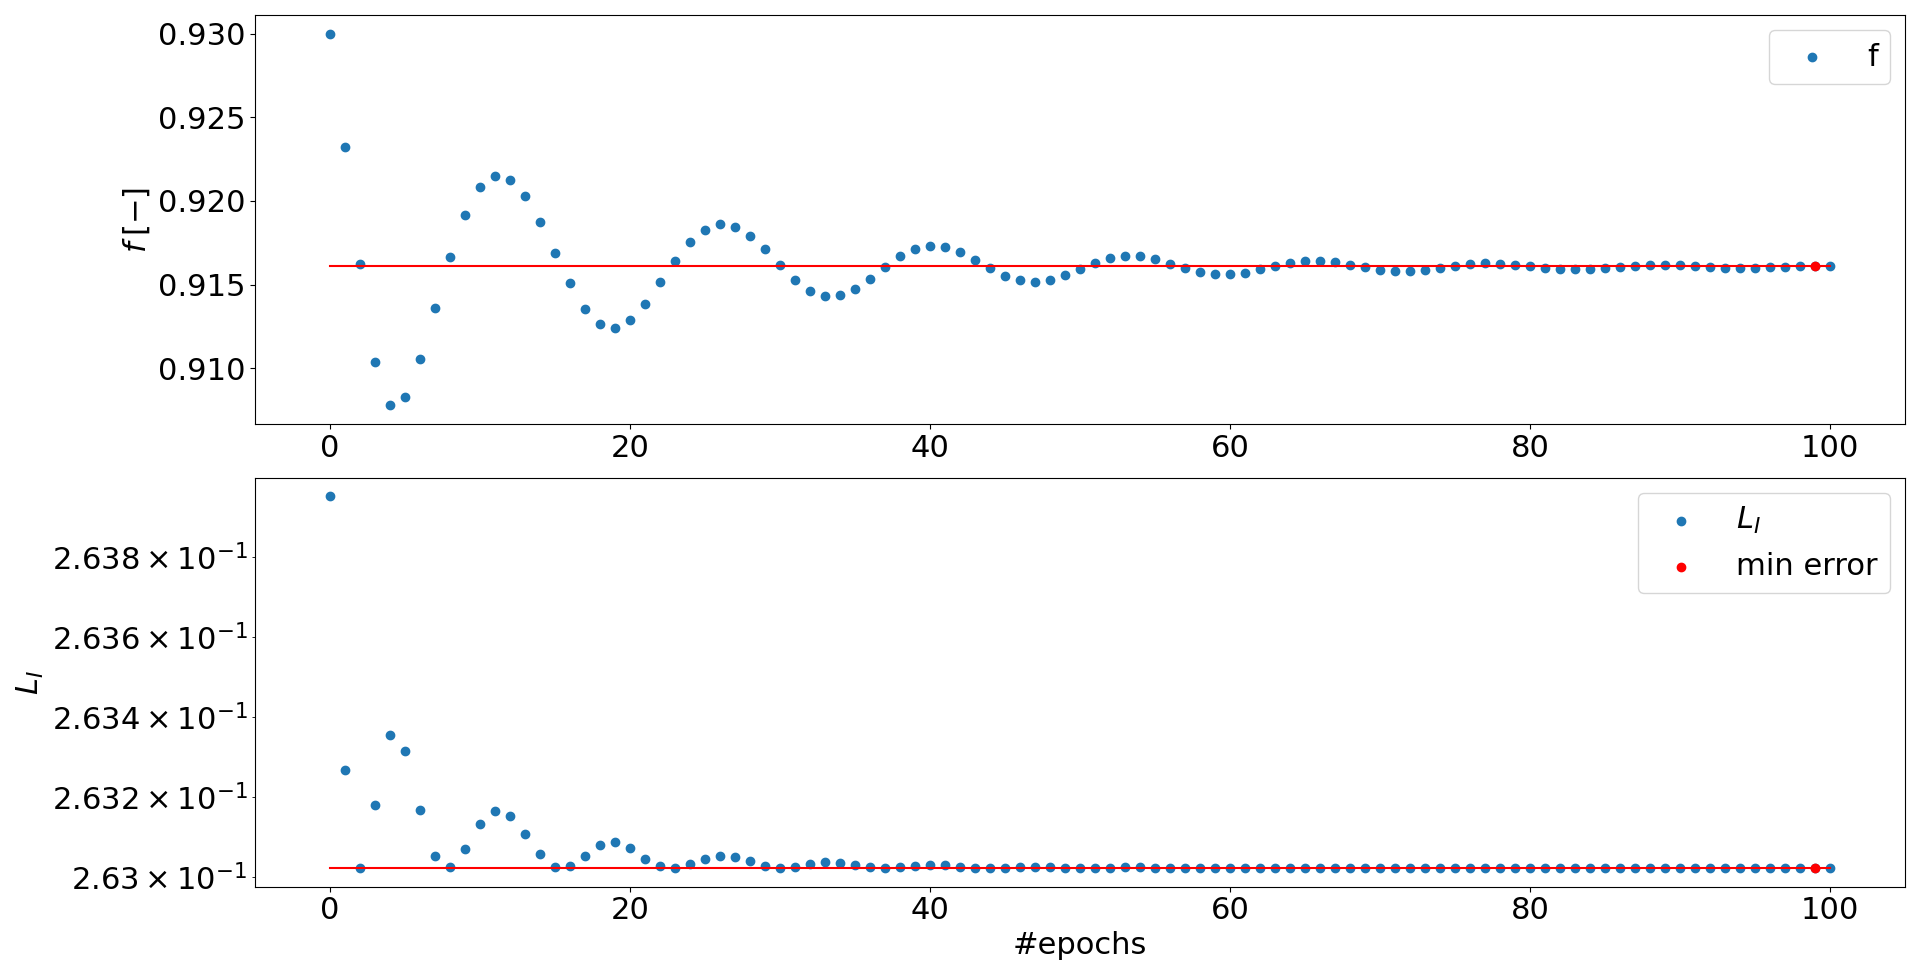
\includegraphics[scale=0.29]{images/res_loss_exp_pf.png}
\caption[Loss, run f]{Course of predicted $\hat{f}$ (top) with corresponding $L_{I}$ loss (bottom). Optimal $\hat{f}$ and minimal loss value are colored in red, run f.}
\label{fig:res_loss_exp_pf}
\end{figure}\\
\\
In addition to BTC data, experimental data also contained the course of the totally sorbed concentration $s$, which is the sum of $s_k$ and $s_e$ at the end of the experiment, which was approximately homogeneously distributed. The $\hat{f}$ found by FINN approximated this course worse than $f_{init}$ (Fig. \ref{fig:res_btc_exp_pf_comp}, right).
\begin{figure}[h!]
	\centering
	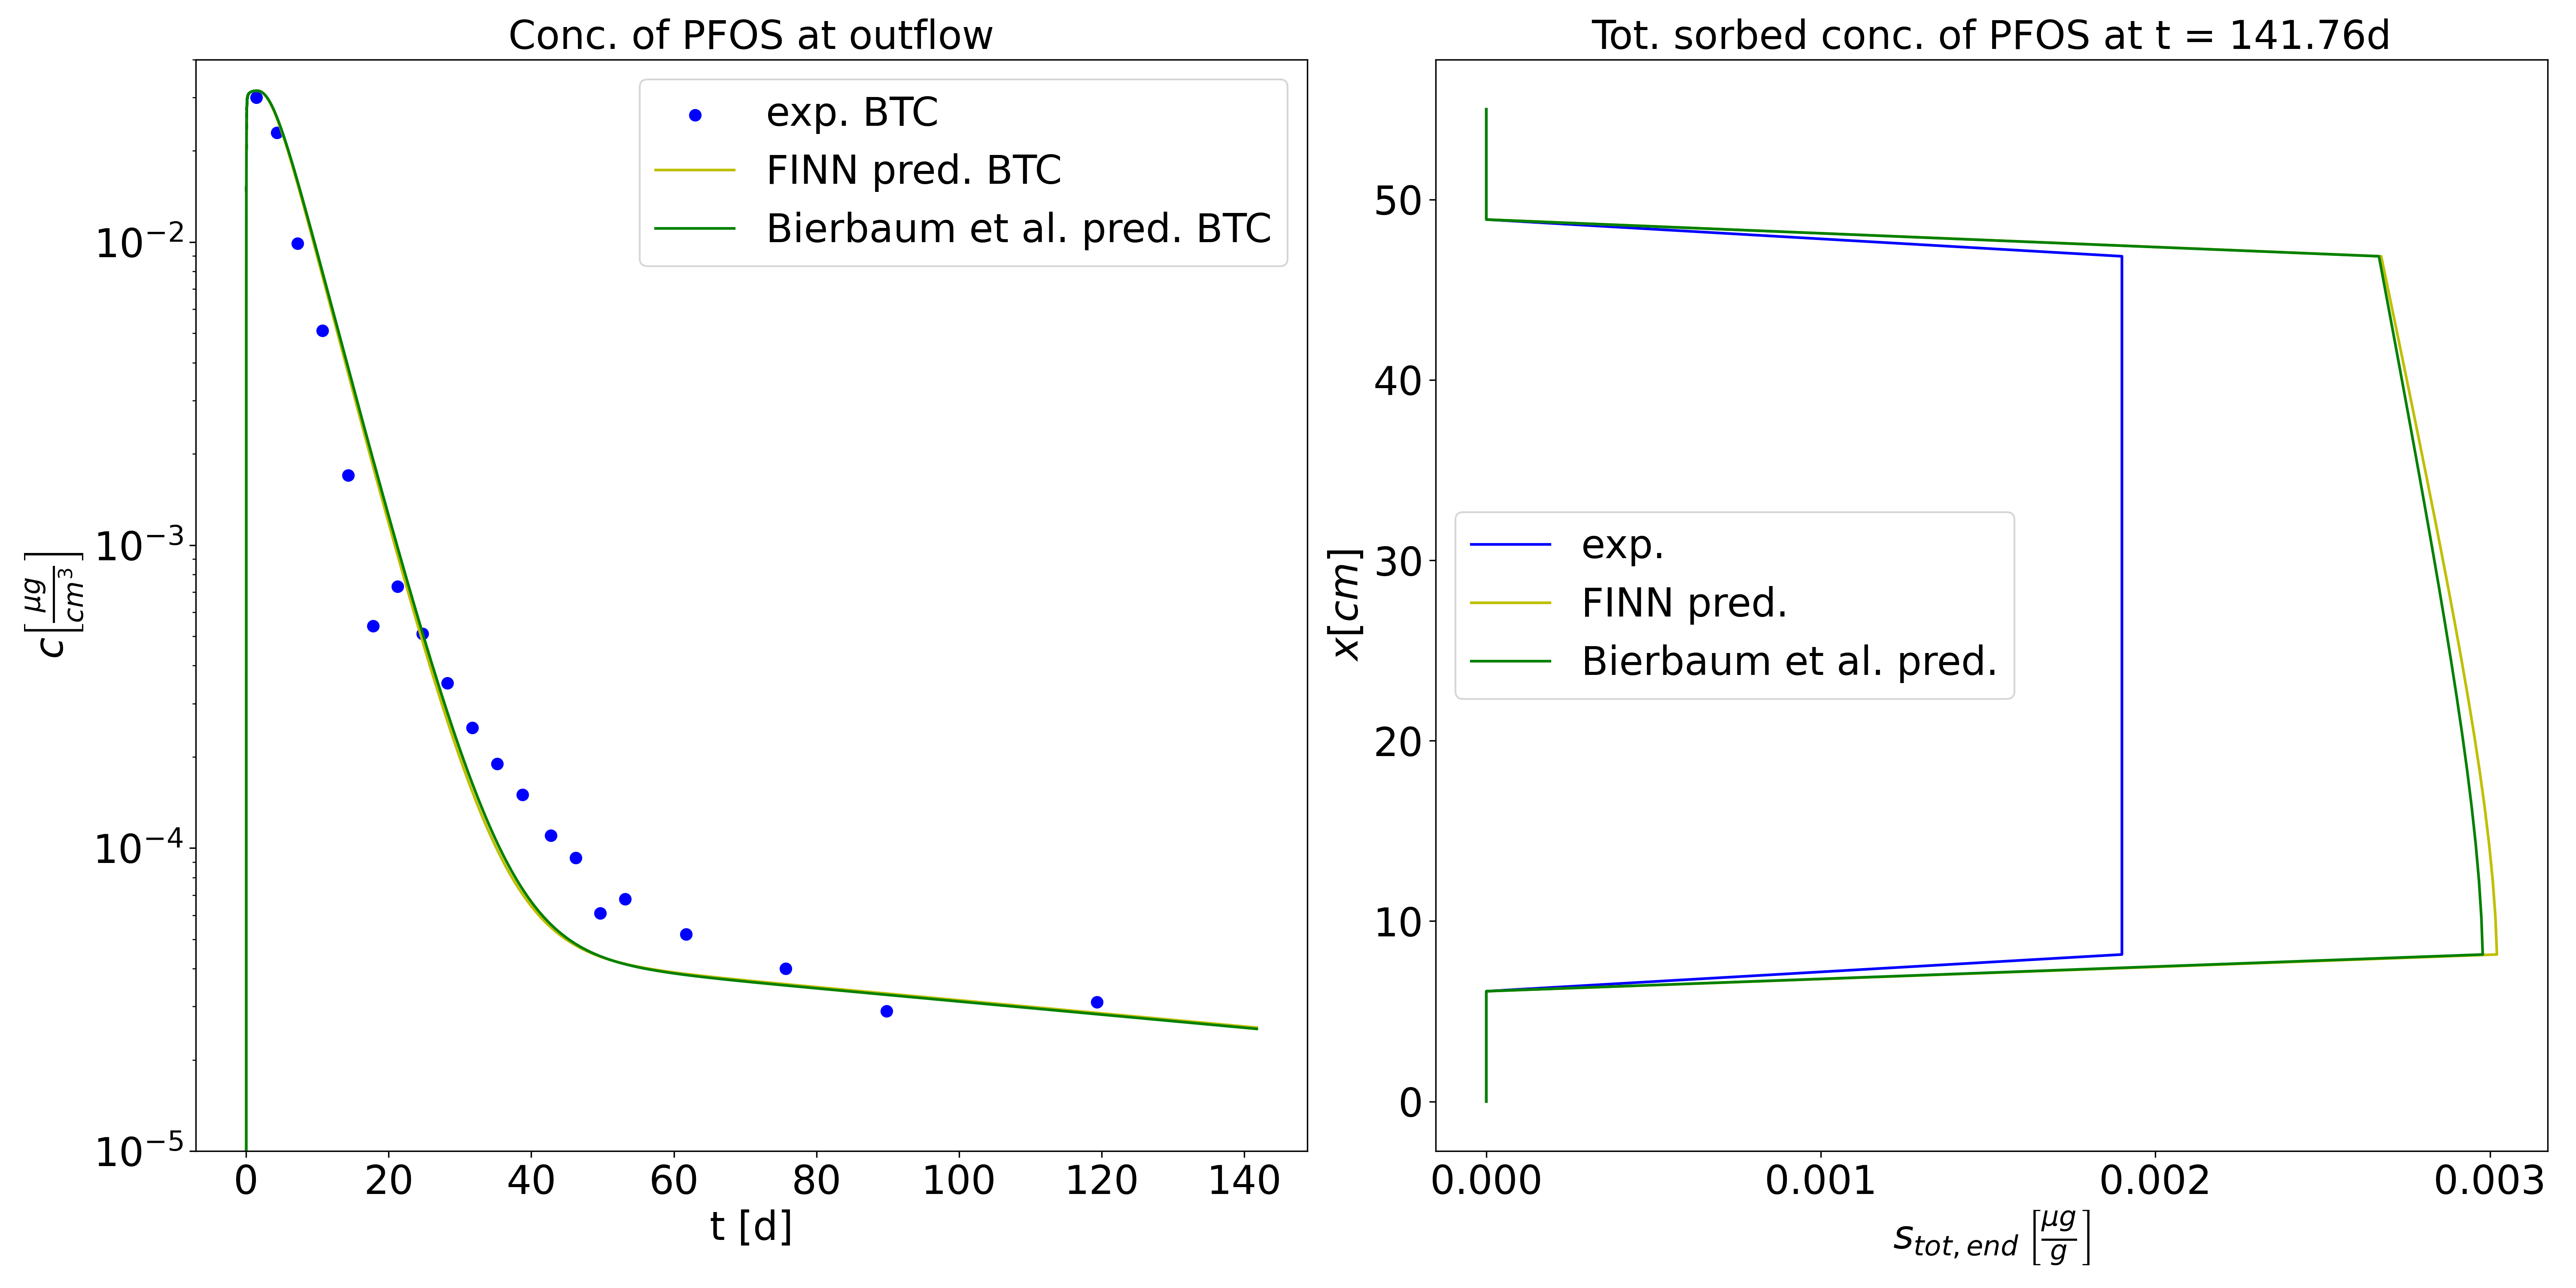
\includegraphics[scale=0.29]{images/res_btc_exp_pf_comp.png}
\caption[FINN predicted BTC, run f]{Optimizing $f$ using experimental BTC (left). Comparison of FINN predicted parameter $\hat{f}$ and $f_{init}$ with respect to experimental total sorbed concentration at the end of the experiment (right), run f.}
\label{fig:res_btc_exp_pf_comp}
\end{figure}
Since $\hat{f}$ of FINN is smaller than the $f_{init}$ of Bierbaum et al., the share of kinetically sorbed PFOS is higher ($f=0$ corresponds to complete kinetic sorption), which is observable in the $s_k$ - $c$ sorption isotherm too (Fig. \ref{fig:res_sorp_exp_pf}).
\begin{figure}[h!]
	\centering
	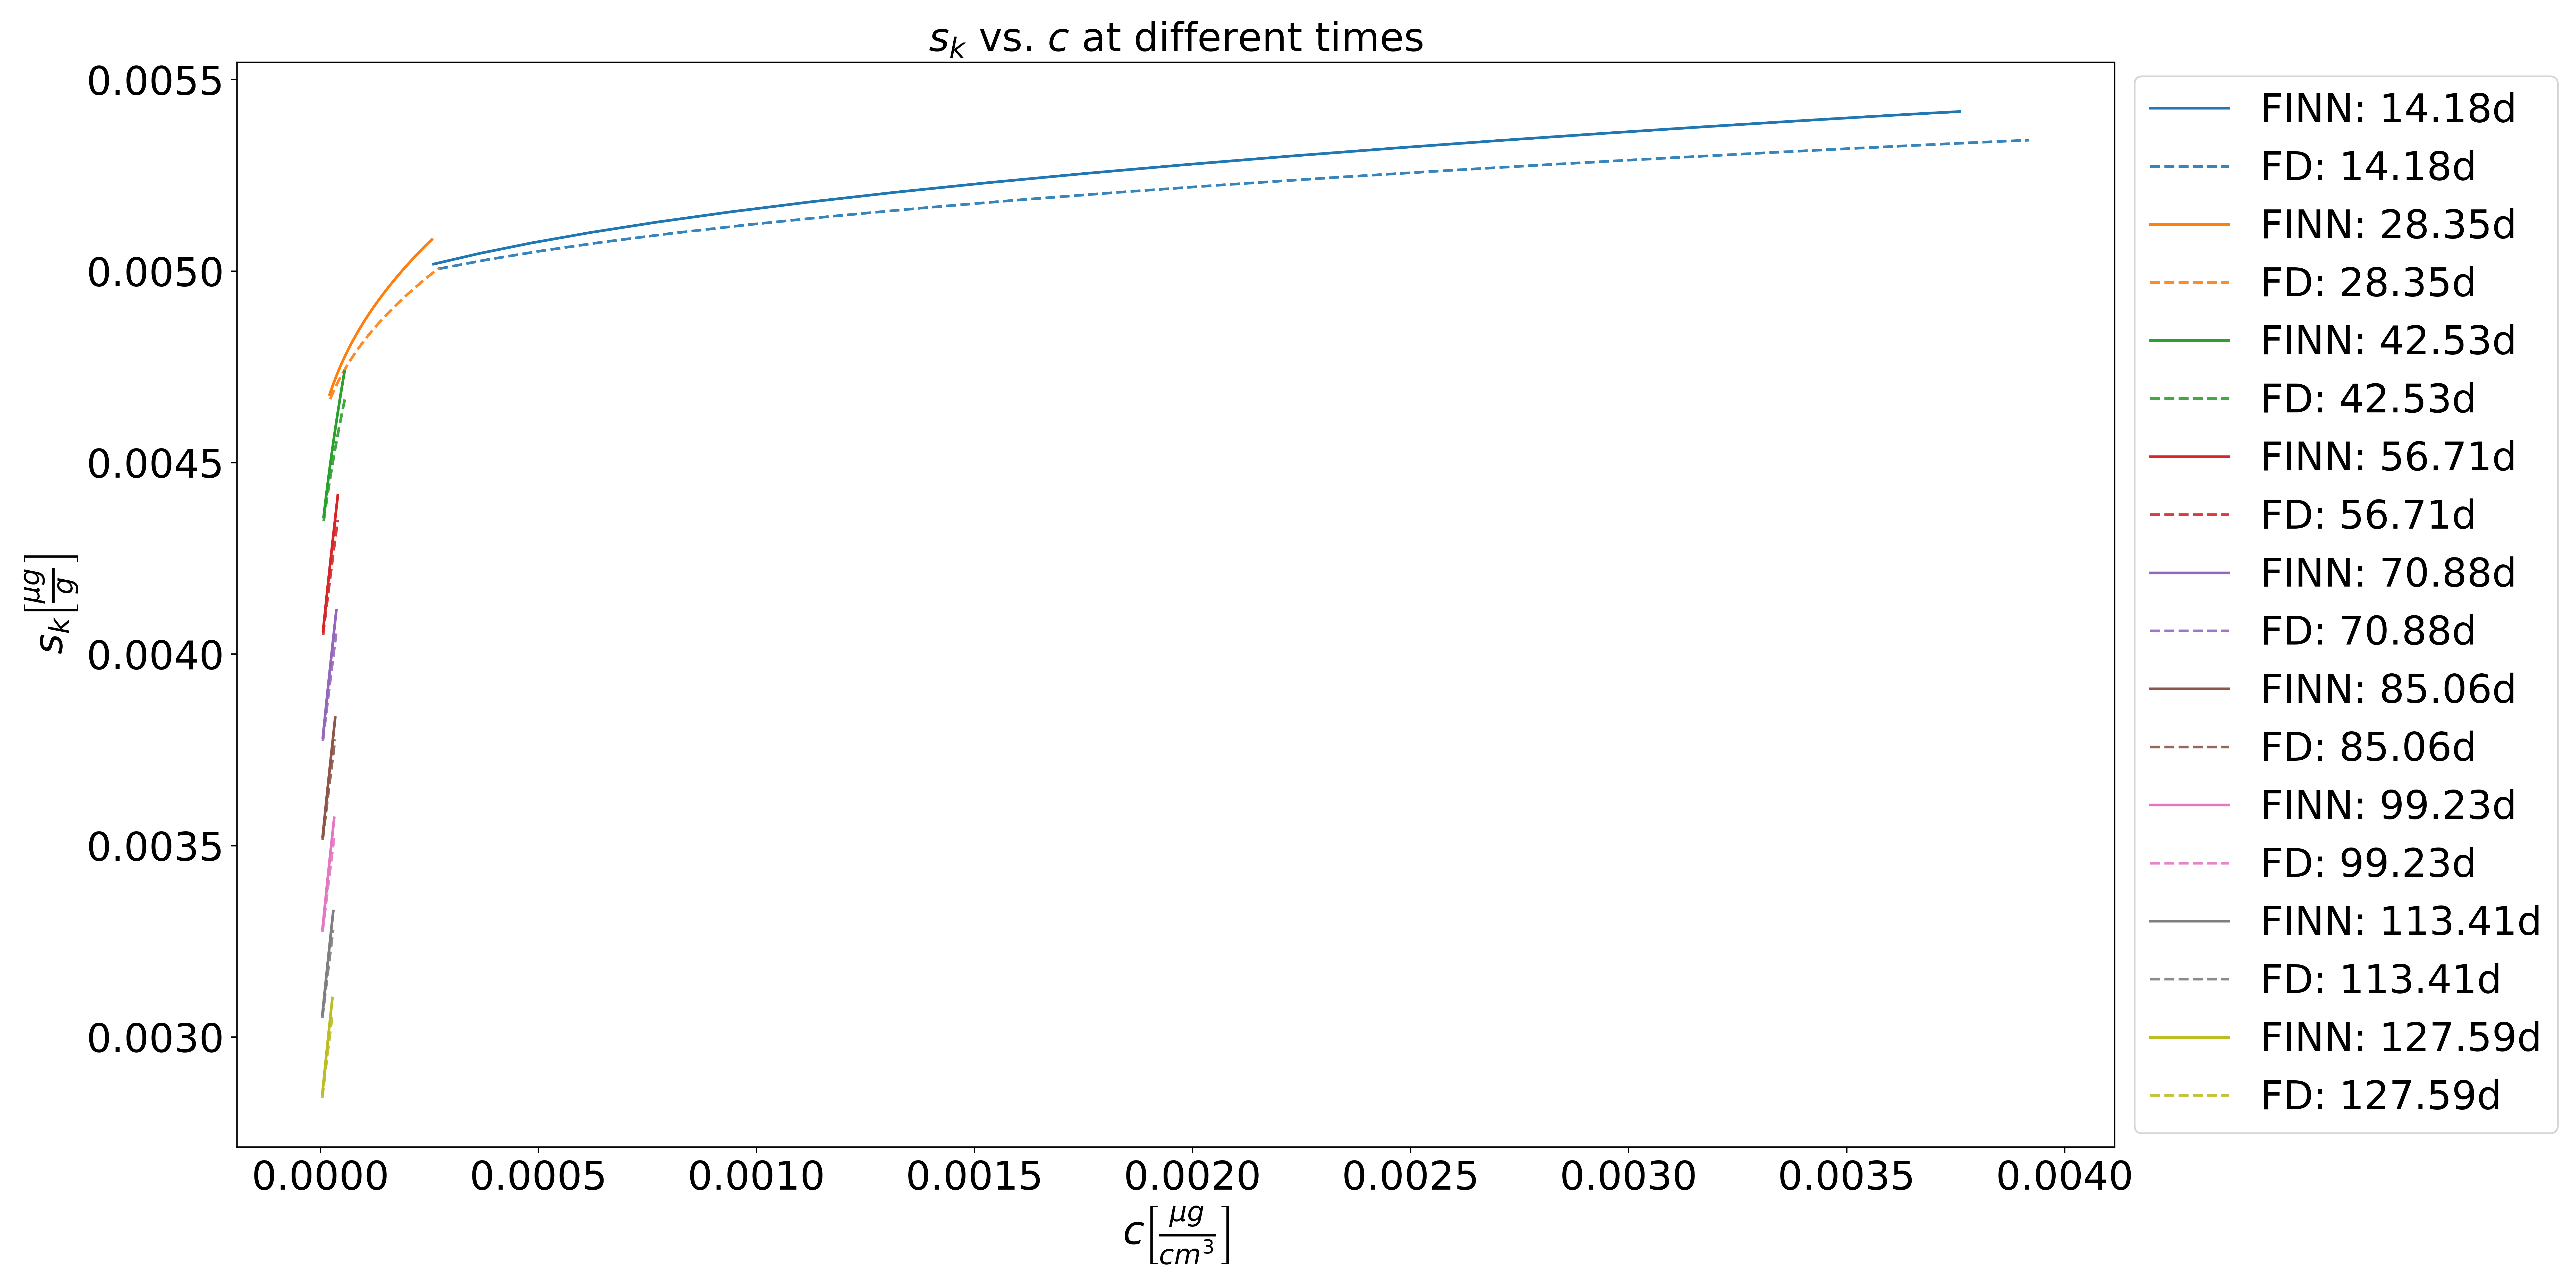
\includegraphics[scale=0.29]{images/res_sorp_exp_pf.png}
\caption[FINN predicted sorption behavior, run f]{Comparison of FD solution with given $f_{init}$ from Bierbaum et al. and FINN solution: The unknowns $s_k$ and $c$ plotted at fixed time steps, run f.}
\label{fig:res_sorp_exp_pf}
\end{figure}
\FloatBarrier
\subsection{Learning Functional Relations}
\textbf{Run g - Learn Time-dependent $F$, $G$ and $R$}\\
Each function $F$, $G$ and $R$, thus the entire sorption behavior of PFOS in experiment was approximated by a 2-100-1000-100-1 time-dependent DNN with biases and scaling term (Tab. \ref{tab:FGR_exp}, Fig. \ref{fig:res_ov_exp_FGR}). Thus each function consists of
\begin{equation}
   \#\theta = \underbrace{2 \cdot 100 + 100 \cdot 1000 + 1000 \cdot 100 + 100 \cdot 1}_{weights} + \underbrace{100 + 1000 + 100 + 1}_{biases} + \underbrace{1}_{scale} = 201502
\end{equation}
parameters. The number of parameters of the DNN for experimental data approximation was chosen larger than for synthetic data, since more time steps have to be done, which increases the number of input samples $(t, c)$ or $(t, s_k)$ respectively. Smaller architectures of DNNs could lead to data underfitting.
\begin{table}[h!]
    \centering
    \begin{tabular}{c|c||cccc}
    train & init & \multicolumn{4}{c}{Learning schedule}\\
    learn & scalings & epochs & lr & $L_{II}$ & $L_{III}$ \\[0.2 cm] \hline
          $F$ & $f_{sc} = 0.1$ & 300 & 0.001 & $2.32\times 10^{-1}$ & $ 0.00 $\\
          $G$ & $g_{sc} = 0.0001$ & & & &\\
          $R$ & $r_{sc} = 1$ & & & & 
        \end{tabular}
    \caption[FINN training with unknown time-dependent functions $F$, $G$, $R$, run g]{FINN training with unknown time-dependent functions $F$, $G$, $R$, run g.}
    \label{tab:FGR_exp}
\end{table}
\begin{figure}[h!]
	\centering
	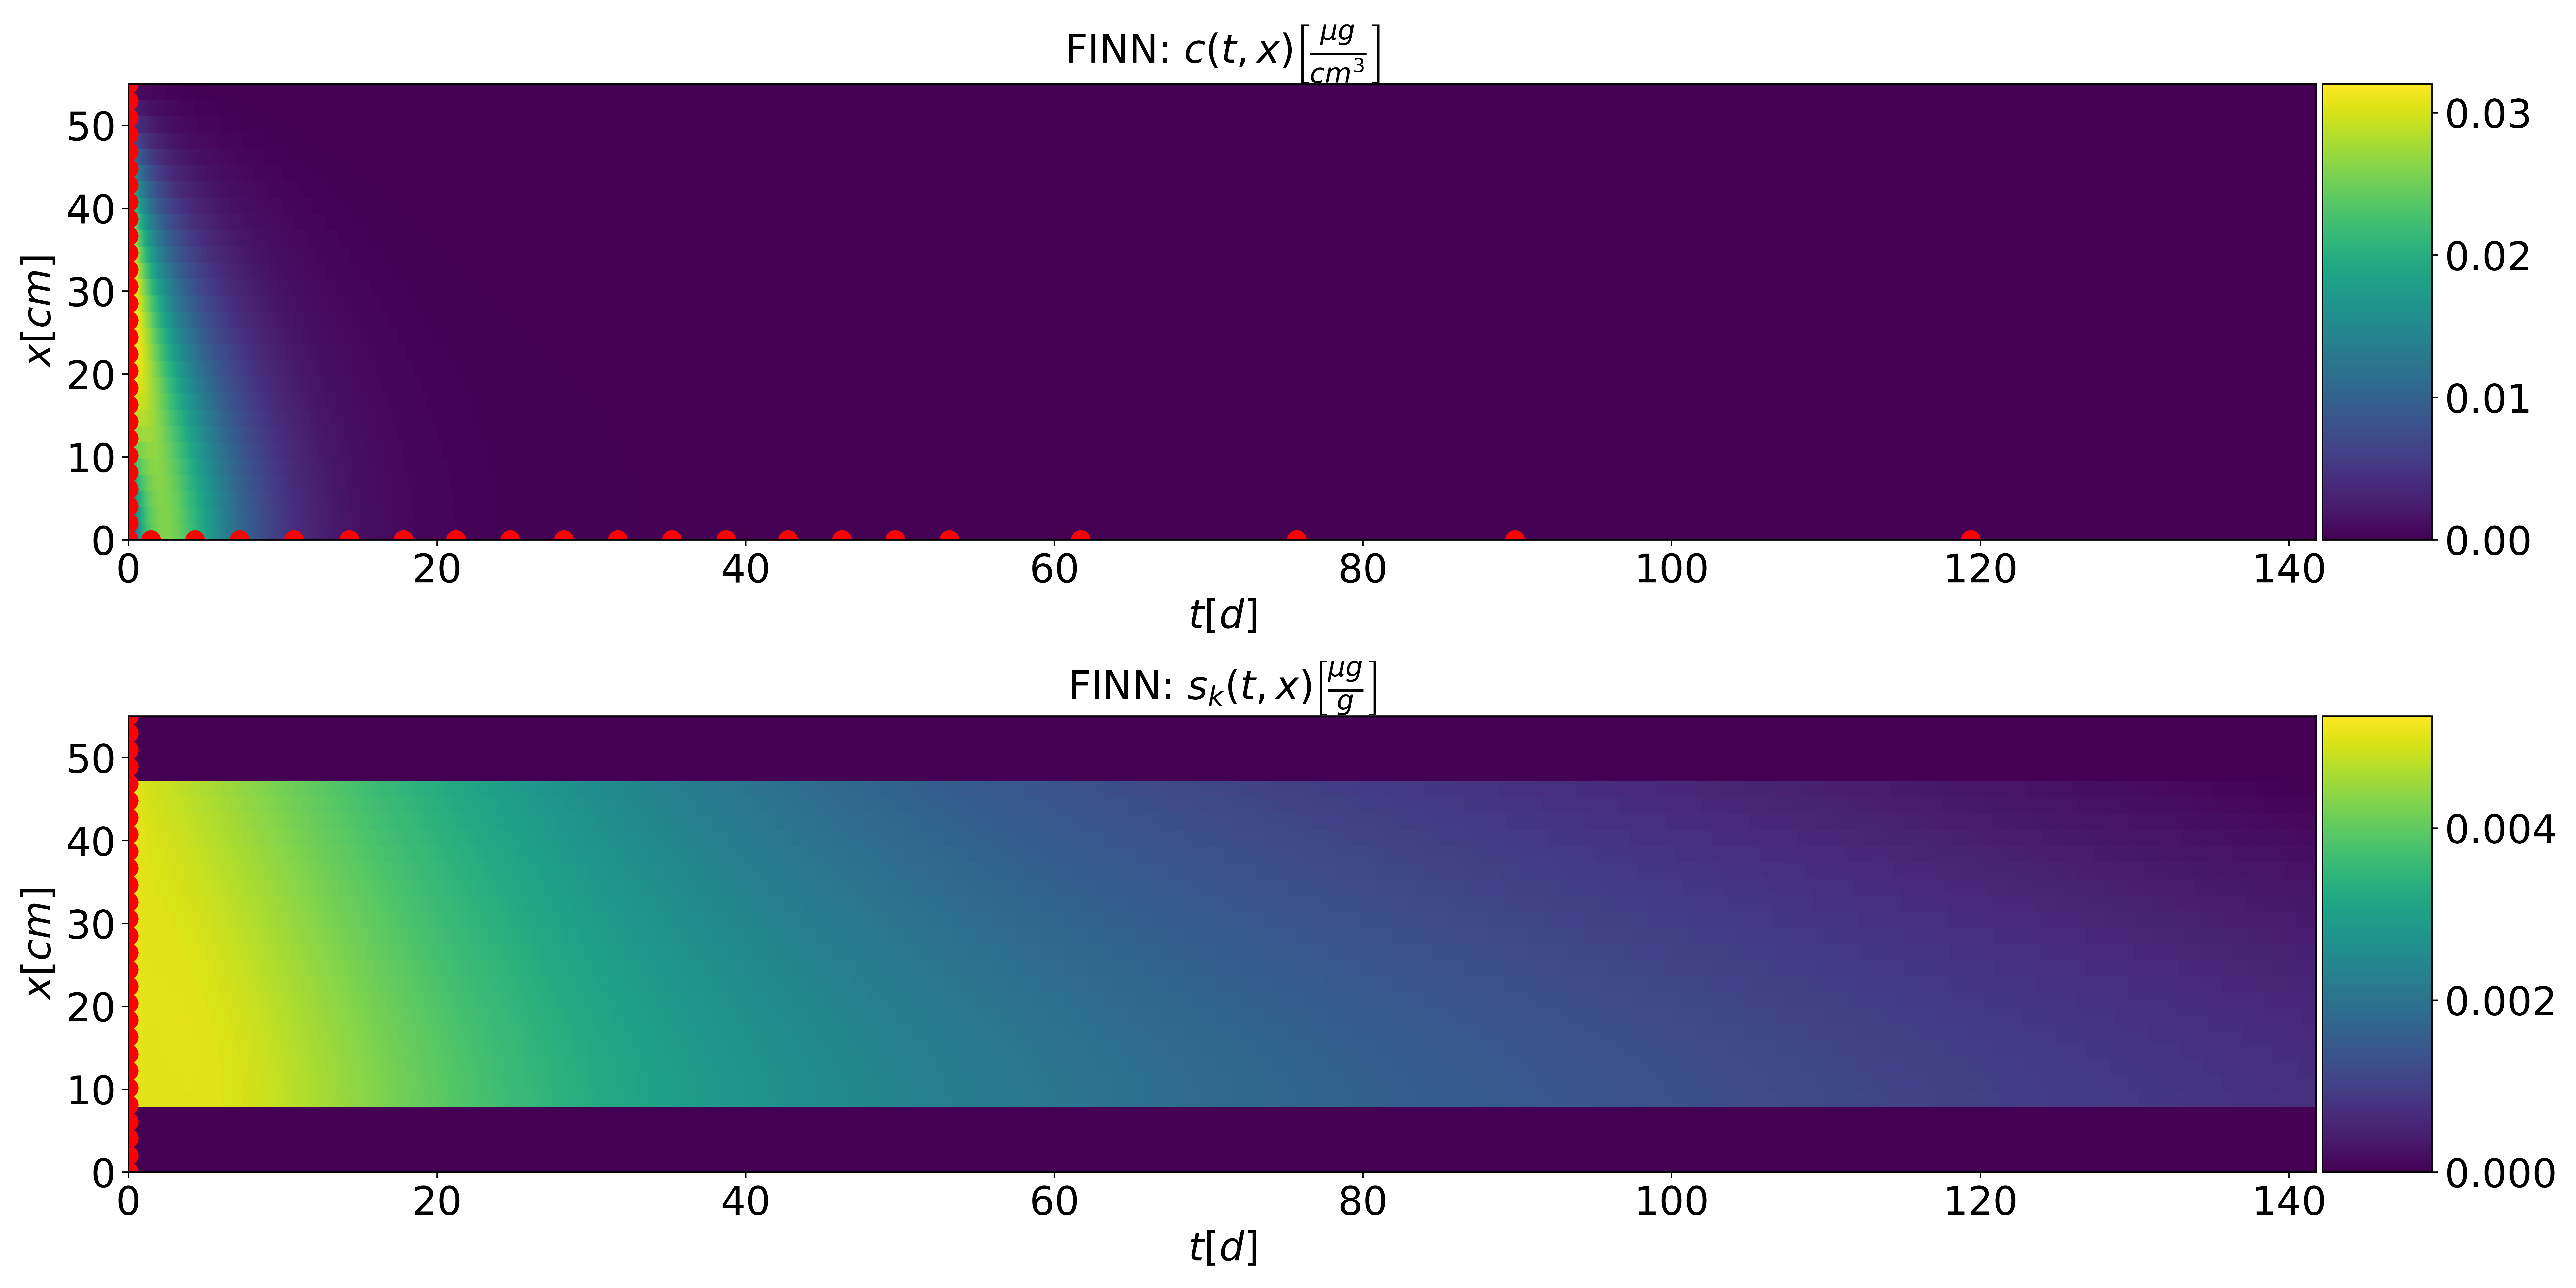
\includegraphics[width=\textwidth]{images/res_ov_exp_FGR.png}
\caption[FINN predicted solution after training, run g]{FINN prediction of $c$ (top) and $s_k$ (bottom) after training.  Red points describe initial conditions and BTC concentrations of experiment N1\_1 data, which were used for the loss calculation, run g.}
\label{fig:res_ov_exp_FGR}
\end{figure}\\
Under the condition that predicted concentrations have to take positive values, the calculated combined loss value during training was lowest after 116 of 300 training epochs. For larger numbers of epochs, the scaling factor introduced as a punishment for negative learned concentration values described in eq. \ref{eq:LOSS_pen} was too small (Fig. \ref{fig:res_loss_exp_FGR}).
\begin{figure}[h!]
	\centering
	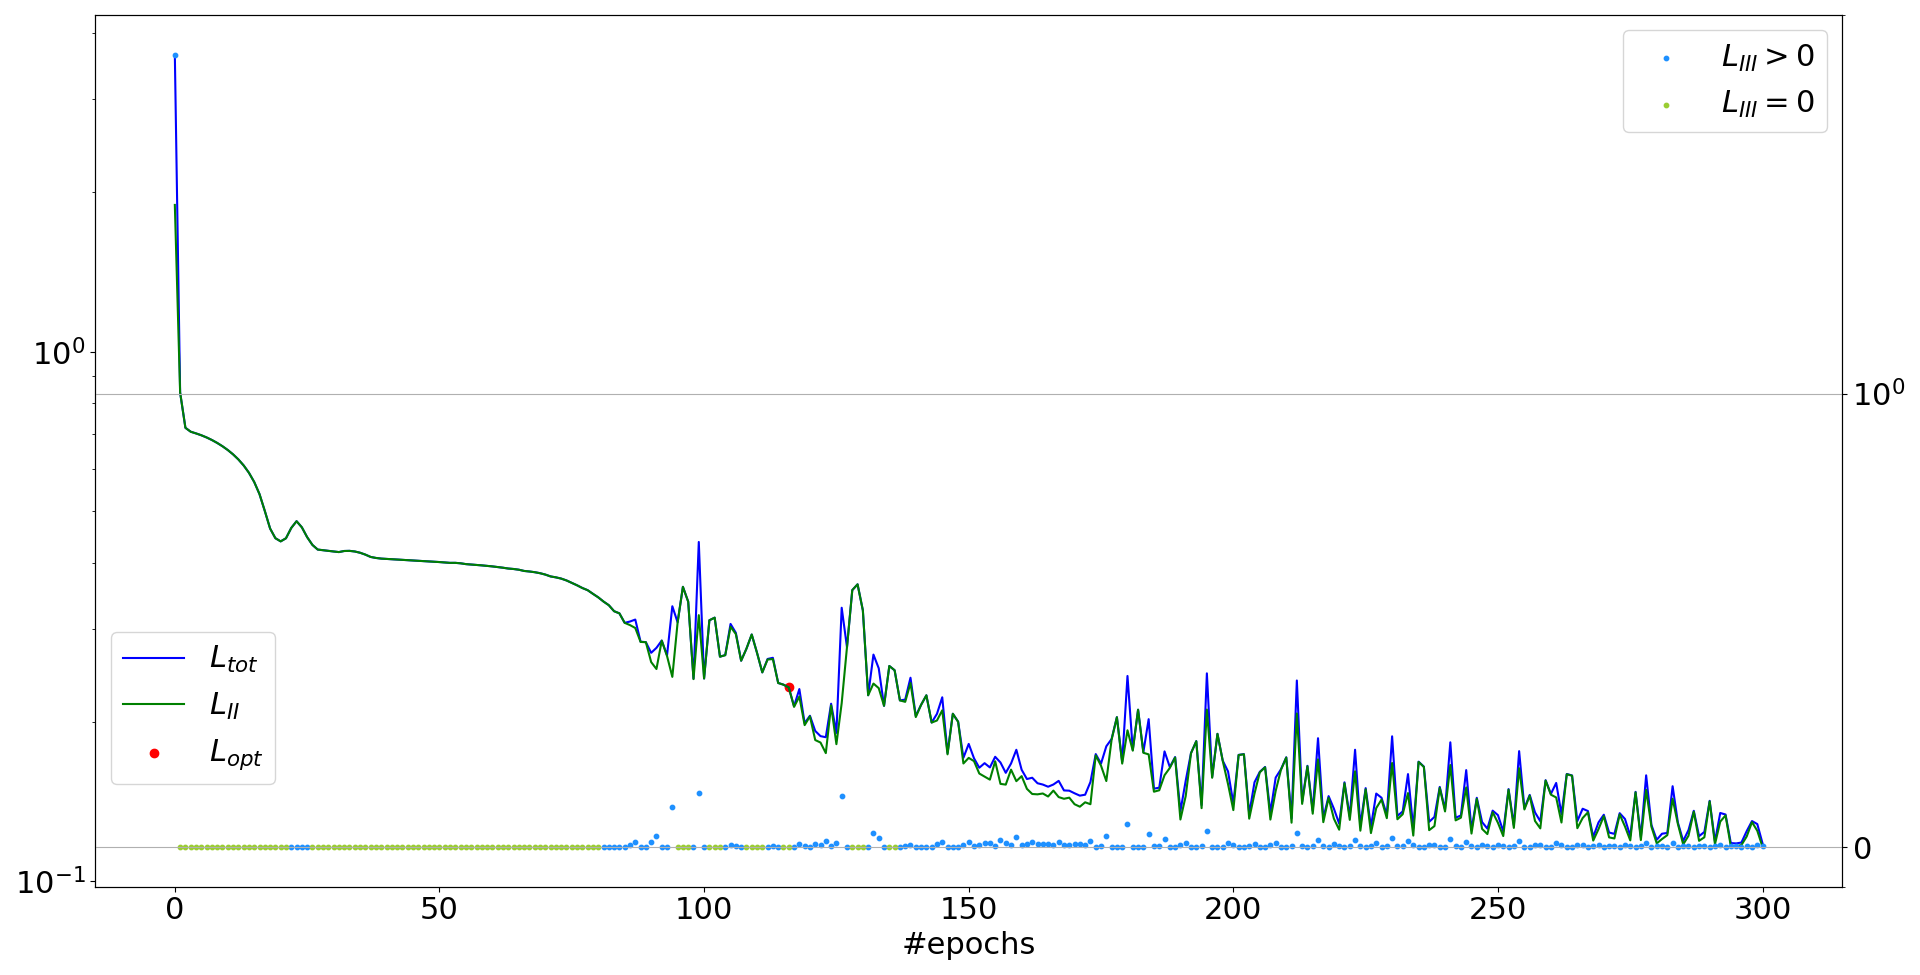
\includegraphics[width=\textwidth]{images/res_loss_exp_FGR.png}
\caption[Loss, run g]{Course of $L_{tot}$ and $L_{II}$ during training with corresponding $L_{III}$ loss values. The red point indicates lowest loss with $L_{III}=0$, run g.}
\label{fig:res_loss_exp_FGR}
\end{figure}\\
The course of the BTC was reproduced well. The largest deviations occured between $t=20 d$ and $t = 50 d$ (Fig. \ref{fig:res_btc_exp_FGR}, left).\\
FINN did not use total sorbed concentrations at the end of the experiment in the loss function because of unknown kinetical/instantaneous sorption ratios. However, the predicted course of $s_k$ at $t_{end}$ is reasonable, since $s = s_e + s_k$. Due to physical knowledge, e.g. the Freundlich sorption isotherm, $s_e$ takes positive values which decrease with decreasing $c$. It is plausible that $s_e$ is the remaining difference between $s$ and $s_k$ (Fig. \ref{fig:res_btc_exp_FGR}, right).
\begin{figure}[h!]
	\centering
	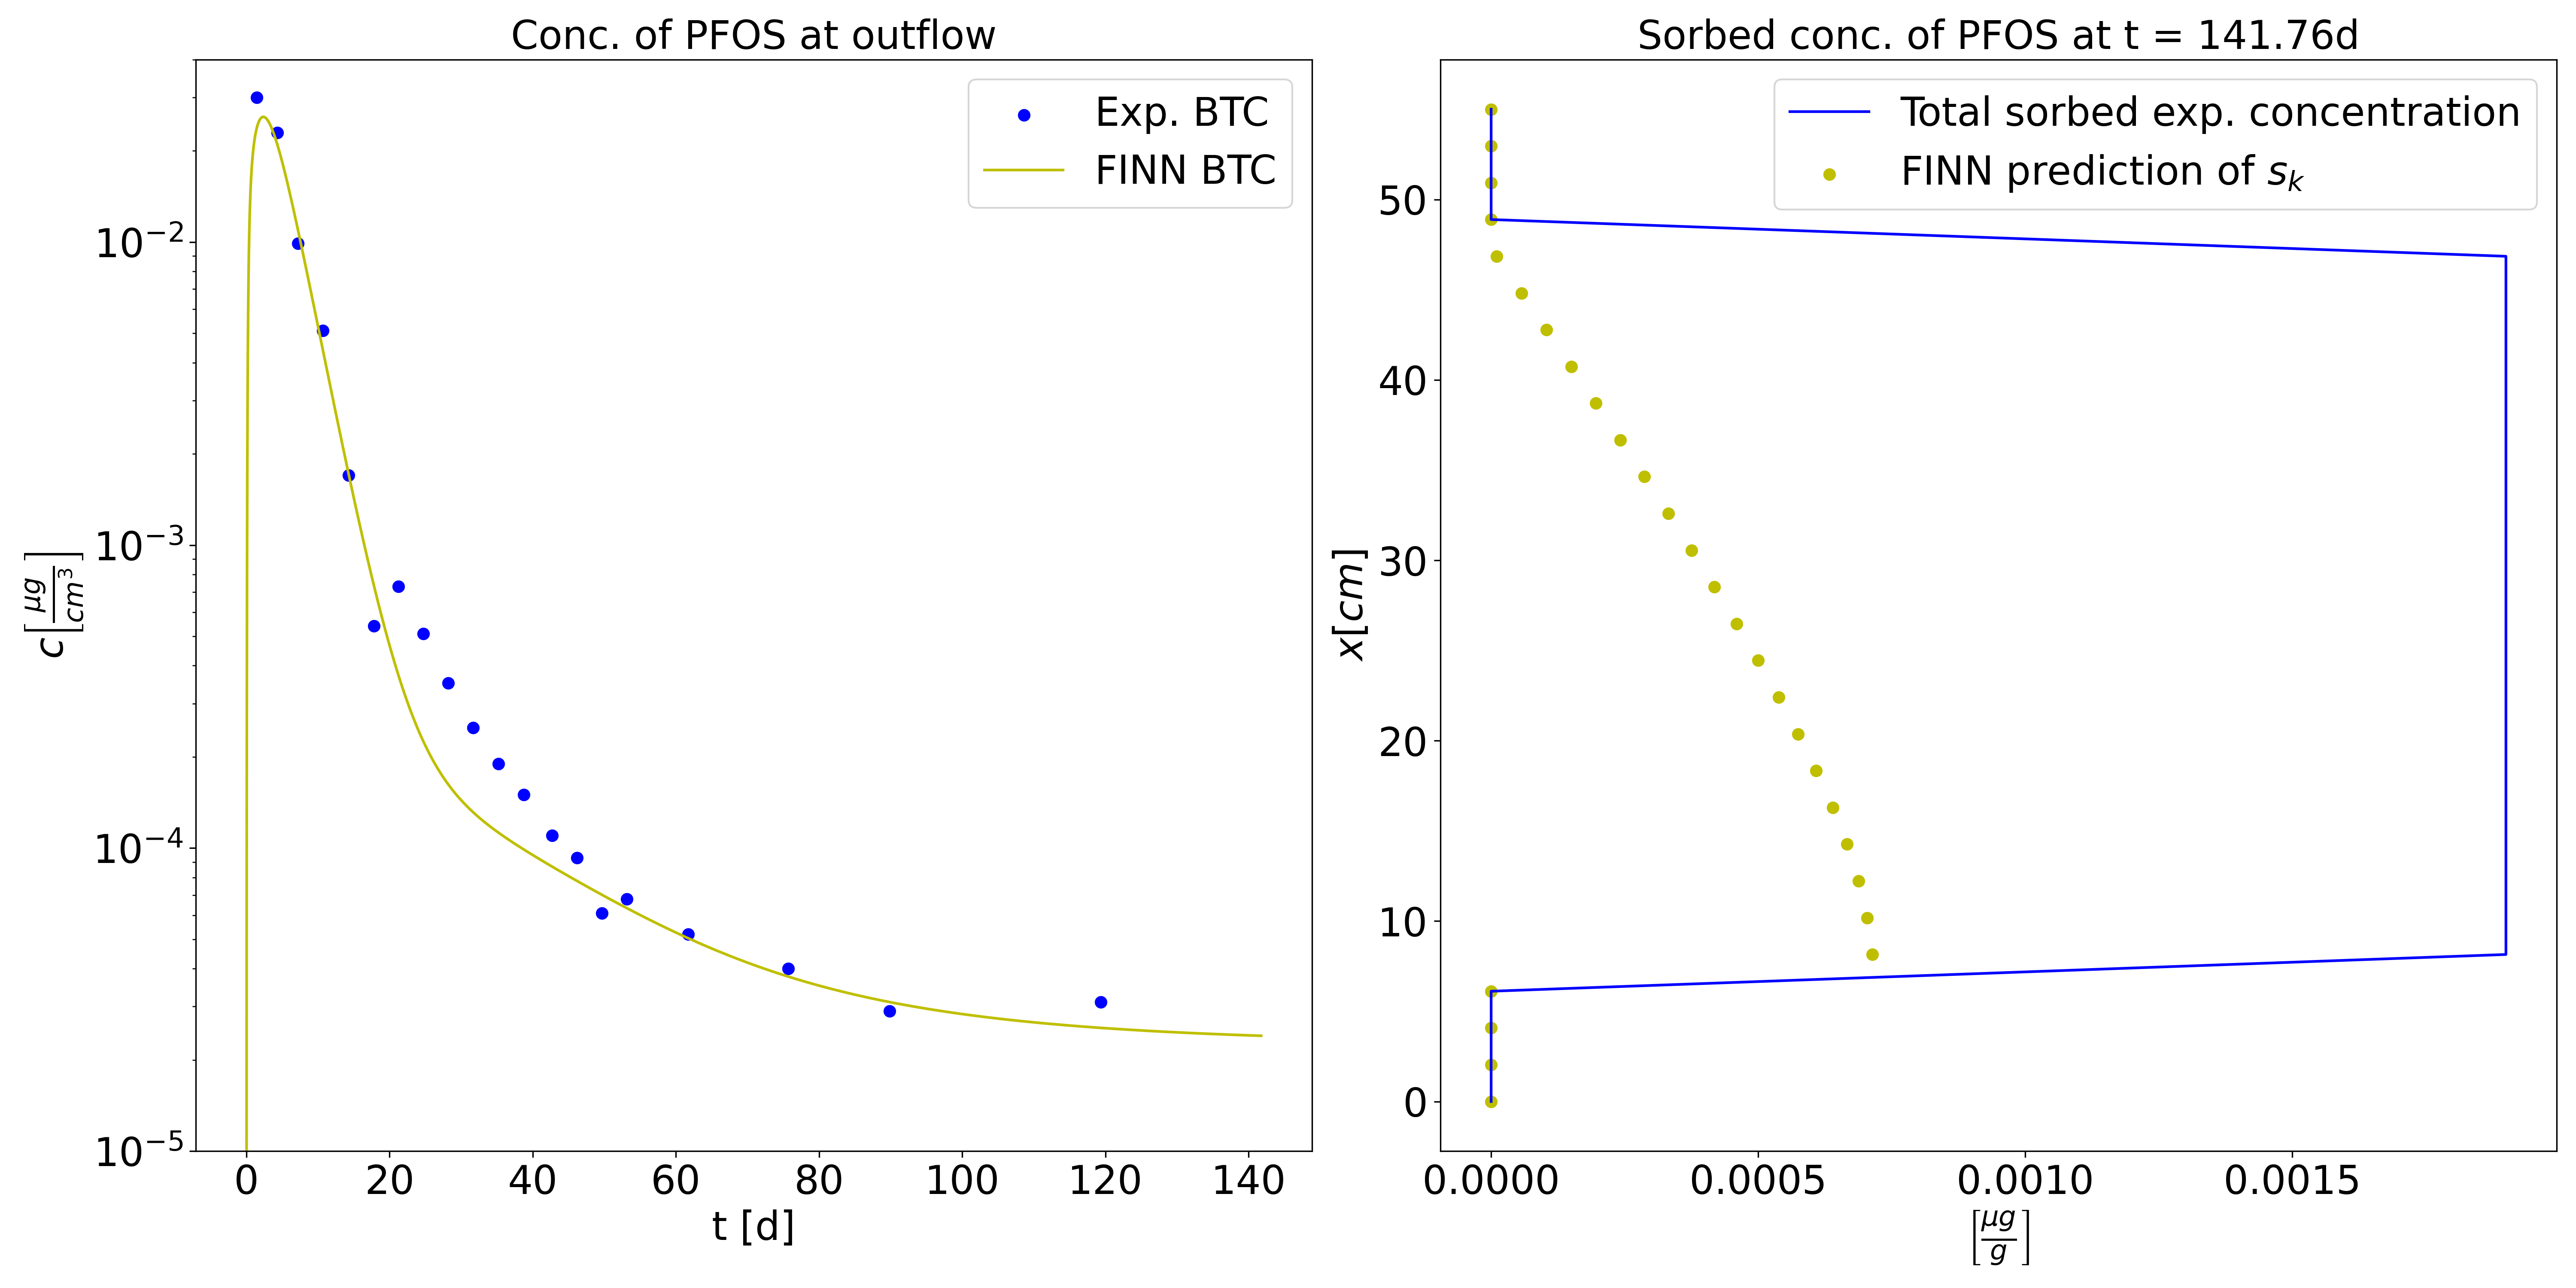
\includegraphics[width=\textwidth]{images/res_btc_exp_FGR.png}
\caption[FINN predicted BTC, run g]{BTC approximation after training with time-dependent DNNs for approximating sorption behavior using experimental BTC data (left). Comparison of FINN predicted $s_k$ and experimental total sorbed concentration $s$ at the end of the experiment (right), run g.}
\label{fig:res_btc_exp_FGR}
\end{figure}\\
\\
Experiment N1\_3 was used as \textit{out-dist} data to test the model learned from N1\_1 (Tab. \ref{tab:FGR_exp_learn}, Fig. \ref{fig:res_ov_exp_FGR_test}). The changing Darcy flux during experiment was again averaged, and varies from experiment N1\_1, which also changed advection and dispersion quantities. The initial dissolved and kinetically sorbed concentration were guessed as described in chapter 3.3.4 (Tab. \ref{tab:test_run_g}).
\begin{table}[h!]
    \centering
    \begin{tabular}{c|cccccccc}
      &$\rho_s$ & $n_{e} [-]$ &$q \left[\frac{cm}{d}\right]$ & $c_{init} \left[\frac{\mu g}{cm^3}\right] $& $s_{k,init} \left[\frac{\mu g}{g}\right]$ & $s_{k, end} \left[\frac{\mu g}{g}\right]$ & $T_{MAX} \left[d\right]$ & $T_{STEPS} \left[-\right]$ \\ [0.2 cm] \hline
      soil & 1.44 & 0.45 & 9.05 & 0.030 & 0.0098 & 0.0031 & 160 & 50000
    \end{tabular}
    \caption[Adapting parameters according to experiment N1\_3 for testing, run g]{Adapting parameters according to experiment N1\_3 for testing learned models, run g.}
    \label{tab:test_run_g}
\end{table}
\begin{figure}[h!]
	\centering
	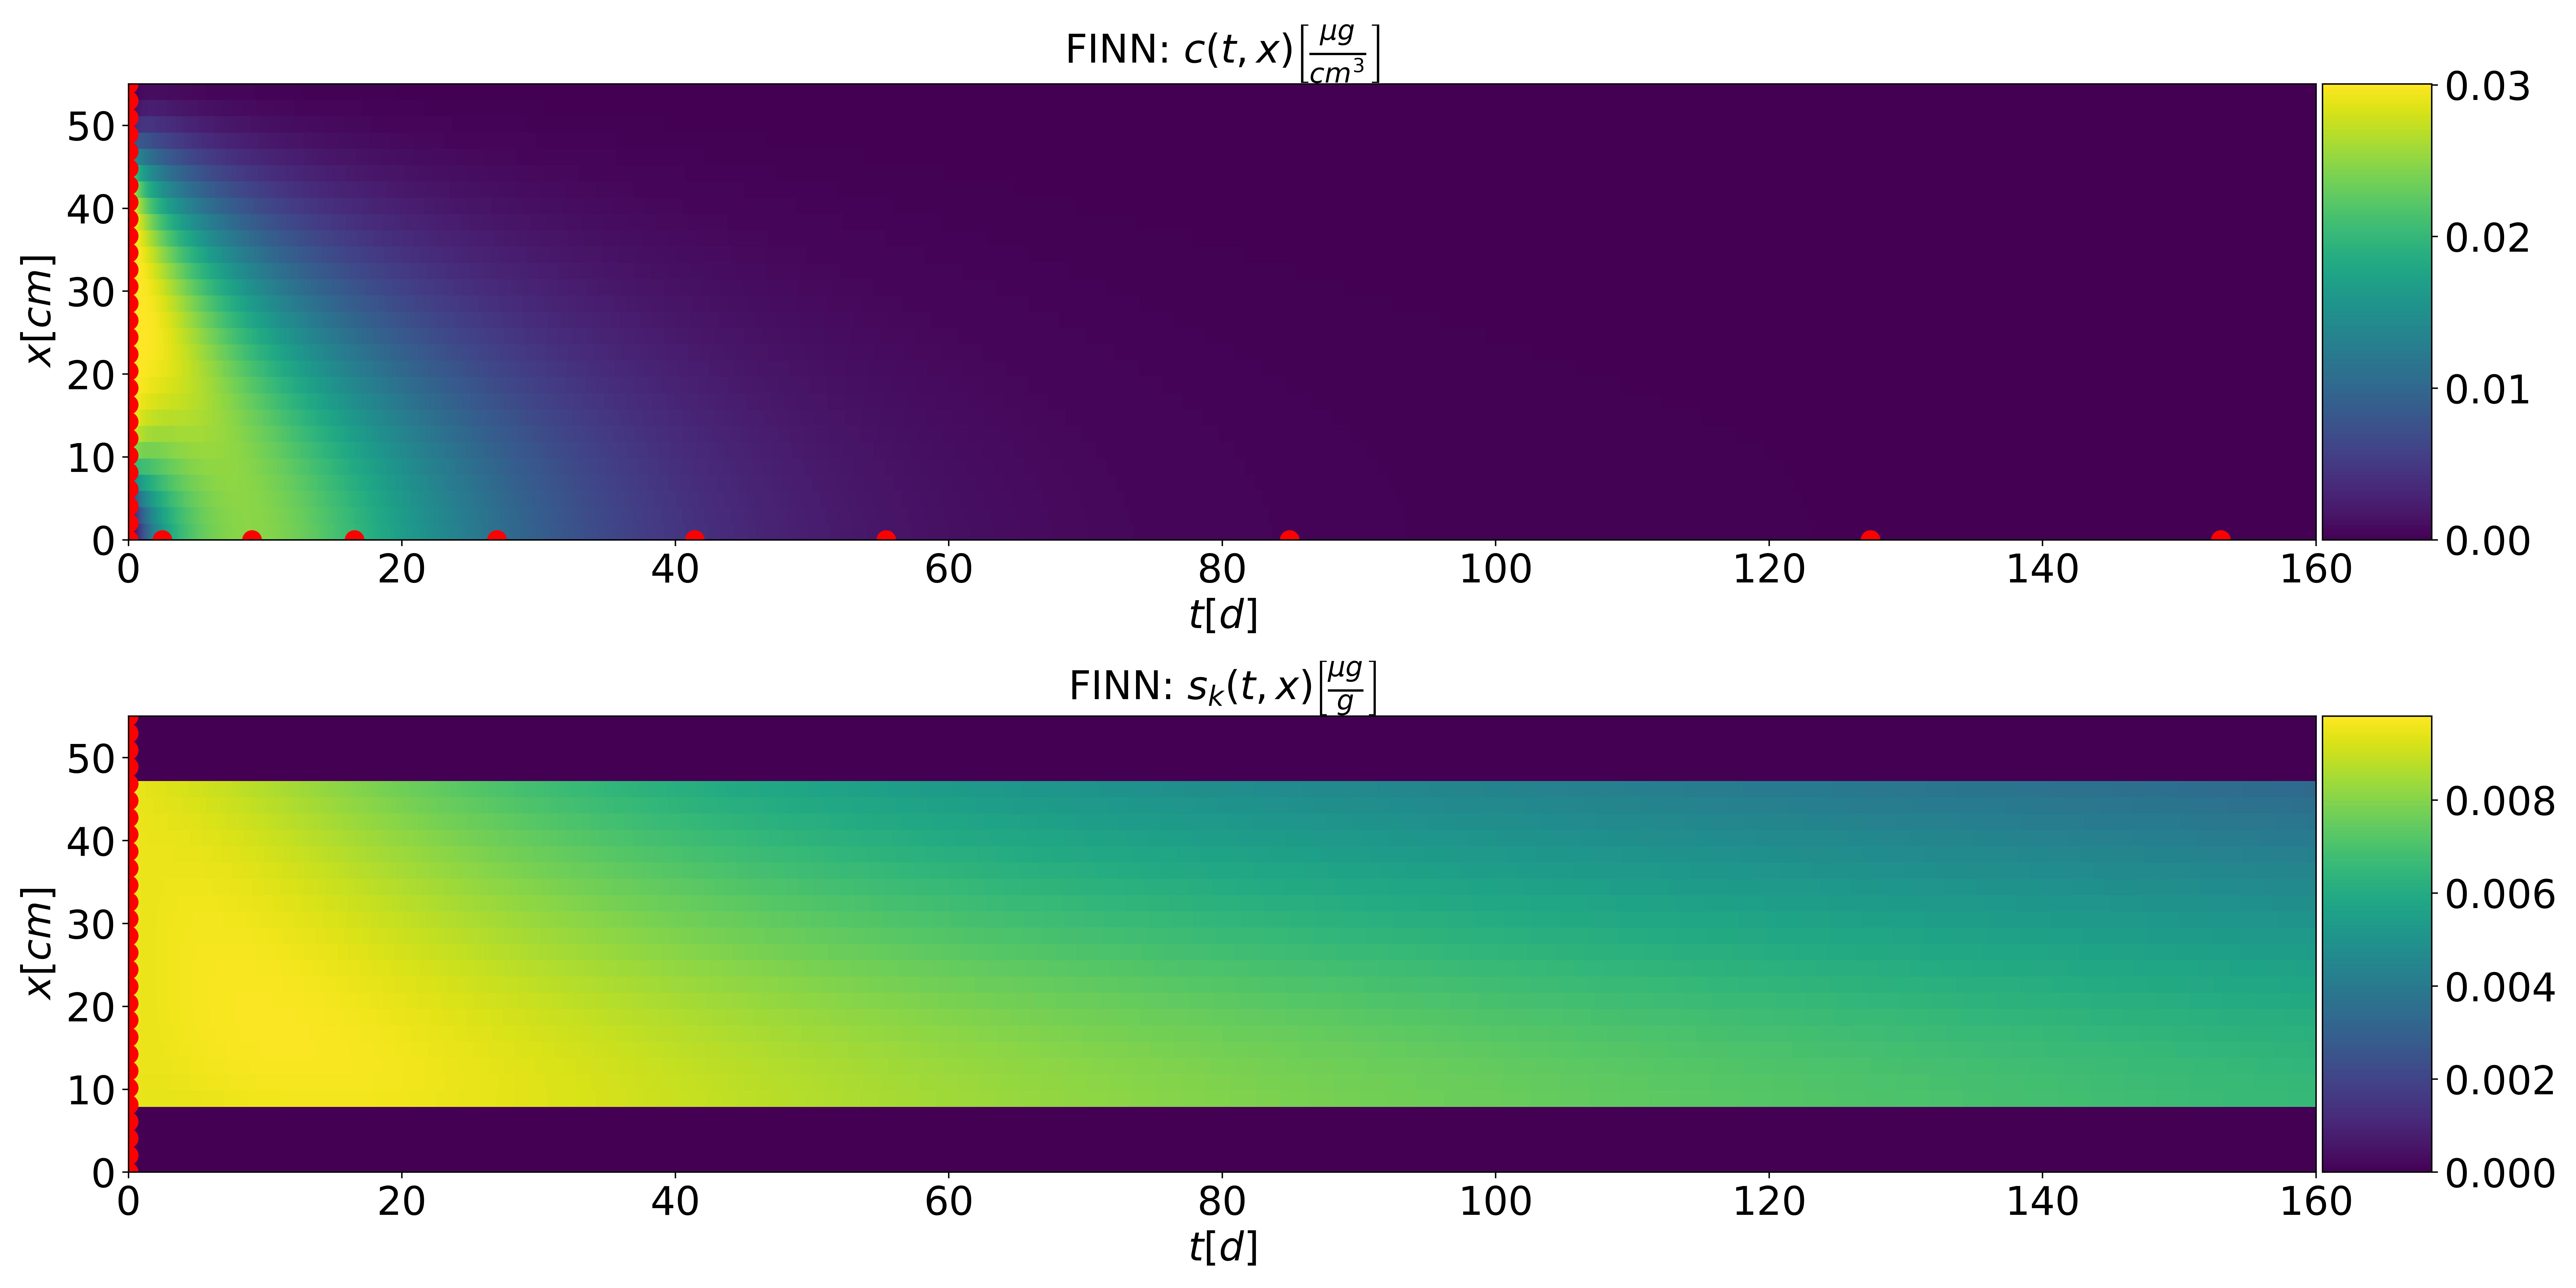
\includegraphics[width=\textwidth]{images/res_ov_exp_FGR_test.png}
\caption[FINN predicted solution after testing, run g]{FINN prediction of $c$ (top) and $s_k$ (bottom) after testing. Red points describe initial conditions and BTC concentrations of experiment N1\_3 data, which were used for the loss calculation, run g.}
\label{fig:res_ov_exp_FGR_test}
\end{figure}
\begin{table}[h!]
    \centering
    \begin{tabular}{c|c||cc}
    test & learned & \multicolumn{2}{c}{Learning schedule}\\
    \quad & scalings & $L_{II}$ & $L_{III}$ \\[0.2 cm] \hline
          $F$ & $f_{sc} = 0.0181$ & $3.60 \times 10^{-1}$ & $ 0.00 $\\
          $G$ & $g_{sc} = -0.0049$ & & \\
          $R$ & $r_{sc} = 1.0545$ & & 
        \end{tabular}
    \caption[FINN testing with unknown time-dependent functions $F$, $G$, $R$, run g]{FINN test pass with unknown time-dependent functions $F$, $G$, $R$, run g.}
    \label{tab:FGR_exp_learn}
\end{table}\\
The tested model produced good BTC results with respect to the N1\_3 experimental BTC data (Fig. \ref{fig:res_btc_exp_FGR_test}, left), but reproduced non-physical results assuming experimental data at the end of the experiment as ground truth, since $s_k > s$, (Fig. \ref{fig:res_btc_exp_FGR_test}, right).
The predicted BTCs of trainig and testing are summarized in Fig. \ref{fig:res_btc_exp_FGR_comp}.
\begin{figure}[h]
	\centering
	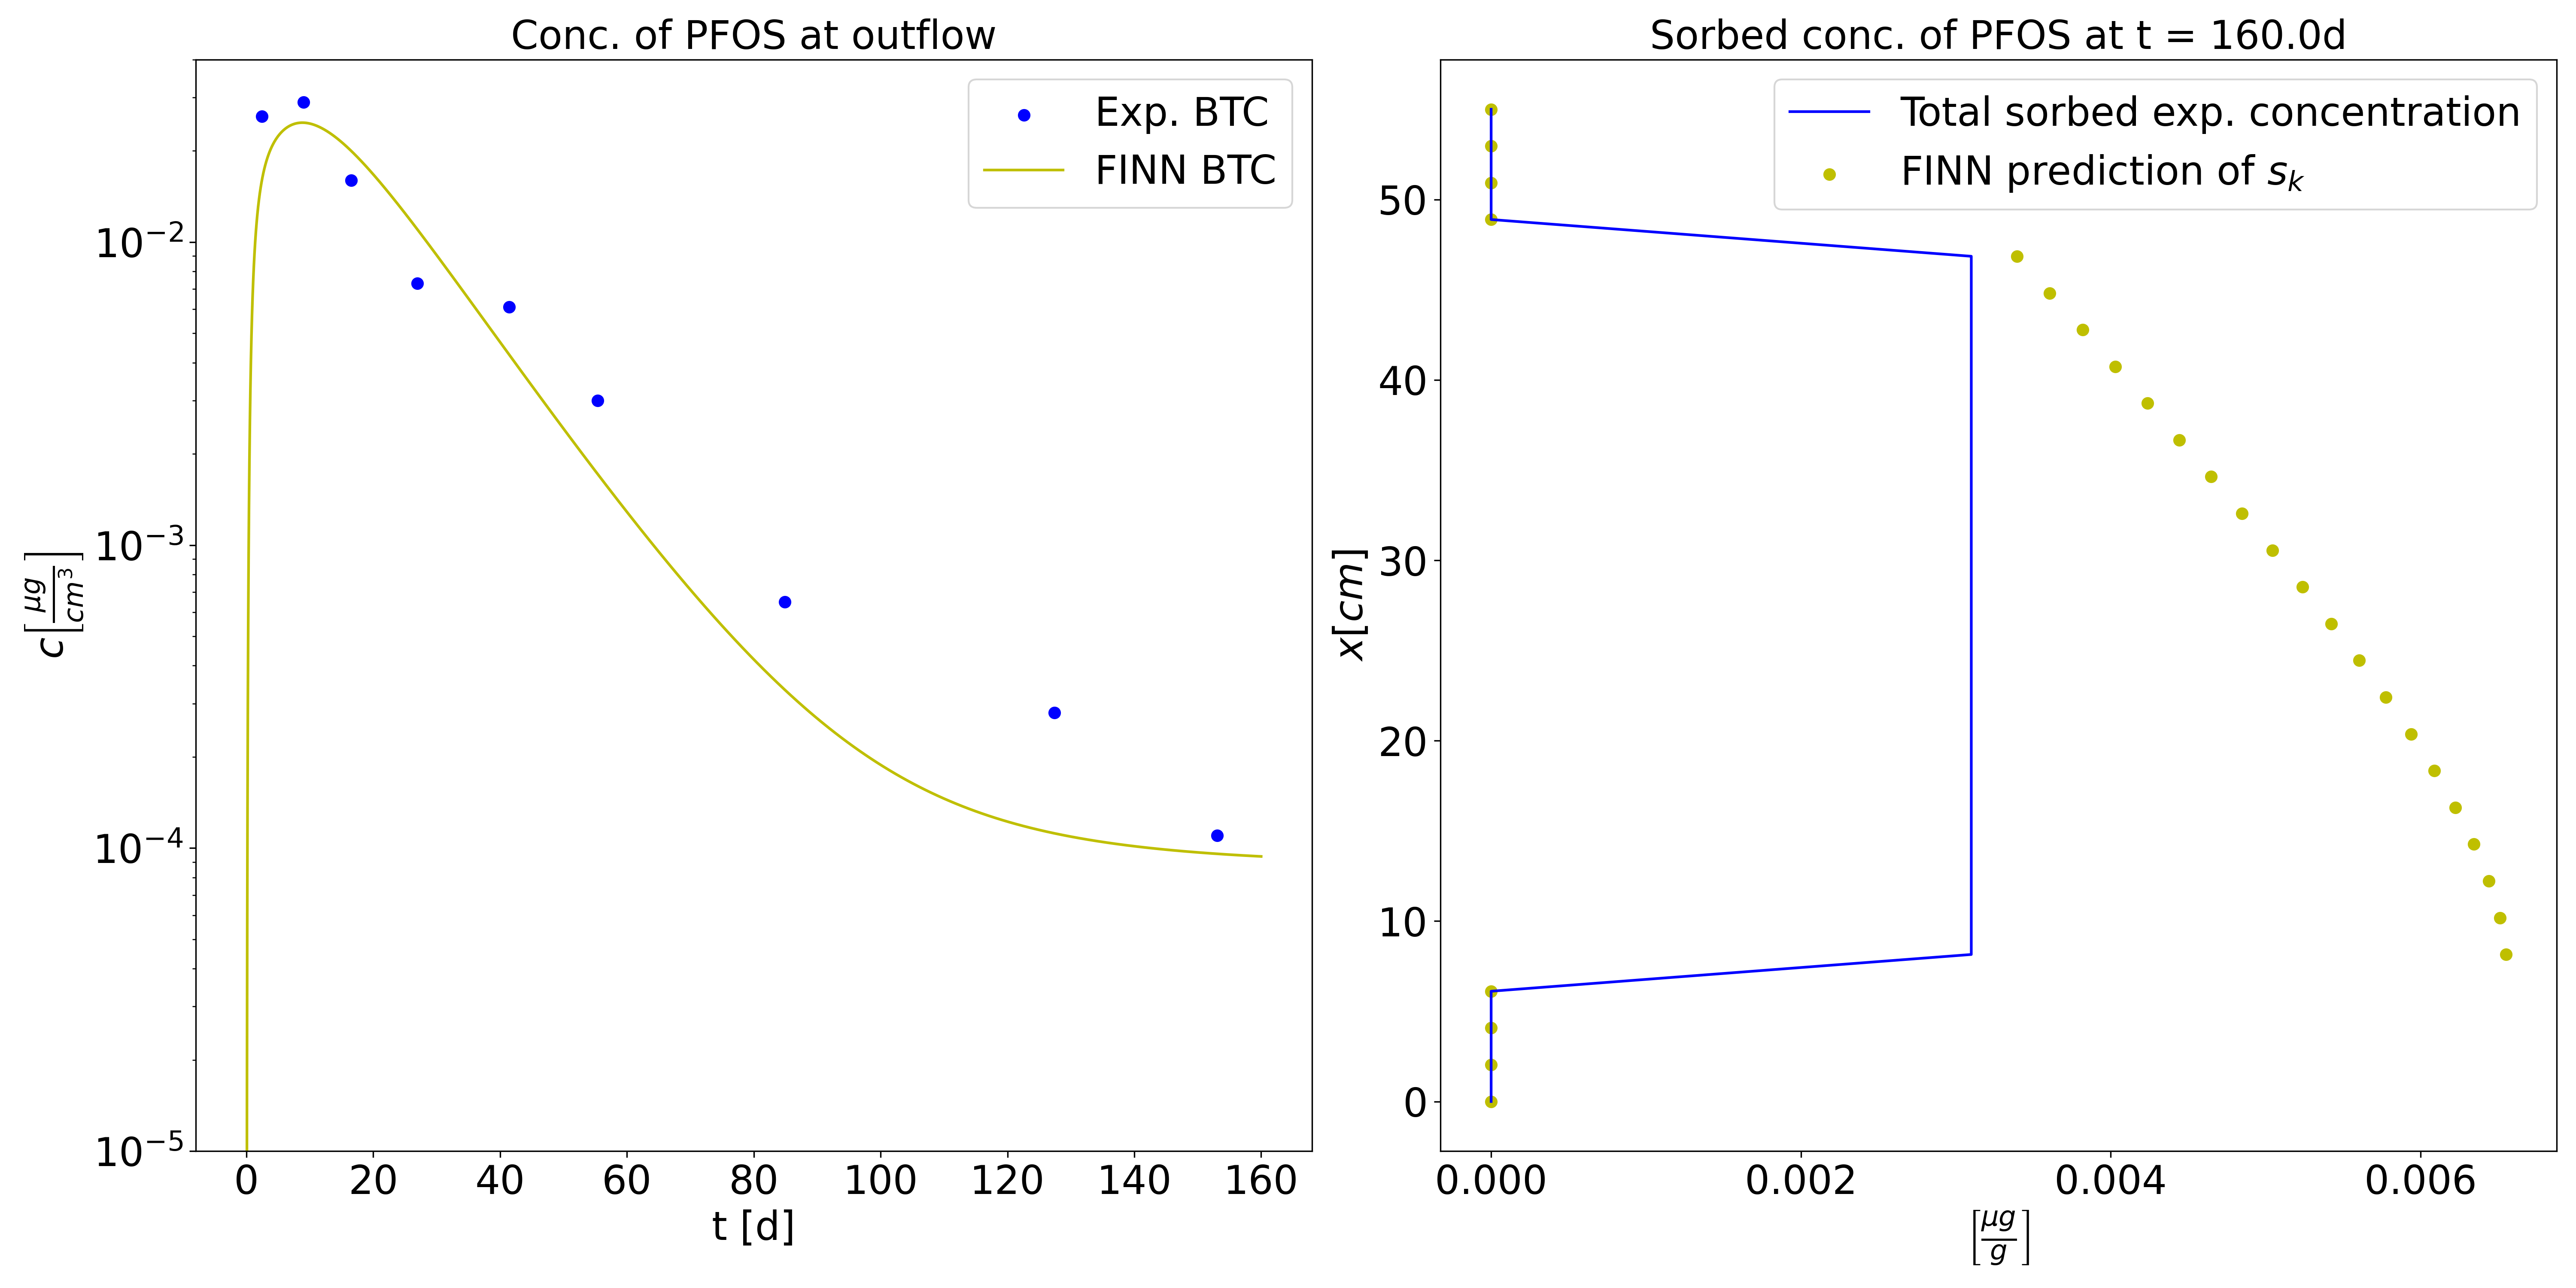
\includegraphics[width=\textwidth]{images/res_btc_exp_FGR_test.png}
\caption[FINN predicted BTC after testing, run g]{BTC approximation after \textit{out-dis-test} (left). Comparison of \textit{out-dis-test} FINN predicted $s_k$ and experimental total sorbed concentration $s$ at the end of the experiment N1\_3 (right), run g.}
\label{fig:res_btc_exp_FGR_test}
\end{figure}
\begin{figure}[h]
	\centering
	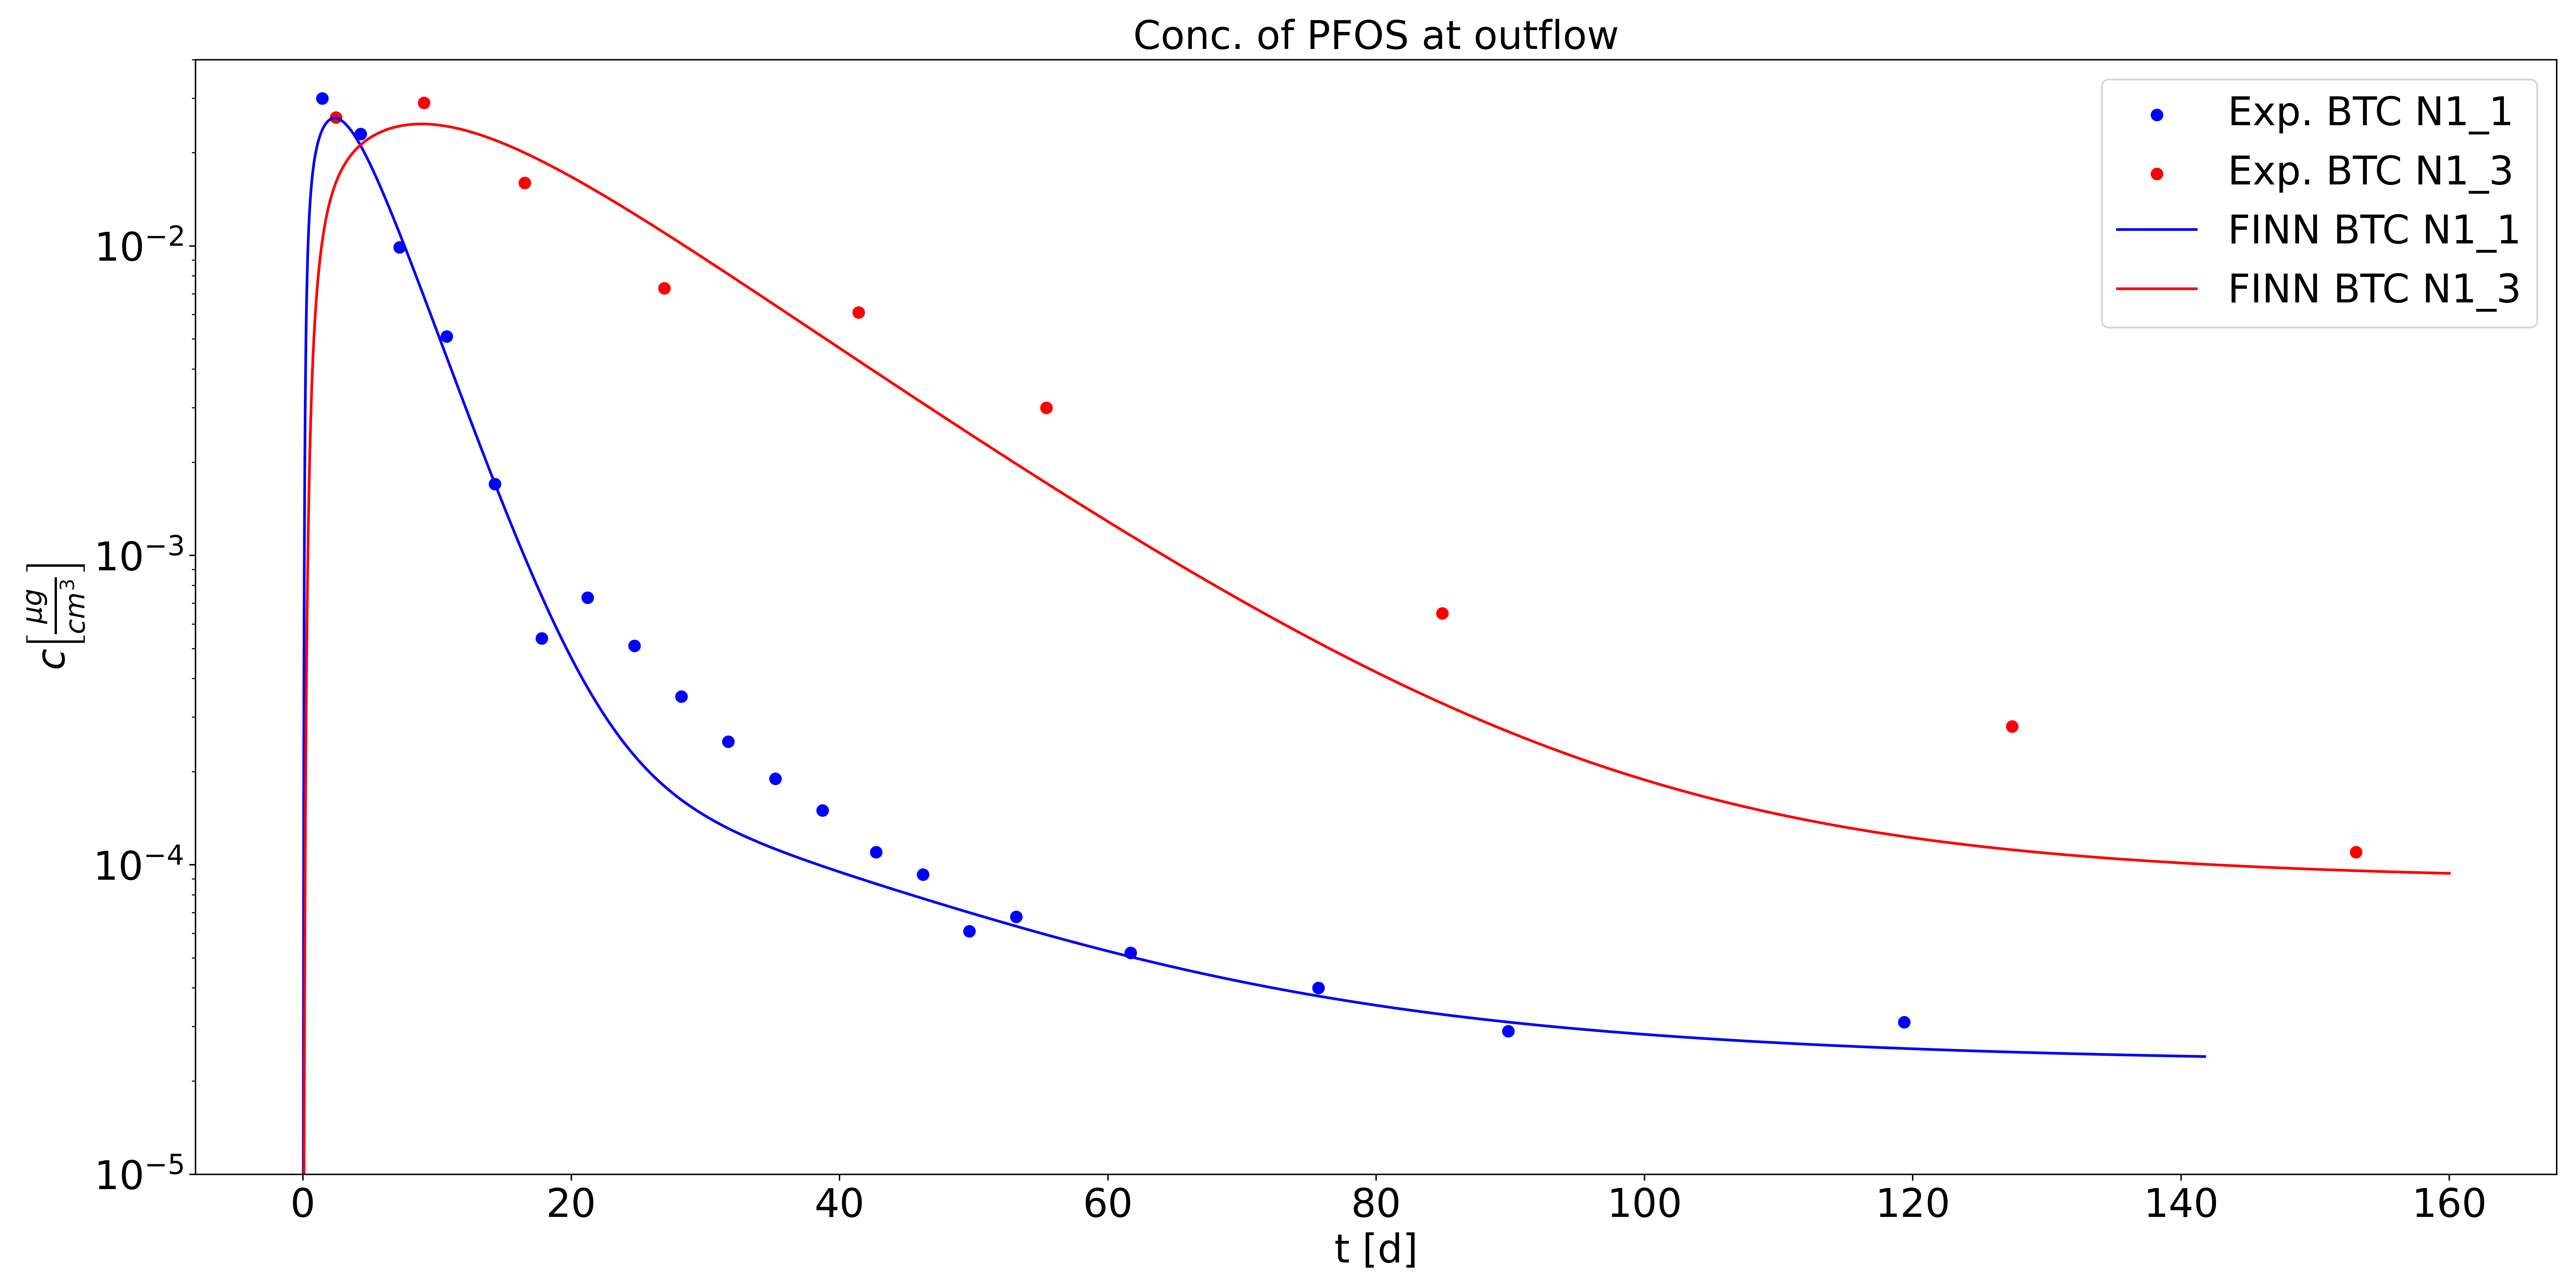
\includegraphics[width=\textwidth]{images/res_btc_exp_FGR_comp.png}
\caption[Comparison of tested and trained BTCs, run g]{Comparison of FINN predicted BTCs: Model trained with experiment N1\_1 (blue) and tested with experiment N1\_3 (red), run g.}
\label{fig:res_btc_exp_FGR_comp}
\end{figure}
\FloatBarrier
\\
\\
\textbf{Run h - Learn Time-independent $F$, $G$ and $R$}\\
In a final scenario, only implicit time-dependent $F$, $G$ and $R$ were approximated (Tab. \ref{tab:FGR_exp_indp}). The implicity is given because of the time dependency of $c$ and $s_k$ respectively.
\begin{table}[h!]
    \centering
    \begin{tabular}{c|c||cccc}
    train & init & \multicolumn{4}{c}{Learning schedule}\\
    learn & scalings & epochs & lr & $L_{II}$ & $L_{III}$ \\[0.2 cm] \hline
          $F$ & $f_{sc} = 0.1$ & 300 & 0.001 & $3.90\times 10^{-1}$ & $ 0.00 $\\
          $G$ & $g_{sc} = 0.0001$ & & & &\\
          $R$ & $r_{sc} = 1$ & & & & 
        \end{tabular}
    \caption[FINN training with unknown time-independent functions $F$, $G$, $R$, run h]{FINN training with unknown time-independent functions $F$, $G$, $R$, run h.}
    \label{tab:FGR_exp_indp}
\end{table}\\
Each function was approximated by a DNN with one input feature, one output feature, and three hidden layers with 10-20-10 neurons respectively, which leads to 
\begin{equation}
    \#\theta = \underbrace{1 \cdot 10 + 10 \cdot 20 + 20 \cdot 10 + 10 \cdot 1}_{weights} + \underbrace{10 + 20 + 10 + 1}_{bias} + \underbrace{1}_{scale} = 462
\end{equation}
parameters.\\
Again, training was done with N1\_1 experimental data (Fig. \ref{fig:res_ov_exp_FGR_indp}). As expected, run h gave slightly worse results in approximating the BTC than training the DNNs with explicit time-dependent models (run h: $L_{II} = 3.90 \times 10^{-1}$, run g: $L_{II} = 2.32 \times 10^{-1}$), (Fig. \ref{fig:res_btc_exp_FGR_indp}, left). The totally sorbed concentration at the end of the experiment was non-physically overestimated even in training (Fig. \ref{fig:res_btc_exp_FGR_indp}, right).
\begin{figure}[h!]
	\centering
	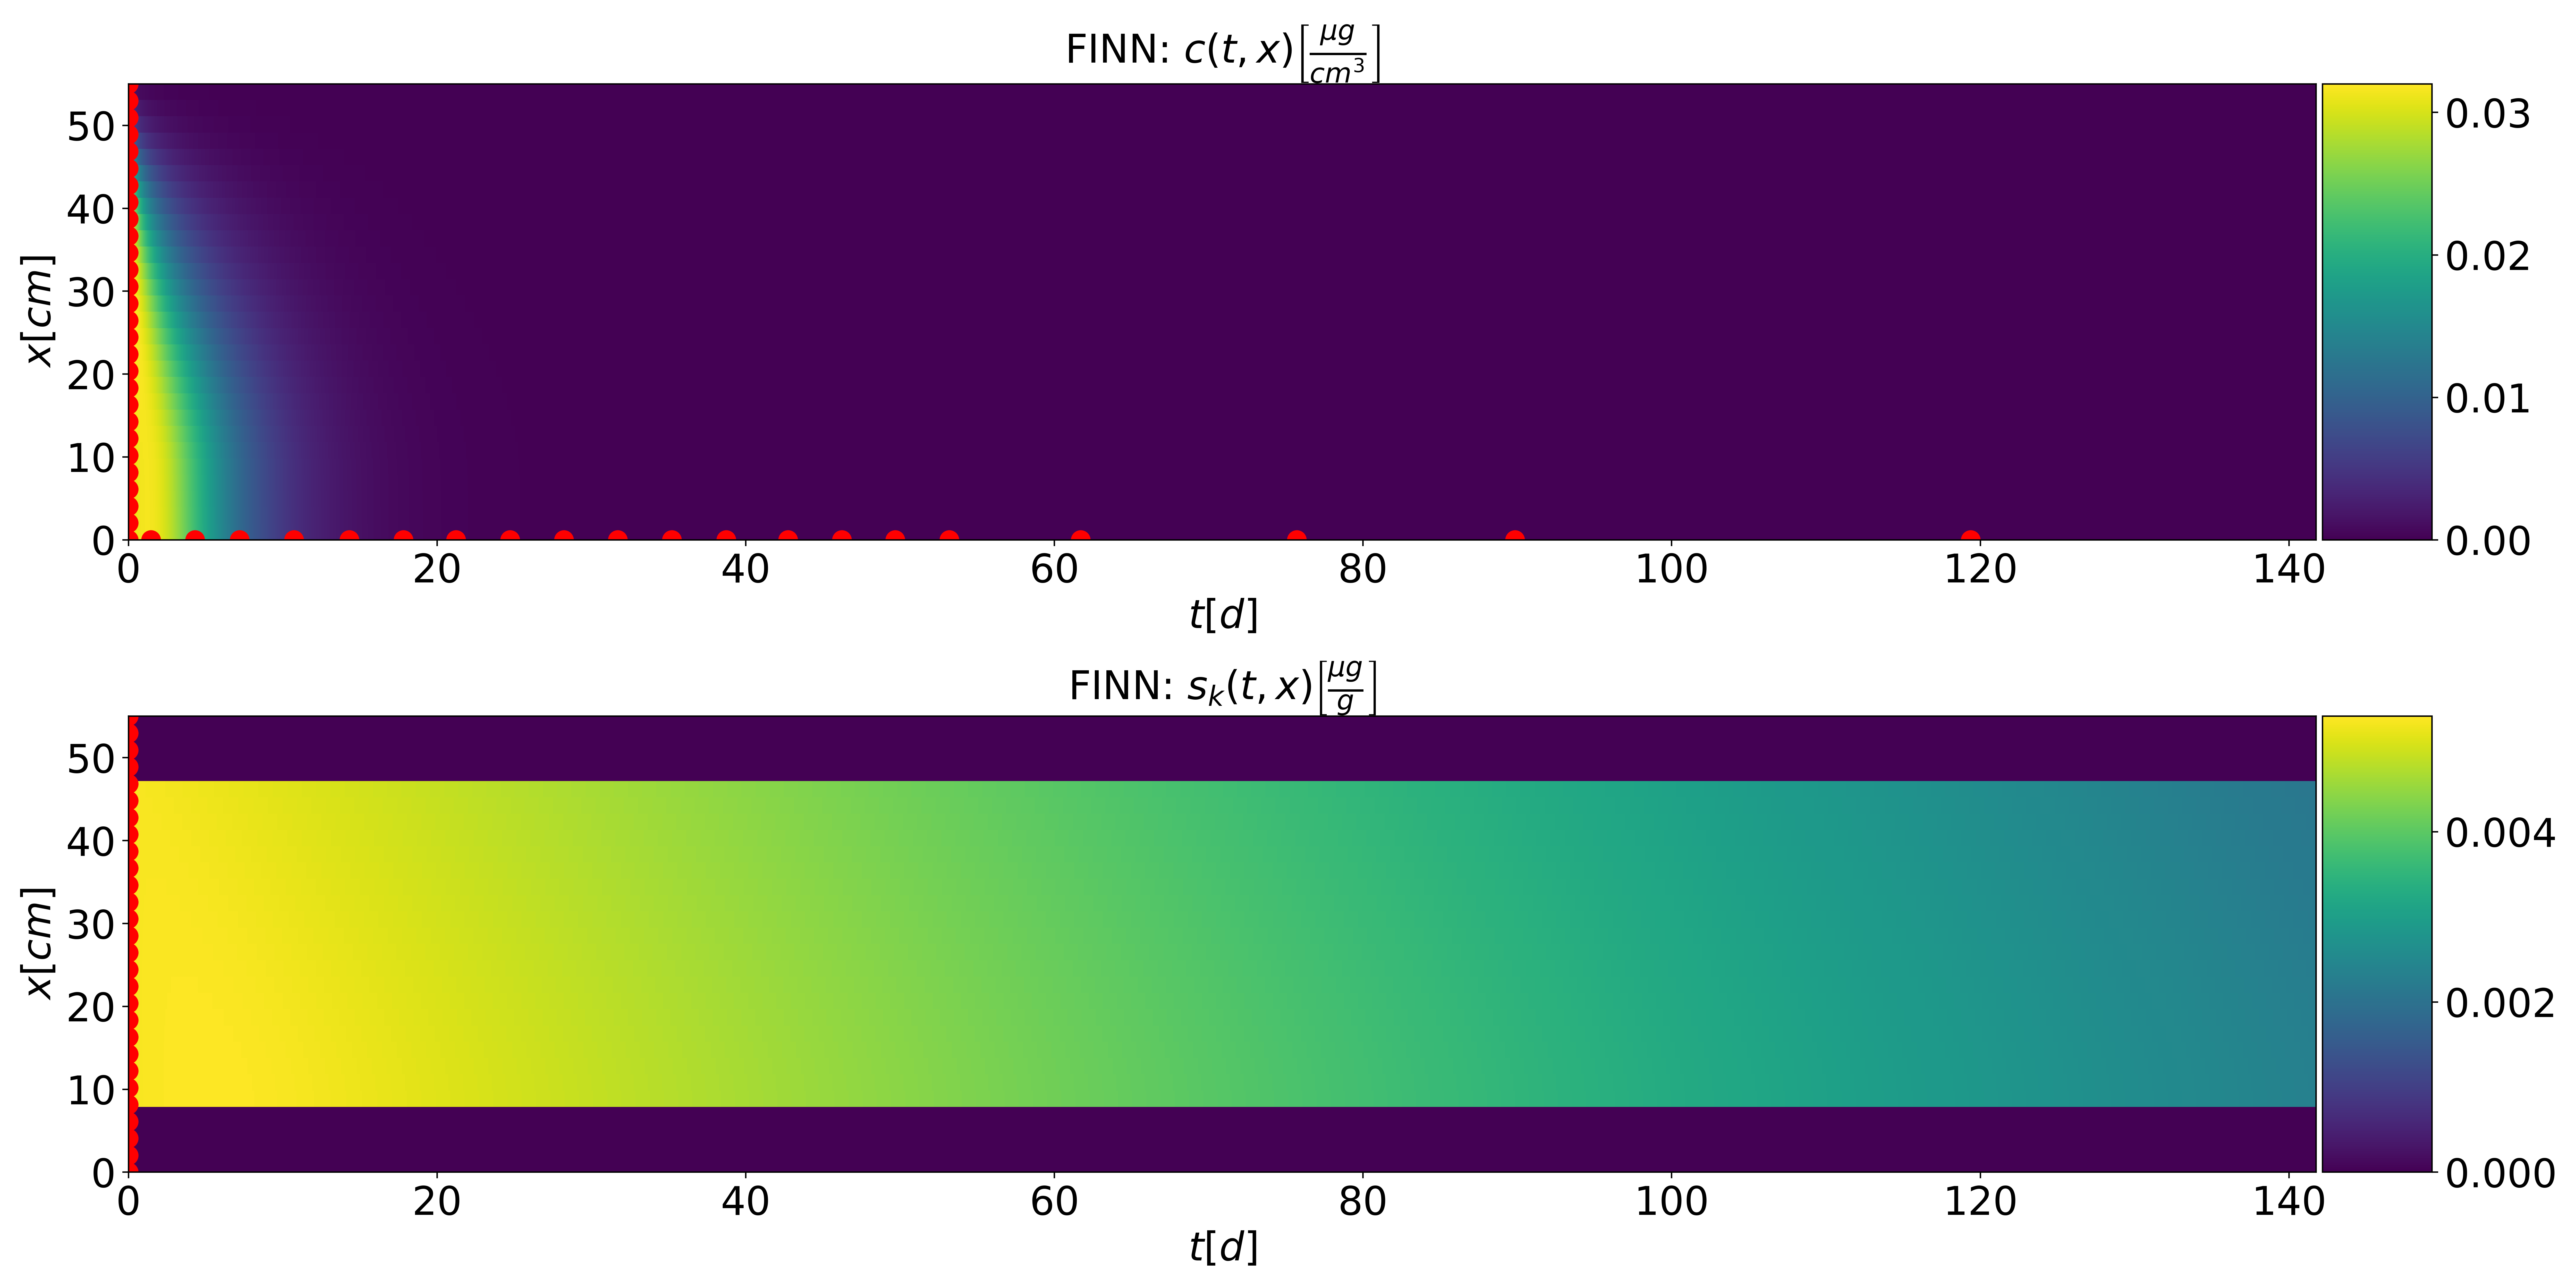
\includegraphics[width=\textwidth]{images/res_ov_exp_FGR_indp.png}
\caption[FINN predicted solution after training, run h]{FINN prediction of $c$ (top) and $s_k$ (bottom) after training time-independent functional relations. Red points describe initial conditions and BTC concentrations of experiment N1\_1 data, which were used for the loss calculation, run h.}
\label{fig:res_ov_exp_FGR_indp}
\end{figure}
\begin{figure}[h!]
	\centering
	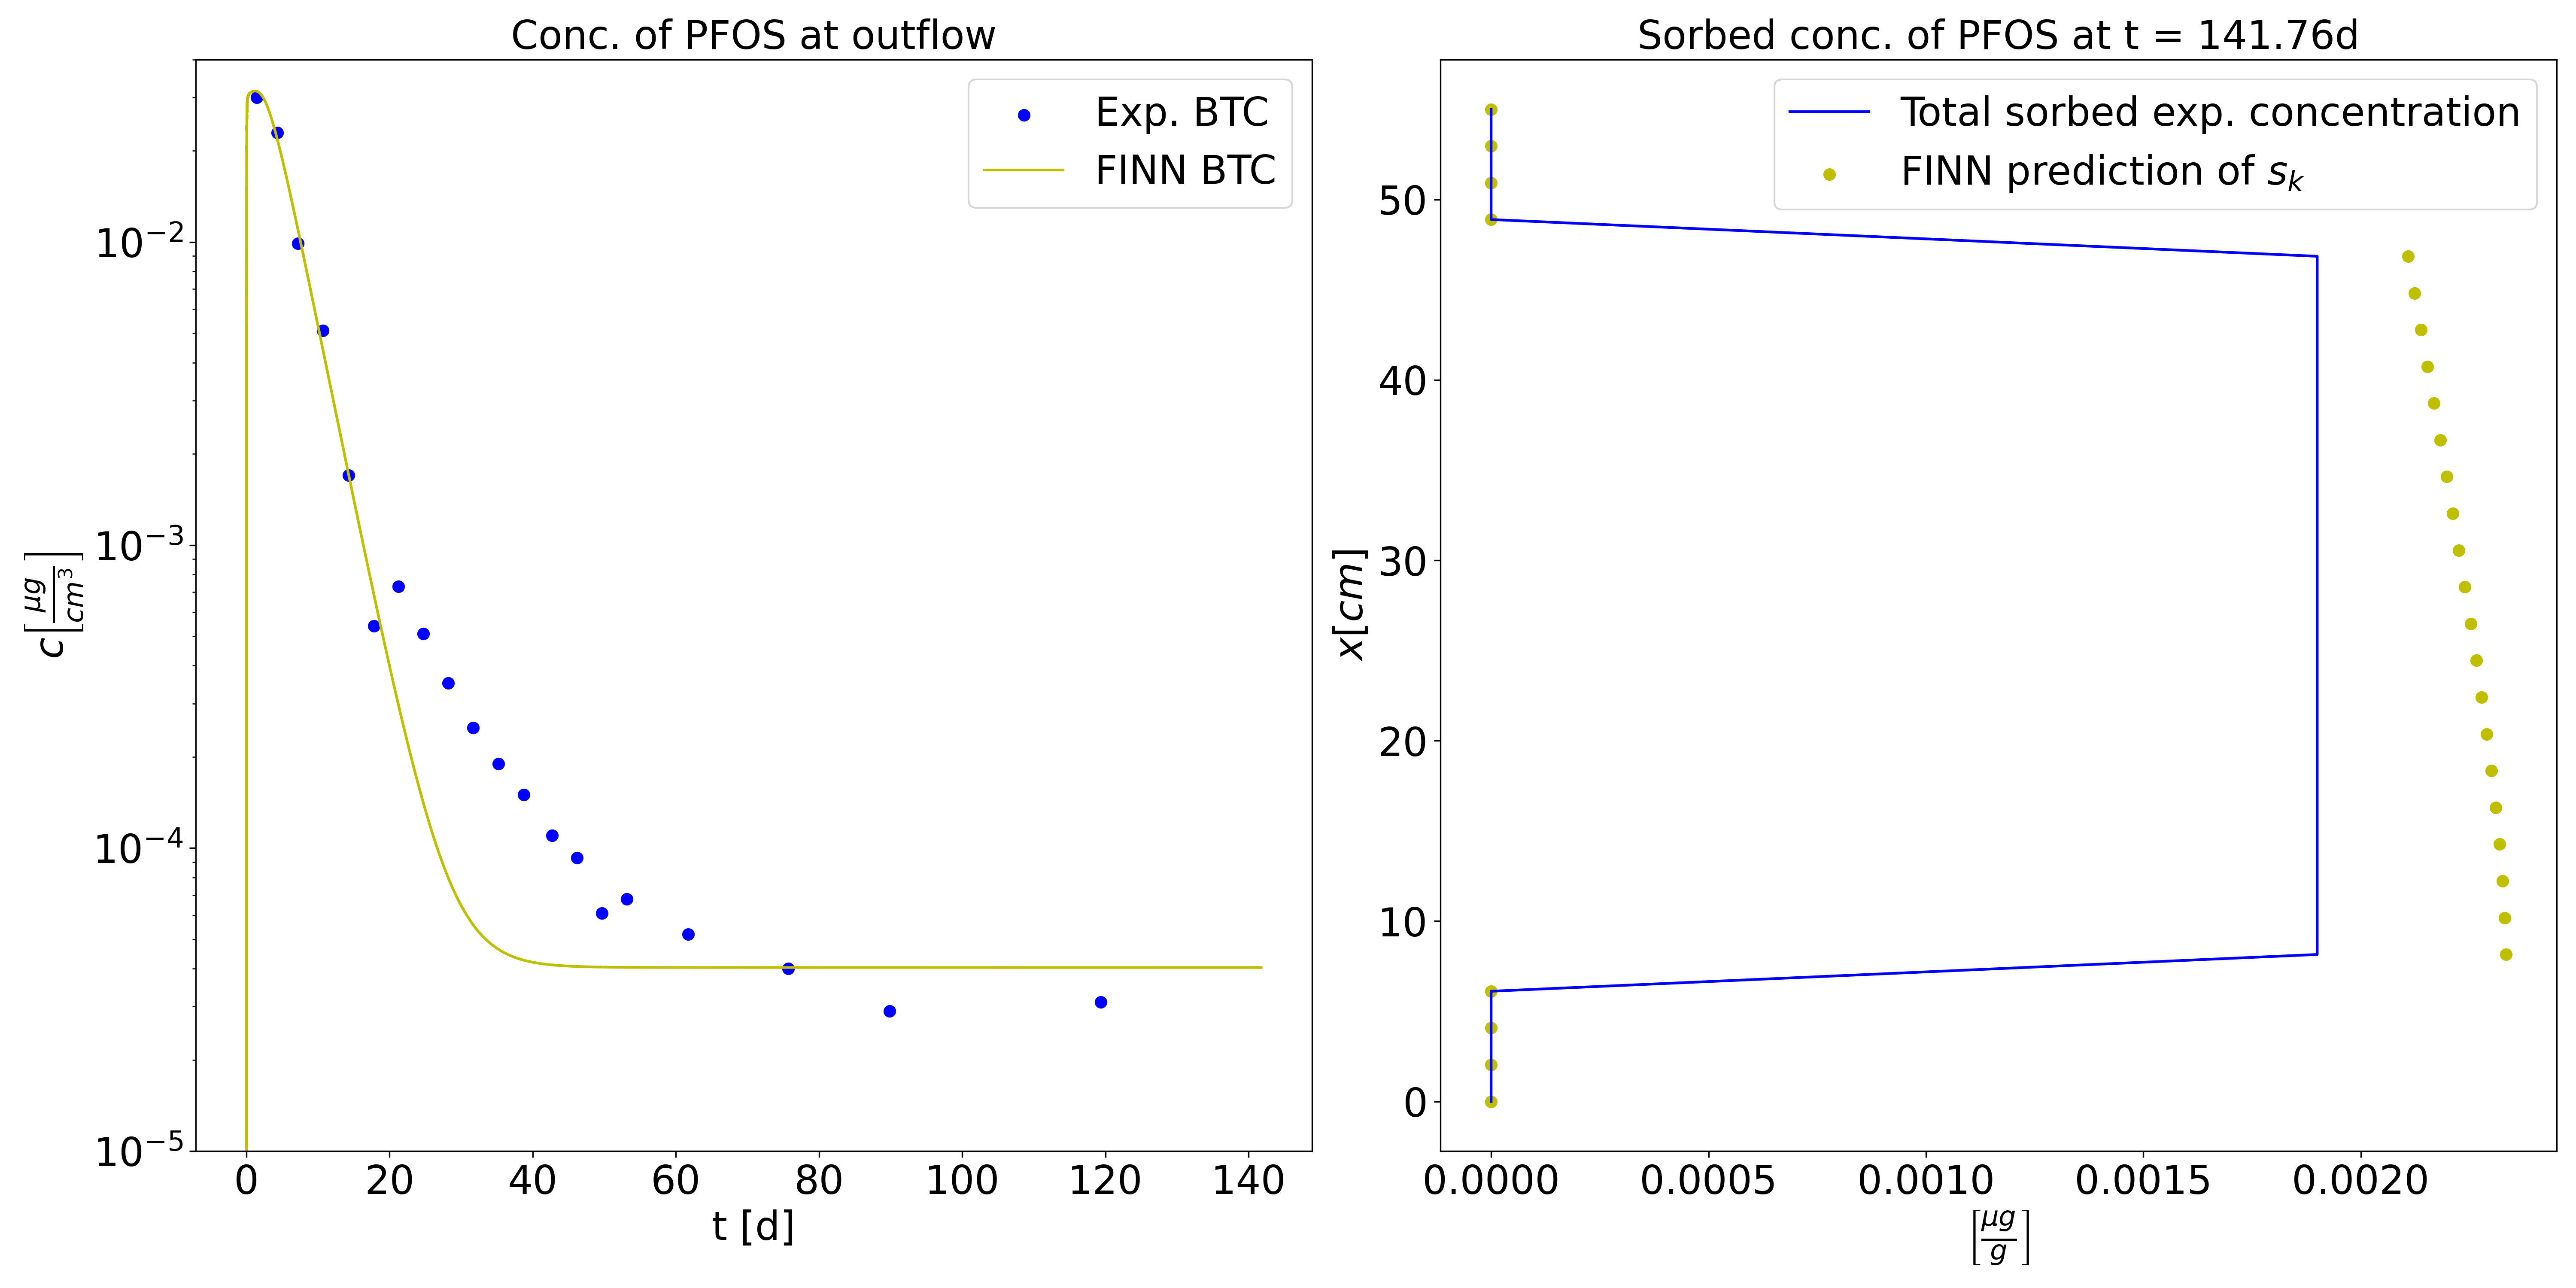
\includegraphics[width=\textwidth]{images/res_btc_exp_FGR_indp.png}
\caption[FINN predicted BTC after training, run h]{BTC approximation after training with time-independent DNNs for approximating sorption behavior using experimental BTC data (left). Comparison of FINN predicted $s_k$ and experimental total sorbed concentration $s$ at the end of the experiment (right), run h.}
\label{fig:res_btc_exp_FGR_indp}
\end{figure}\\
During training, negative concentrations were learned only in very few epochs (Fig. \ref{fig:res_loss_exp_FGR_indp}). The order of magnitude of the punishment factor included in $L_{III}$ is reasonably chosen here. Since the loss value remained roughly constant over the last 150 epochs, a lower learning rate might have been used.
\begin{figure}[h!]
	\centering
	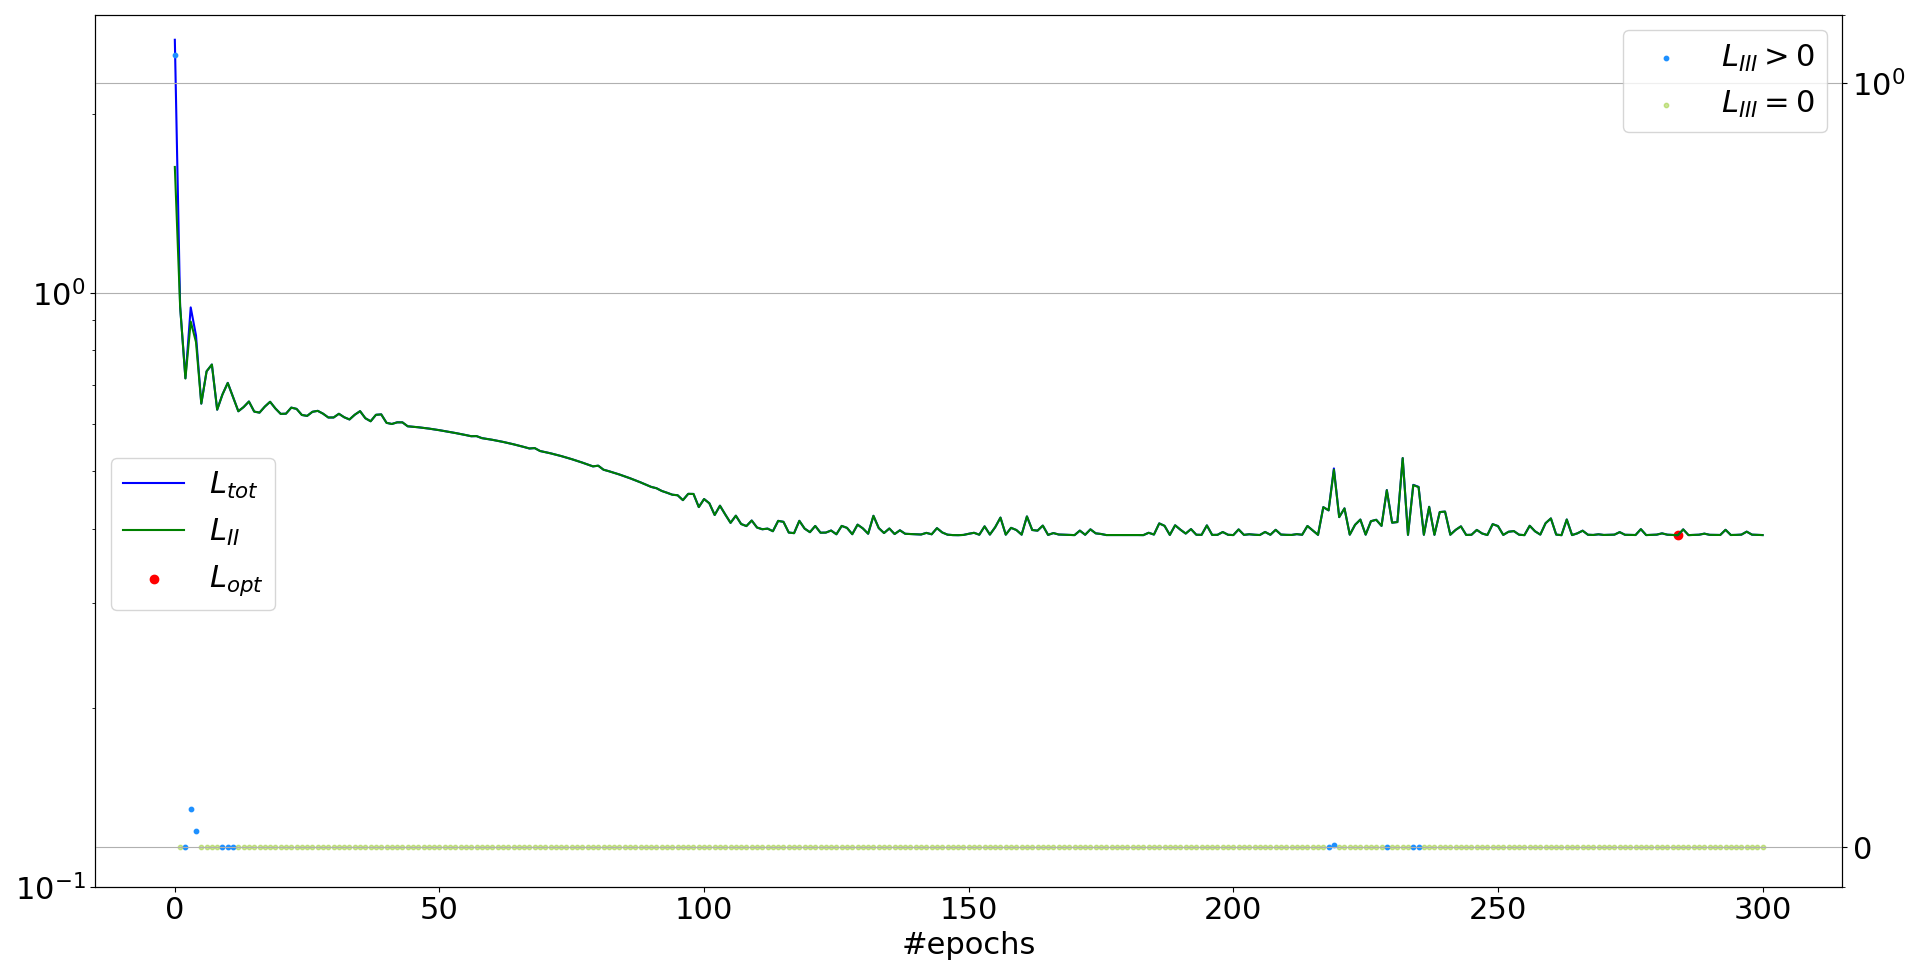
\includegraphics[width=\textwidth]{images/res_loss_exp_FGR_indp.png}
\caption[Loss, run h]{Course of $L_{tot}$ and $L_{II}$ during training with corresponding $L_{III}$ loss values. The red point indicates lowest loss with $L_{III}=0$, run h.}
\label{fig:res_loss_exp_FGR_indp}
\end{figure}\\
\\
Interestingly, the \textit{out-dis-test} with N1\_3 data (Fig. \ref{fig:res_ov_exp_FGR_test_indp}) for time-independent DNNs produced good results at least for the approximation of the BTC (Fig. \ref{fig:res_btc_exp_FGR_test_indp}, left). Again, $s_k$ was overestimated at the end of the experiment (Fig. \ref{fig:res_btc_exp_FGR_test_indp}, right).
\begin{table}[h!]
    \centering
    \begin{tabular}{c|c||cc}
    test & learned & \multicolumn{2}{c}{Learning schedule}\\
    \quad & scalings & $L_{II}$ & $L_{III}$ \\[0.2 cm] \hline
          $F$ & $f_{sc} = 0.0089$ & $3.30 \times 10^{-1}$ & $ 0.00 $\\
          $G$ & $g_{sc} = -0.0003$ & & \\
          $R$ & $r_{sc} = 1.1673$ & & 
        \end{tabular}
    \caption[FINN testing with unknown time-independent functions $F$, $G$, $R$, run h]{FINN test pass with unknown functions $F$, $G$, $R$, run h.}
    \label{tab:FGR_exp_indp_test}
\end{table}
\begin{figure}[h!]
	\centering
	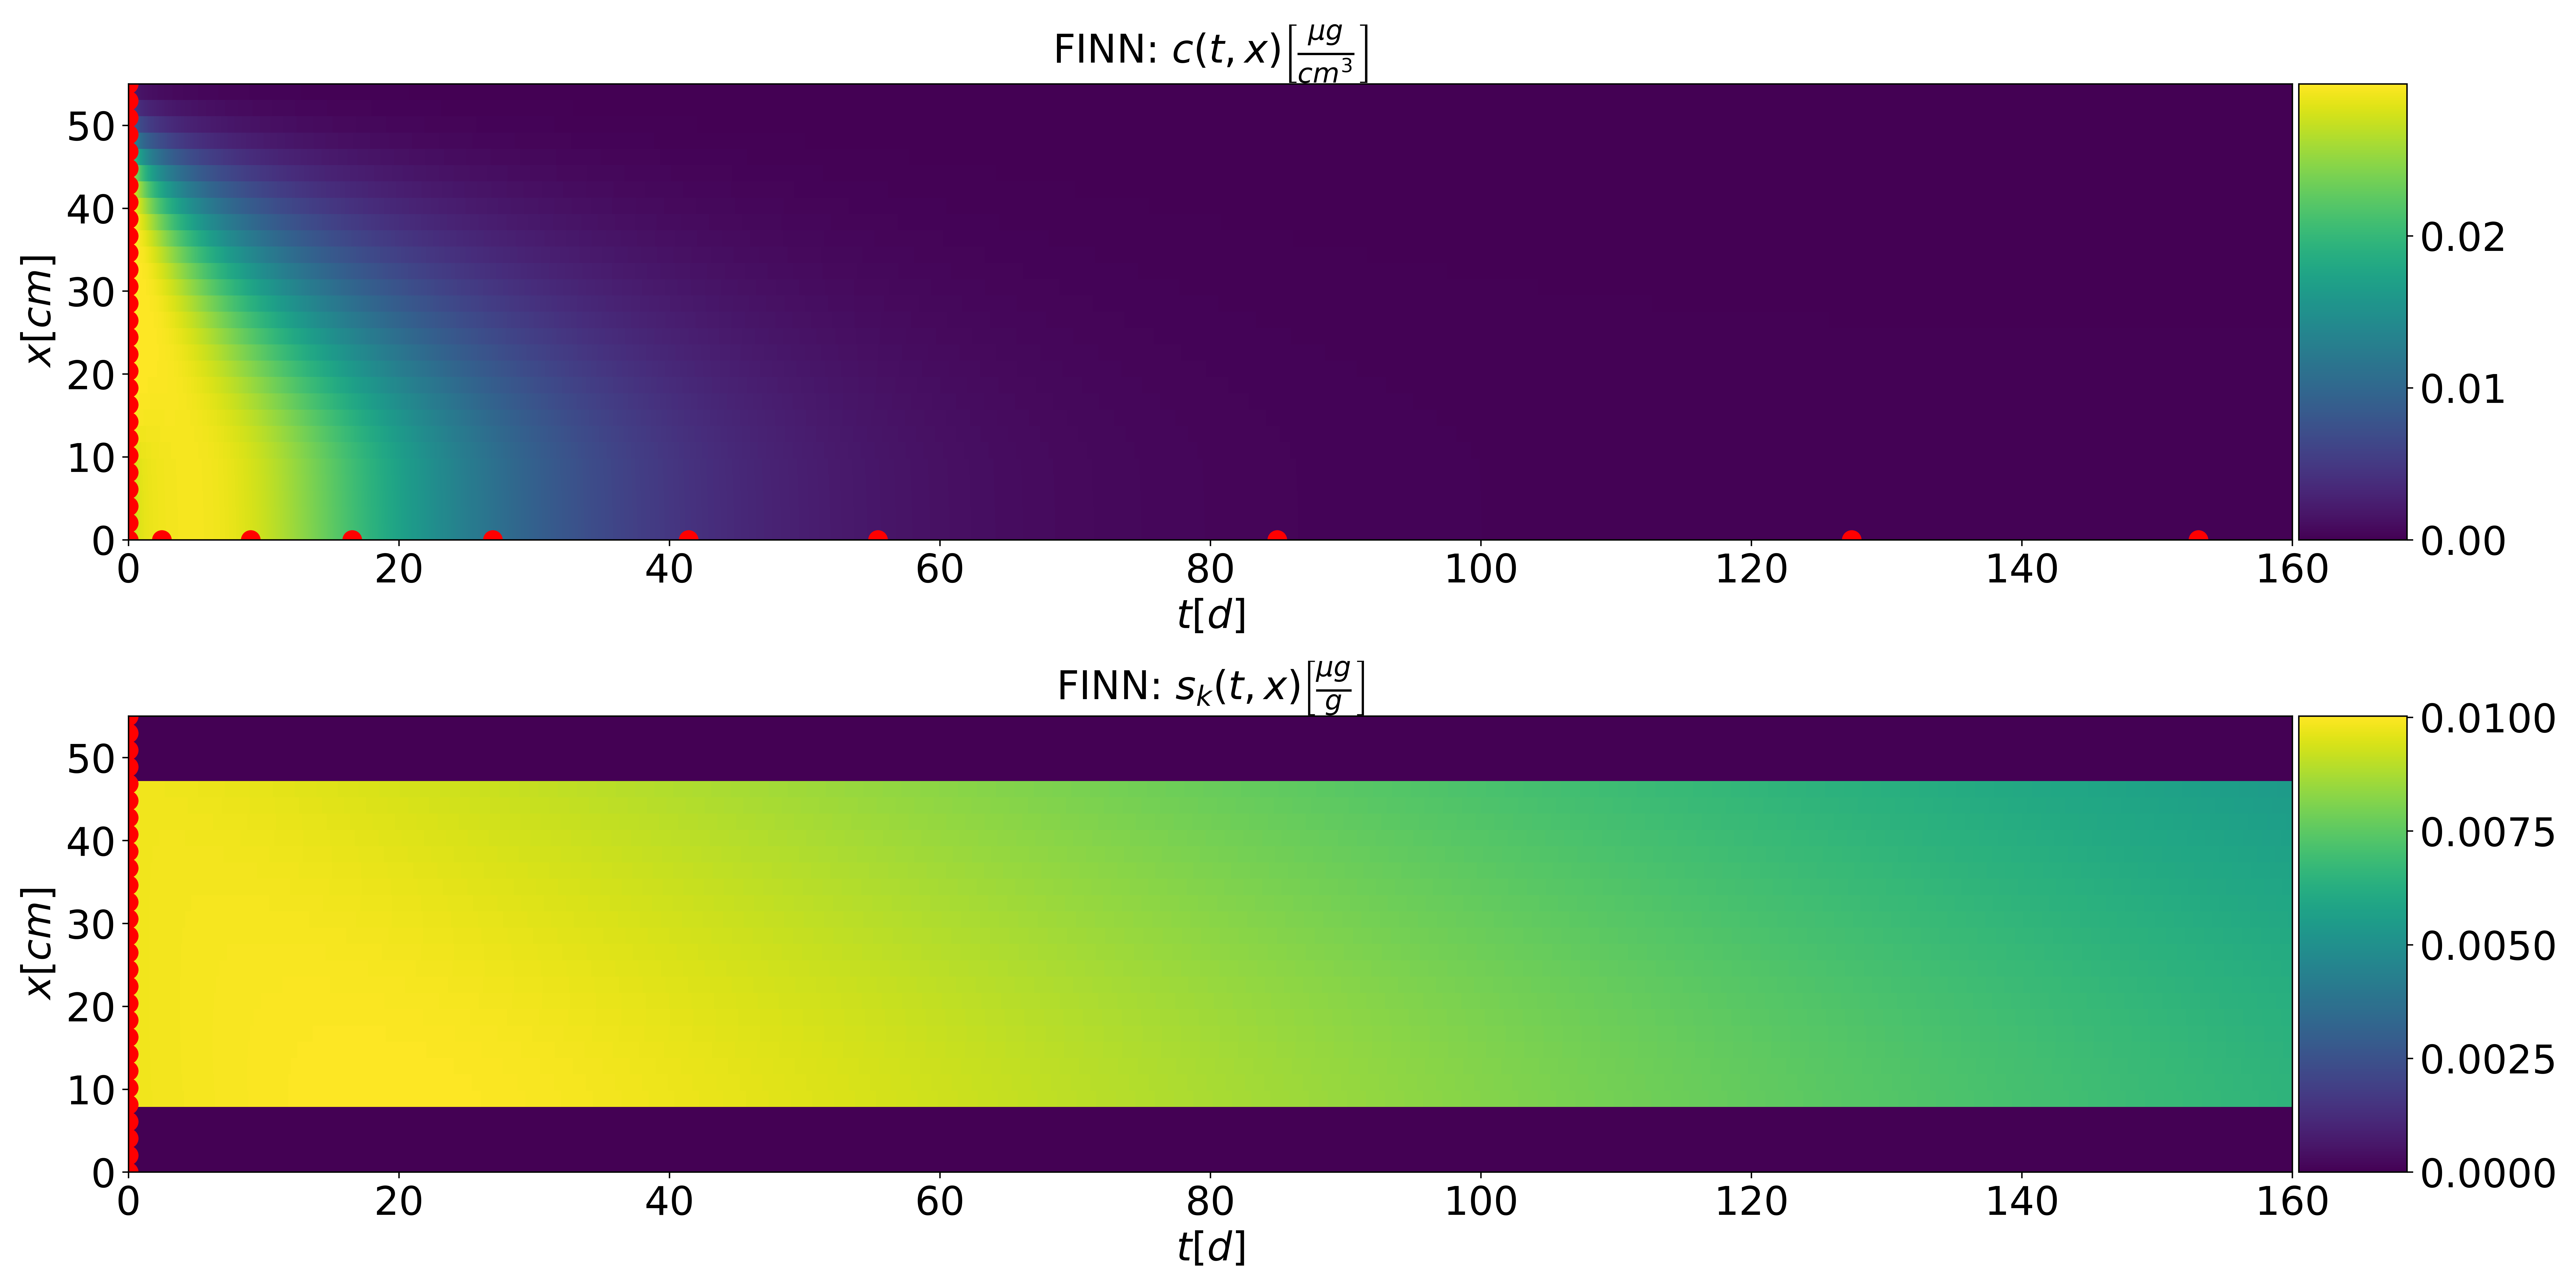
\includegraphics[width=\textwidth]{images/res_ov_exp_FGR_test_indp.png}
\caption[FINN predicted solution after testing, run h]{FINN prediction of $c$ (top) and $s_k$ (bottom) after testing time-independent functional relations. Red points describe initial conditions and BTC concentrations of experiment N1\_3 data, which were used for the loss calculation, run h.}
\label{fig:res_ov_exp_FGR_test_indp}
\end{figure}
\begin{figure}[h!]
	\centering
	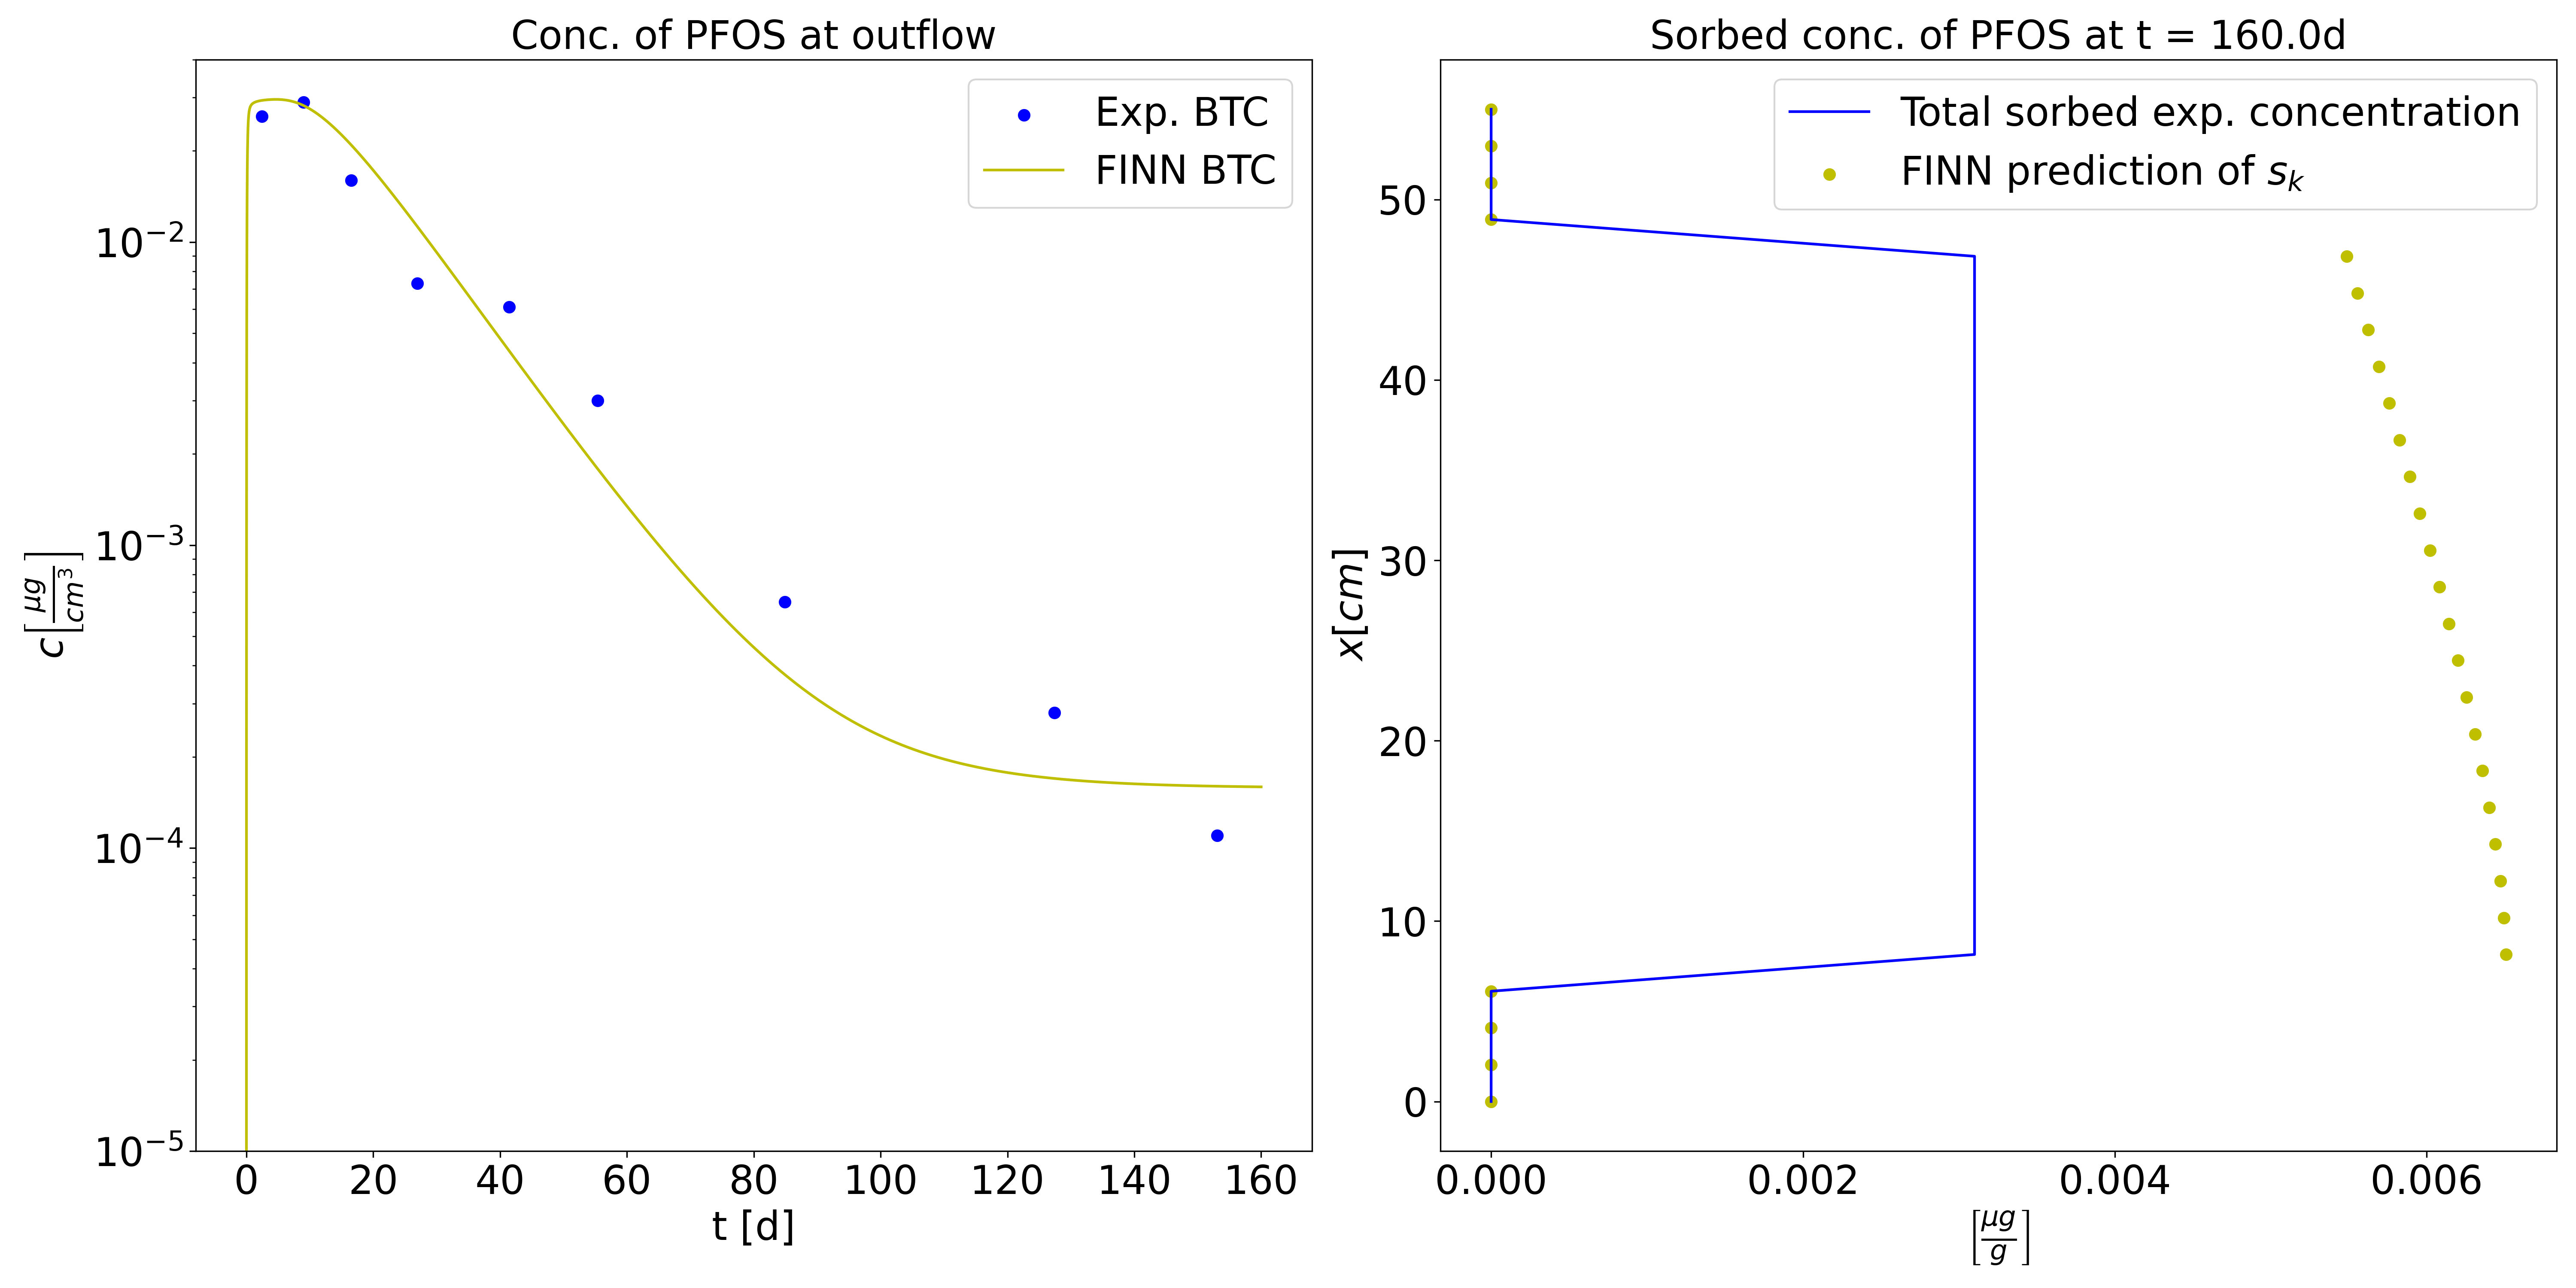
\includegraphics[width=\textwidth]{images/res_btc_exp_FGR_test_indp.png}
\caption[FINN predicted BTC after testing, run h]{BTC approximation after \textit{out-dis-test} (left). Comparison of \textit{out-dis-test} FINN predicted $s_k$ and experimental total sorbed concentration $s$ at the end of the experiment N1\_3 (right), run h.}
\label{fig:res_btc_exp_FGR_test_indp}
\end{figure}\\
The approximated BTCs are summarized in (Fig. \ref{fig:res_btc_exp_FGR_comp_indp}).
\begin{figure}[h]
	\centering
	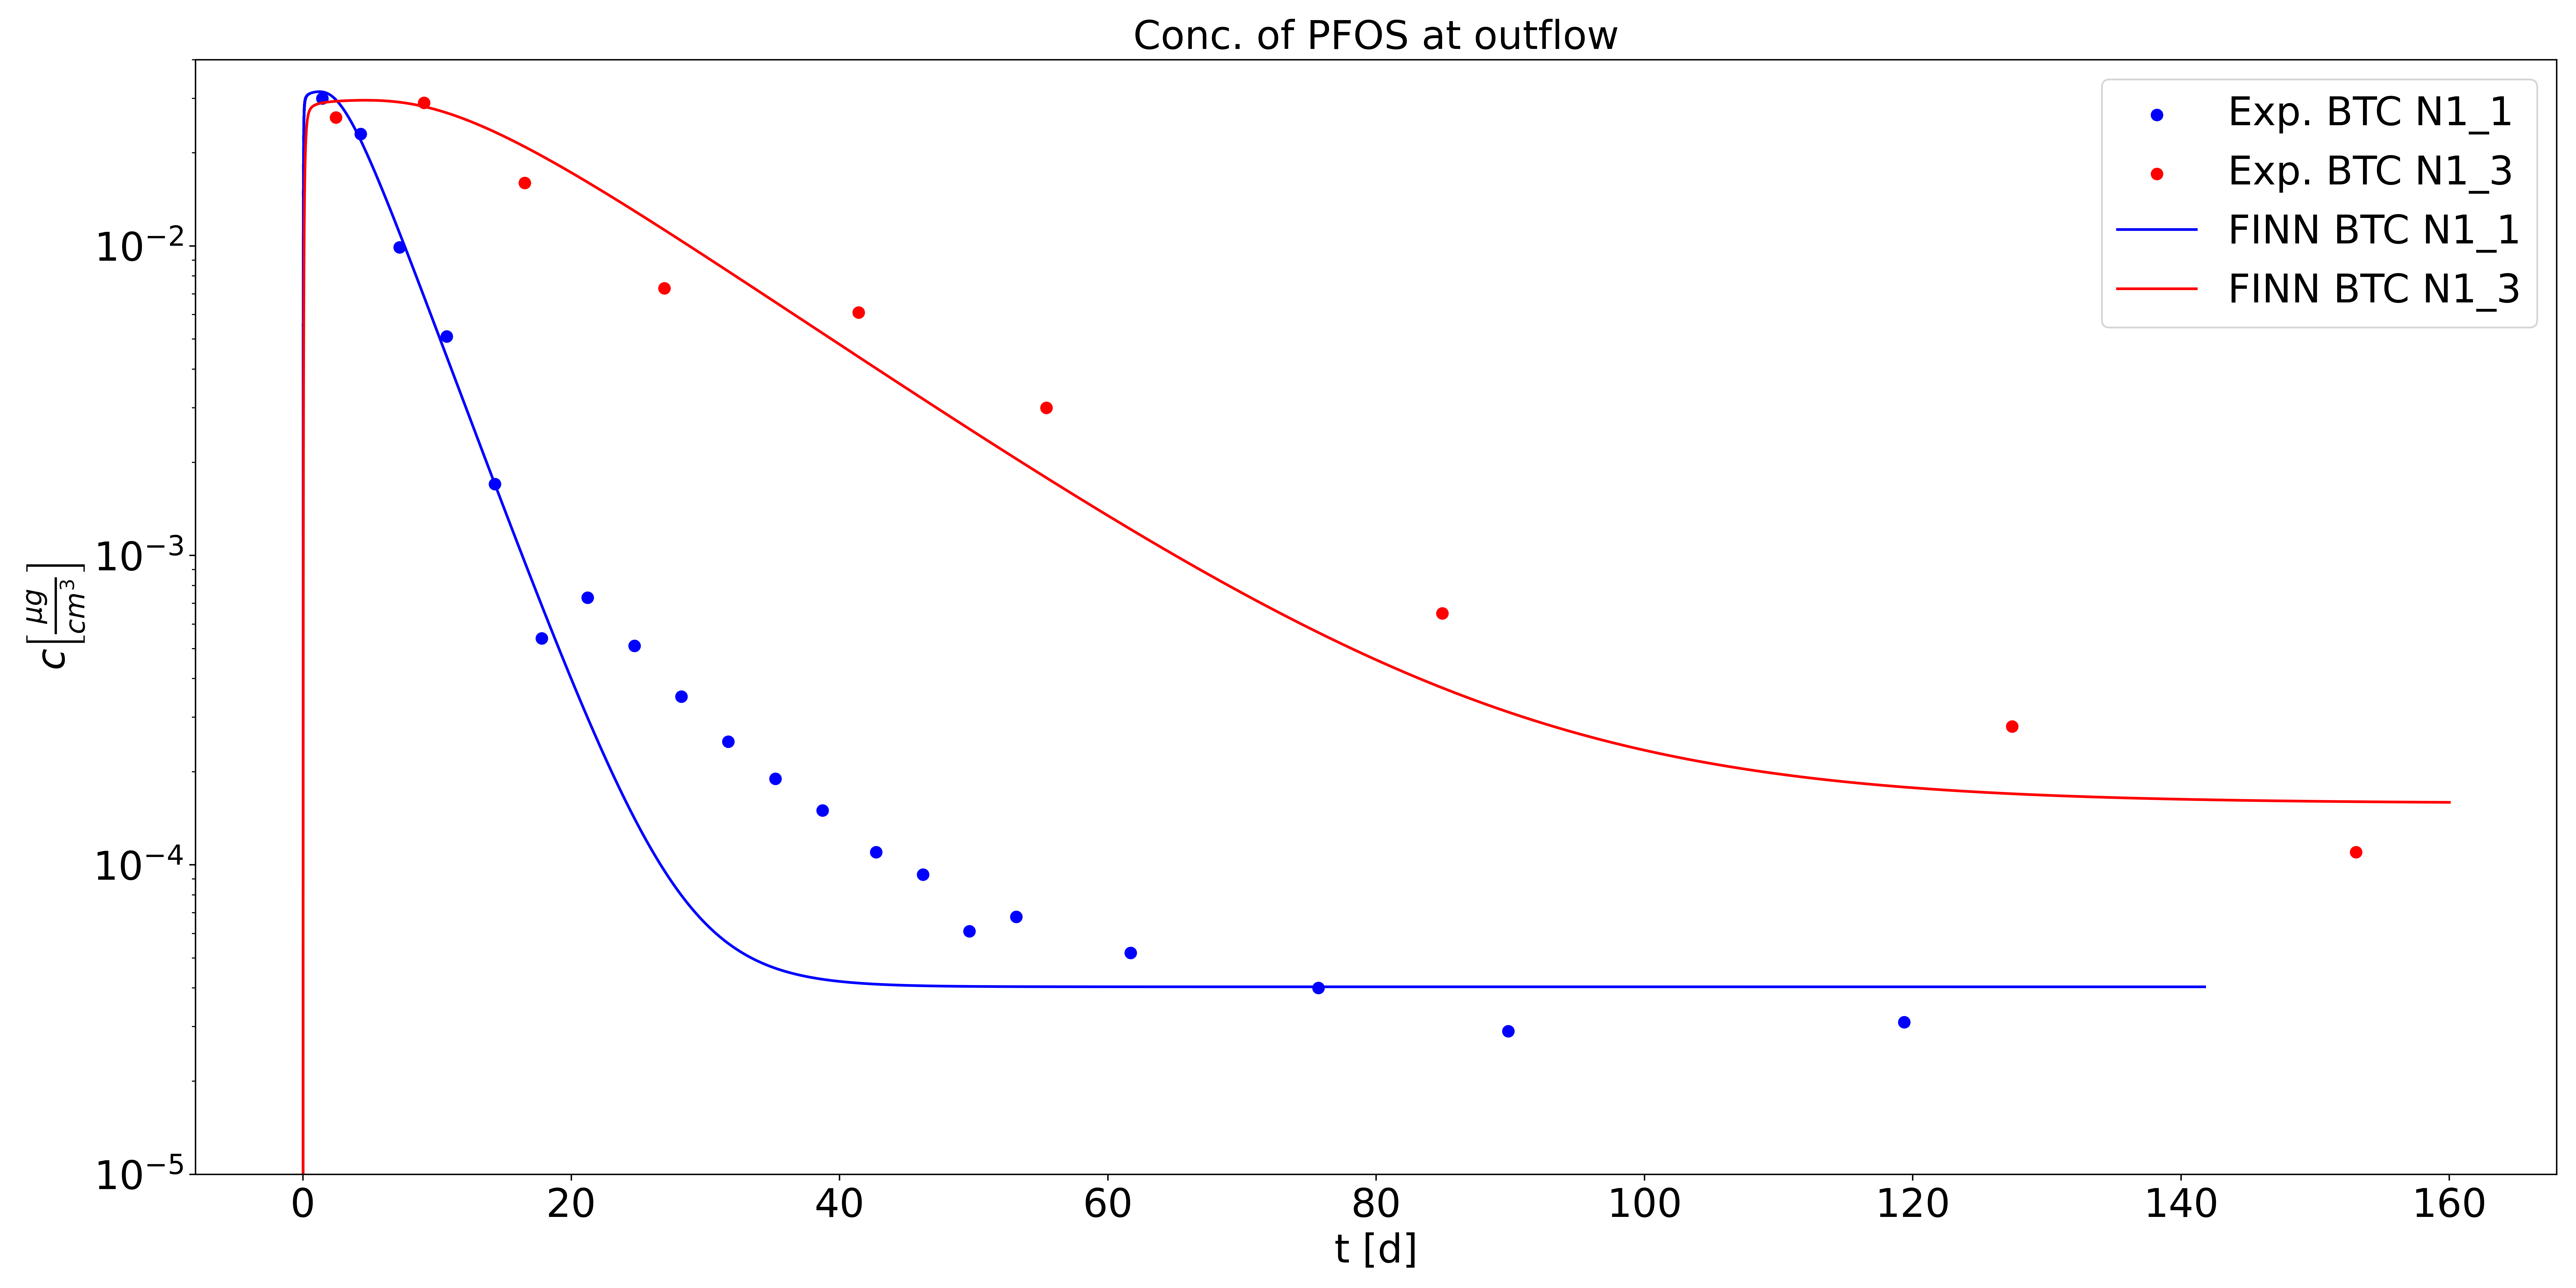
\includegraphics[width=\textwidth]{images/res_btc_exp_FGR_comp_indp.png}
\caption[Comparison of FINN predicted BTCs, run h]{Comparison of FINN predicted BTCs: Model trained with experiment N1\_1 (blue) and tested with experiment N1\_3 (red), run h.}
\label{fig:res_btc_exp_FGR_comp_indp}
\end{figure}
